%-----------------------------------------------------------------------------
% DOCUMENT CLASS
%-----------------------------------------------------------------------------
%\documentclass[12pt,a4paper,twoside,pdftex]{book}

% Put a comment on next line to output single-sided version
\def\twopage{1}

\ifx\twopage\undefined
  % Single-sided document
  \documentclass[12pt,a4paper,oneside,pdftex]{book}
\else
  % Double-sided document
 \documentclass[12pt,a4paper,twoside,pdftex]{book}
\fi

\pdfcompresslevel=9
%-----------------------------------------------------------------------------
% PACKAGES
%-----------------------------------------------------------------------------

\usepackage[italian, english]{babel}    % Last language is default one
\usepackage{graphicx} 
\usepackage[utf8]{inputenc}
\usepackage{sidecap}
\usepackage{url} 
\usepackage{amssymb} 
\usepackage{eurosym} 
\usepackage{subfig}
\usepackage{enumerate}
\usepackage{xtab}
\usepackage{fancyvrb}
\usepackage{sverb}
\usepackage{comment}
\usepackage{booktabs}
\usepackage{amsmath}
\usepackage{graphicx}
\usepackage{multirow}
\usepackage{longtable}
\usepackage{color}
\usepackage{microtype}
\usepackage{algorithm}
\usepackage[noend]{algpseudocode}
\usepackage[square, numbers, comma, sort&compress]{natbib} % Use the natbib reference package - read up on this to edit the reference style; if you want text (e.g. Smith et al., 2012) for the in-text references (instead of numbers), remove 'numbers'
%code java 
\usepackage{hyperref}

\definecolor{dkgreen}{rgb}{0,0.6,0}
\definecolor{gray}{rgb}{0.5,0.5,0.5}
\definecolor{mauve}{rgb}{0.58,0,0.82}

\usepackage{listings}

\lstset{frame=tb,
	language=Java,
	aboveskip=3mm,
	belowskip=3mm,
	showstringspaces=false,
	columns=flexible,
	basicstyle={\small\ttfamily},
	numbers=none,
	numberstyle=\tiny\color{gray},
	keywordstyle=\color{blue},
	commentstyle=\color{dkgreen},
	stringstyle=\color{mauve},
	breaklines=true,
	breakatwhitespace=true,
	tabsize=3
}
%code java end
\hypersetup{
    colorlinks,
    citecolor=black,
    filecolor=black,
    linkcolor=black,
    urlcolor=black
}

% Enhance verbatim style
\RecustomVerbatimEnvironment
  {verbatim} {Verbatim}
  {gobble=2, frame=lines}
\CustomVerbatimEnvironment
  {verbatim2} {Verbatim}
  {gobble=2}


%-----------------------------------------------------------------------------
% HEADERS AND FOOTERS
%-----------------------------------------------------------------------------


\usepackage{fancyhdr}
\pagestyle{fancy}

\renewcommand{\chaptermark}[1]{\markboth{#1}{}}
\renewcommand{\sectionmark}[1]{\markright{\thesection\ #1}}
% Remove footer text
\fancyhf{}

% Setup header and footer
\ifx\twopage\undefined
  % Single-sided document
  \fancyhead[R]{\bfseries\thepage}
  \fancyhead[L]{\bfseries\leftmark}
\else
  % Double-sided document
  \fancyhead[LE,RO]{\bfseries\thepage}
  \fancyhead[RE]{\bfseries\leftmark}
  \fancyhead[LO]{\bfseries\rightmark}
\fi

% Setup header and footer rules
\renewcommand{\headrulewidth}{0.5pt}
\renewcommand{\footrulewidth}{0pt}
\addtolength{\headheight}{0.5pt}
\fancypagestyle{plain}{
  \fancyhead{}
  \renewcommand{\headrulewidth}{0pt}
}
\setlength{\headheight}{14.5pt}


%-----------------------------------------------------------------------------
% PAGE MARGINS
%-----------------------------------------------------------------------------

\ifx\twopage\undefined
  % Single-sided document
  \addtolength{\oddsidemargin}{0cm} 
  \addtolength{\textwidth}{1.5cm}
  \addtolength{\headwidth}{1.5cm}
  \addtolength{\textheight}{1cm}
\else
  % Double-sided document
  \addtolength{\evensidemargin}{-2.0cm}
  \addtolength{\oddsidemargin}{.5cm}
  \addtolength{\textwidth}{1.5cm}
  \addtolength{\headwidth}{1.5cm}
  \addtolength{\textheight}{1cm}
\fi


%-----------------------------------------------------------------------------
% LEADING
%-----------------------------------------------------------------------------

\usepackage{setspace}
\onehalfspacing

%-----------------------------------------------------------------------------
% EQUATIONS
%-----------------------------------------------------------------------------



%-----------------------------------------------------------------------------
% DOCUMENT
%-----------------------------------------------------------------------------

\begin{document}
\newcommand{\rood}[1]{\textcolor{red}{[#1]}} 
\newcommand{\pending}[1]{\textcolor{cyan}{[#1]}}
%\newcommand{\ok}[1]{\textcolor{green}{[#1]}} 

% Choose Phys. Rev. style for bibliography
\bibliographystyle{unsrt}
% \nocite{*}   % to show non cited biblio

%------------------------------------------------ Cover page
\frontmatter
\thispagestyle{empty}

\begin{center}

	\textsc{Politecnico di Milano}\\
 	Scuola di Ingegneria dell'Informazione\\  

 	\par\vskip 0.2cm

 	
\includegraphics[width=7cm]{figures/polimi_logo.png}\\
  
 	\par\vskip 0.2cm  
  
  	\textsc{Polo territoriale di Como}\\
  	Master of Science in Computer Engineering\\  


  	\par\vskip 2cm
  	
\LARGE{ \bf	ECG-ira: An efficient mobile app for ECG analysis}


		
\end{center}

\par\vskip 1.5cm

\begin{flushleft}
  	\textbf{Supervisor}: Prof. Giuseppe Pozzi\\
  	\textbf{Co-Supervisors}: Ulisse Pizzagalli, Dr. Rodolfo Pizzuto \\
    \textbf{Assistant Supervisor}: 	\dots\dots\dots\dots\dots\dots \\
\end{flushleft}

\par\vskip 1cm

\begin{flushleft}
  	\textbf{Master Graduation Thesis by}: \\
  	Antonello Fodde - 817371 \\ 
  	Chai Botta - 817333 \\  
\end{flushleft}

\par\vskip 1cm

\begin{center}
 	Academic Year 2015-2016
\end{center}






% For double-sided document, leave a blank page
\ifx\twopage\undefined
\else
  \newpage \thispagestyle{empty} \null \newpage
\fi

%------------------------------------------------ Inscription

% Page without header
%\thispagestyle{empty} \null
%\vspace{4cm}
%\begin{flushright}
%\emph{Essentially, \\ all models are wrong, \\but some are useful.\\}
%\emph{\textit{\\(George E. P. Box)}}
%\end{flushright}

%------------------------------------------------ Abstract

% Page without header
\newpage \thispagestyle{empty} \newpage 
\chapter{Abstract}

Lorem ipsum dolor sit amet, consectetur adipiscing elit. Curabitur malesuada suscipit nisl, vitae gravida odio imperdiet a. Etiam sed auctor tellus. Donec sed mauris eget nibh luctus accumsan. Sed imperdiet purus in elit iaculis, non commodo nisl varius. Integer sit amet diam laoreet, viverra lacus id, placerat nisl. Aenean ultricies sollicitudin elit in sodales. Vivamus euismod eleifend justo, ac pellentesque risus. Donec eleifend, justo a pharetra laoreet, est dolor condimentum nulla, nec auctor ligula justo eget diam. Mauris augue eros, elementum quis vulputate eget, ullamcorper eget mauris.
Maecenas quis hendrerit velit. Donec vehicula dictum tellus, et aliquam sem viverra maximus. Maecenas gravida purus quis dui vulputate ornare. Morbi ac orci ut nunc tristique ultricies nec mattis massa. In imperdiet nisl ut risus faucibus, ut semper libero egestas. Nam imperdiet ullamcorper nunc, eu dictum felis dapibus a. Aliquam nec ante posuere, tristique dui semper, hendrerit erat. Nunc purus massa, lobortis a laoreet vel, posuere sit amet nisl. Duis ut viverra nisl. Pellentesque habitant morbi tristique senectus et netus et malesuada fames ac turpis egestas.

Nulla elit risus, efficitur condimentum erat id, laoreet ullamcorper tellus. Nam non rutrum massa. Suspendisse vitae mauris vitae arcu elementum molestie et at diam. Proin efficitur vehicula ligula, id rhoncus dui pulvinar et. Nunc nec ultrices nunc, ut cursus libero. Donec mattis vehicula ex eget efficitur. Ut tellus arcu, vehicula nec ullamcorper ut, vulputate eu arcu. In cursus ut justo non sodales. Sed massa urna, eleifend eu nisi eget, tincidunt efficitur nibh. Donec at molestie arcu. Duis elementum lectus at tristique scelerisque. Donec sodales purus viverra urna interdum, sit amet convallis velit lacinia. Aliquam mollis tempus rhoncus. Quisque ultricies nisi quis metus rhoncus mattis.
In fermentum facilisis tristique. Fusce ultricies quam id suscipit venenatis. Vestibulum hendrerit nibh eget ligula tristique, a tincidunt metus viverra. Aliquam finibus dui velit, a accumsan lacus tempus sit amet. Fusce in justo lorem. Mauris a porttitor justo, eget tincidunt erat. Ut quis semper risus. Aliquam eu malesuada metus. Aliquam erat volutpat. Sed ac diam finibus, pellentesque enim ut, commodo mi. Nam ligula odio, semper eget diam id, tempus cursus risus. Donec viverra, elit quis molestie ultrices, odio risus ornare orci, at eleifend nisl risus elementum tellus. Cum sociis natoque penatibus et magnis dis parturient montes, nascetur ridiculus mus. Suspendisse eu aliquet est, scelerisque vulputate justo.

Suspendisse egestas posuere lacinia. Integer non mi maximus, rhoncus massa eu, aliquam risus. Nam nisl nisi, semper nec efficitur eu, tincidunt vel justo. Sed vestibulum tristique consequat. Phasellus sodales nunc quis pharetra mattis. Pellentesque eu fermentum sem, vel efficitur odio. Suspendisse consectetur turpis et nisi viverra commodo. Quisque ornare porta nisi, eget aliquam nisl interdum sed. Nulla elementum quam sit amet enim mollis, in rhoncus felis lacinia. Nam vel justo purus. Nulla pellentesque ex in eros rutrum tincidunt. Morbi consequat felis a libero dictum, vel malesuada est dignissim. Maecenas diam lacus, laoreet ut quam vel, pharetra aliquet nisi. Suspendisse auctor aliquam odio eu tincidunt. Aenean lacinia semper diam. Suspendisse potenti.

\chapter{Sommario}
Negli ultimi anni il mercato della healthcare ha mantenuto una forte tendenza di interesse e subito un rapido sviluppo. Questo sviluppo ha sfruttato tutte le potenzialità rese disponibili dalle ultime tecnologie mobile: sono numerose le aziende che si sono specializzate nella creazione di dispositivi proprietari che svolgessero una determinata funzione: si va da quelli che fornissero supporti per il mondo del fitness, come l’analisi della massa corporea o del battito cardiaco, a quelli focalizzati nel campo medicale, come i sensori di pressione sanguigna o di livello di glucosio. Molti di questi hanno come potenzialità l’alta caratteristica di interfacciamento con l’utente, attraverso l’uso di mobile app che si sincronizzino con questi dispositivi e che analizzino i dati al fine di presentarli all’utente nel modo più accessibile possibile.\\
Il nostro lavoro vuole inserirsi in questo ambito, più specificatamente in quello medicale. Il nostro progetto nasce dal lavoro di alcuni studenti che ci hanno preceduto, e si presenta come una sua evoluzione in chiave moderna. Questo ci ha permesso di avere, come punto di partenza, un dispositivo e un software PC (precedentemente sviluppati) con cui interfacciarci. In particolare, il primo è un dispositivo di acquisizione di segnale ECG (elettrocardiogramma), chiamato ZEcg. La sua particolarità è rappresentata dalle ridotte dimensioni e dal suo interfacciamento di connessione, che sfrutta la tecnologia bluetooth, e quindi senza fili. Il software invece, nasce precedentemente, alle origini come software PC di visualizzazione ed analisi di aritmie di tracciati ECG. Successivamente è stato riadattato, al fine di aggiungere come funzionalità l’acquisizione in tempo reale dal dispositivo ZEcg di tracciati ECG.\\
Sfruttando il dispositivo ZEcg e gli algoritmi di analisi del precedente software, il progetto ha come fine la creazione di una mobile app per smartphone e tablet, che diventi un vero e proprio supporto per un medico specializzato, e che quindi fornisca tutte le funzionalità necessarie per acquisire, visualizzare ed analizzare un tracciato ECG. Inoltre l’app dovrà essere progettata per una massima estensibilità e compatibilità con più dispositivi mobile. Le caratteristiche di adattamento e rapidità che l’applicazione dovrà avere come primi obbiettivi, ci hanno portato al nome “ECG-ira”, che sta per “ECG-instantaneous responsive analyzer”. \\
Nel corso dei capitoli si analizzeranno i problemi riscontrati e le scelte implementative che hanno portato alla realizzazione del prodotto finale.




%\newpage \thispagestyle{empty} \newpage 
%\chapter{Abstract}

Lorem ipsum dolor sit amet, consectetur adipiscing elit. Curabitur malesuada suscipit nisl, vitae gravida odio imperdiet a. Etiam sed auctor tellus. Donec sed mauris eget nibh luctus accumsan. Sed imperdiet purus in elit iaculis, non commodo nisl varius. Integer sit amet diam laoreet, viverra lacus id, placerat nisl. Aenean ultricies sollicitudin elit in sodales. Vivamus euismod eleifend justo, ac pellentesque risus. Donec eleifend, justo a pharetra laoreet, est dolor condimentum nulla, nec auctor ligula justo eget diam. Mauris augue eros, elementum quis vulputate eget, ullamcorper eget mauris.
Maecenas quis hendrerit velit. Donec vehicula dictum tellus, et aliquam sem viverra maximus. Maecenas gravida purus quis dui vulputate ornare. Morbi ac orci ut nunc tristique ultricies nec mattis massa. In imperdiet nisl ut risus faucibus, ut semper libero egestas. Nam imperdiet ullamcorper nunc, eu dictum felis dapibus a. Aliquam nec ante posuere, tristique dui semper, hendrerit erat. Nunc purus massa, lobortis a laoreet vel, posuere sit amet nisl. Duis ut viverra nisl. Pellentesque habitant morbi tristique senectus et netus et malesuada fames ac turpis egestas.

Nulla elit risus, efficitur condimentum erat id, laoreet ullamcorper tellus. Nam non rutrum massa. Suspendisse vitae mauris vitae arcu elementum molestie et at diam. Proin efficitur vehicula ligula, id rhoncus dui pulvinar et. Nunc nec ultrices nunc, ut cursus libero. Donec mattis vehicula ex eget efficitur. Ut tellus arcu, vehicula nec ullamcorper ut, vulputate eu arcu. In cursus ut justo non sodales. Sed massa urna, eleifend eu nisi eget, tincidunt efficitur nibh. Donec at molestie arcu. Duis elementum lectus at tristique scelerisque. Donec sodales purus viverra urna interdum, sit amet convallis velit lacinia. Aliquam mollis tempus rhoncus. Quisque ultricies nisi quis metus rhoncus mattis.
In fermentum facilisis tristique. Fusce ultricies quam id suscipit venenatis. Vestibulum hendrerit nibh eget ligula tristique, a tincidunt metus viverra. Aliquam finibus dui velit, a accumsan lacus tempus sit amet. Fusce in justo lorem. Mauris a porttitor justo, eget tincidunt erat. Ut quis semper risus. Aliquam eu malesuada metus. Aliquam erat volutpat. Sed ac diam finibus, pellentesque enim ut, commodo mi. Nam ligula odio, semper eget diam id, tempus cursus risus. Donec viverra, elit quis molestie ultrices, odio risus ornare orci, at eleifend nisl risus elementum tellus. Cum sociis natoque penatibus et magnis dis parturient montes, nascetur ridiculus mus. Suspendisse eu aliquet est, scelerisque vulputate justo.

Suspendisse egestas posuere lacinia. Integer non mi maximus, rhoncus massa eu, aliquam risus. Nam nisl nisi, semper nec efficitur eu, tincidunt vel justo. Sed vestibulum tristique consequat. Phasellus sodales nunc quis pharetra mattis. Pellentesque eu fermentum sem, vel efficitur odio. Suspendisse consectetur turpis et nisi viverra commodo. Quisque ornare porta nisi, eget aliquam nisl interdum sed. Nulla elementum quam sit amet enim mollis, in rhoncus felis lacinia. Nam vel justo purus. Nulla pellentesque ex in eros rutrum tincidunt. Morbi consequat felis a libero dictum, vel malesuada est dignissim. Maecenas diam lacus, laoreet ut quam vel, pharetra aliquet nisi. Suspendisse auctor aliquam odio eu tincidunt. Aenean lacinia semper diam. Suspendisse potenti.


%------------------------------------------------ Lists

% Pages without header
\newpage \thispagestyle{empty} \newpage 
\tableofcontents

\newpage \thispagestyle{empty} \newpage 
\listoffigures

%\newpage \thispagestyle{empty} \newpage 
%\listofalgorithms
%\listofmyequations

%\newpage \thispagestyle{empty} \newpage 
%\listoftables
\newpage \thispagestyle{empty} \newpage 

%------------------------------------------------ Main matters

\mainmatter

% Chapter 1

\chapter{Introduction}
\label{Chapter1} 

ECG-ira stands for ECG (electrocardiogram) instant rapid analyzer and it is an android application developed for the acquisition, visualization and analysis of the electrocardiogram signals. The application acquires and stores  the record from the zecg acquisition device  (using the zecg device format) property of the Politecnico of Milan but it can also open and visualize other ecg format from other  devices. Ecg-ira is part of a greater and long term project (zecg itself was part of a first step). ECG-ira aims to exploit the reliability and performance of a complex software for electrocardiogram signal acquisition,  visualization  and processing within a smartphone device through a mobile application. Apart of the analysis algorithm already implemented during a past thesis (by Diego Ulisse Pizzagalli), the application was designed and implemented from scratch. During the process we dealt with the devices limitation in term of performance power and limited memory. We overcome many issues, related also to small and different screen size and density of pixel, due to the great number of different devices currently on the market. We had to exploit the multithreading and efficient memory usage strategies in order to achieve responsiveness and fulfill the medical requirement for an ECG compliant application. The result is an application which is easy to use because it follows all the best design principles according to the official Google guidelines for responsive UI and UX. By taking advantage of the multithreading capabilities and the usage of all the available cores into a device, we achieved an application which performs fast and well.\\
This thesis is structured as follows: 
\begin{itemize}
	\item After this introduction we give a brief but detailed overview about the heart, its functionalities and how an electrocardiogram is related to it by explaining starting from what it is an ecg to how heart electrical signals are detected and read.
	\item In the State of Art chapter we show the panorama of the actual devices for an ecg acquisition and some available applications on the market which allow to open and read an ecg record.
	\item Then it follows the Objective chapter in which we describe and explain the goal of this thesis work.
	\item The Requirements chapter is where we list functional and nonfunctional sets of features which came up during the planning phase. The final result should be compliant with all of them.
	\item The Problem chapter deals with all the issues related to the project development. Here we discussed about the problem of choosing a development platform with respect to another, the hardware limitation on a smartphone device and the problems strictly related to the ecg signals.
	\item The Solution choices chapter is where we explain and provide our reasonings to the implementation choices, from the platform choice to the programming language choice to why we decided to avoid using drawings libraries preferring a custom and proprietary implementation.
	\item In the System architecture chapter we provide a general overview of the project structure for both the acquisition device implementation and architecture both the mobile application structure and main functionalities.
	\item In the Implementation details chapter we described all the main components and Java classes. Here we provide also hints for future implementations and adaptations.
	\item In the Final result chapter we propose some screenshots, with descriptive captions and descriptions of the main screens of the application; then we go through a performance analysis of application by observing how it affects the memory, the cpu and the response time of some portion of the code. The tests were conducted on many different devices but only data from the older devices (2011) and the newest (November 2015) are compared.
	\item In the Conclusion chapter we sum up the overall results giving an overview of what has been done and providing some post considerations about the work done.
	\item In the Future works chapter we provide hints for further implementations in order to make ECG-ira really an all in one solution as an ECG mobile application. We also put our consideration on the future of the mobile software with respect to the desktop one, according to the new trends and the fact that the mobile environments is penetrating even more in our daily lives and can really positively change the way patients are connected with the health care providers.
\end{itemize}
% Chapter 2

\chapter{Electrocardiography overview}
\label{Chapter2} 

This chapter will introduce some basic but fundamental concepts about electrocardiography starting from the heart to the ECG and all issues related to the topic. We will start introducing the heart, its functionality and the entire circulatory system.\\
After that we will describe in details the electrical activity inside the heart and how heart beats are generated. Following there will be a description of the electrocardiogram and the ECG signals. In the last section of this chapter we will discuss about all the noises and interference related to the ECG signal during its acquisition. 

\section{The heart}
This chapter’s focus is to describe in details the human heart. We will start from the structure to end up describing the heart functionality.

\subsection{Human heart structure}
The human heart is an organ that pumps blood throughout the body via the circulatory system, supplying oxygen and nutrients to the tissues and removing carbon dioxide and other wastes.\\
This fundamental organ has four chambers: two upper chambers(the atrial) and two lower ones(the ventricles). The right atrium and the right ventricle together make up the “right heart”, and the left atrium and left ventricle make up the”left heart”. The two sides of the heart are separated by a muscle called the septum. \\
A double-walled sac called the pericardium, encases the heart, which serves to protect the heart and anchors it inside the chest. Between the outer layer, the parietal pericardium, and the inner layer, the serous pericardium, runs pericardial fluid, which lubricates the heart during contractions and movements of the lungs and diaphragm.
The heart outer wall consists of three layers. The outermost wall layer, or epicardium, is the inner wall of the pericardium.  The middle layer, or myocardium, contains the muscle that contracts. The inner layer, or endocardium, is the lining that contacts the blood.\\
The tricuspid valve and the mitral valve make up the atrioventricular (AV) valves, which connect the atria and the ventricles. The pulmonary semilunar valve separates the right ventricle from the pulmonary artery, and the aortic valve separates the left ventricle from the aorta. The heartstrings, or chordae tendineae, anchor the valves to heart muscles.\\
The sinoatrial node produces the electrical pulses that drive heart contractions.\\
\begin{figure}[ht!]
\centering
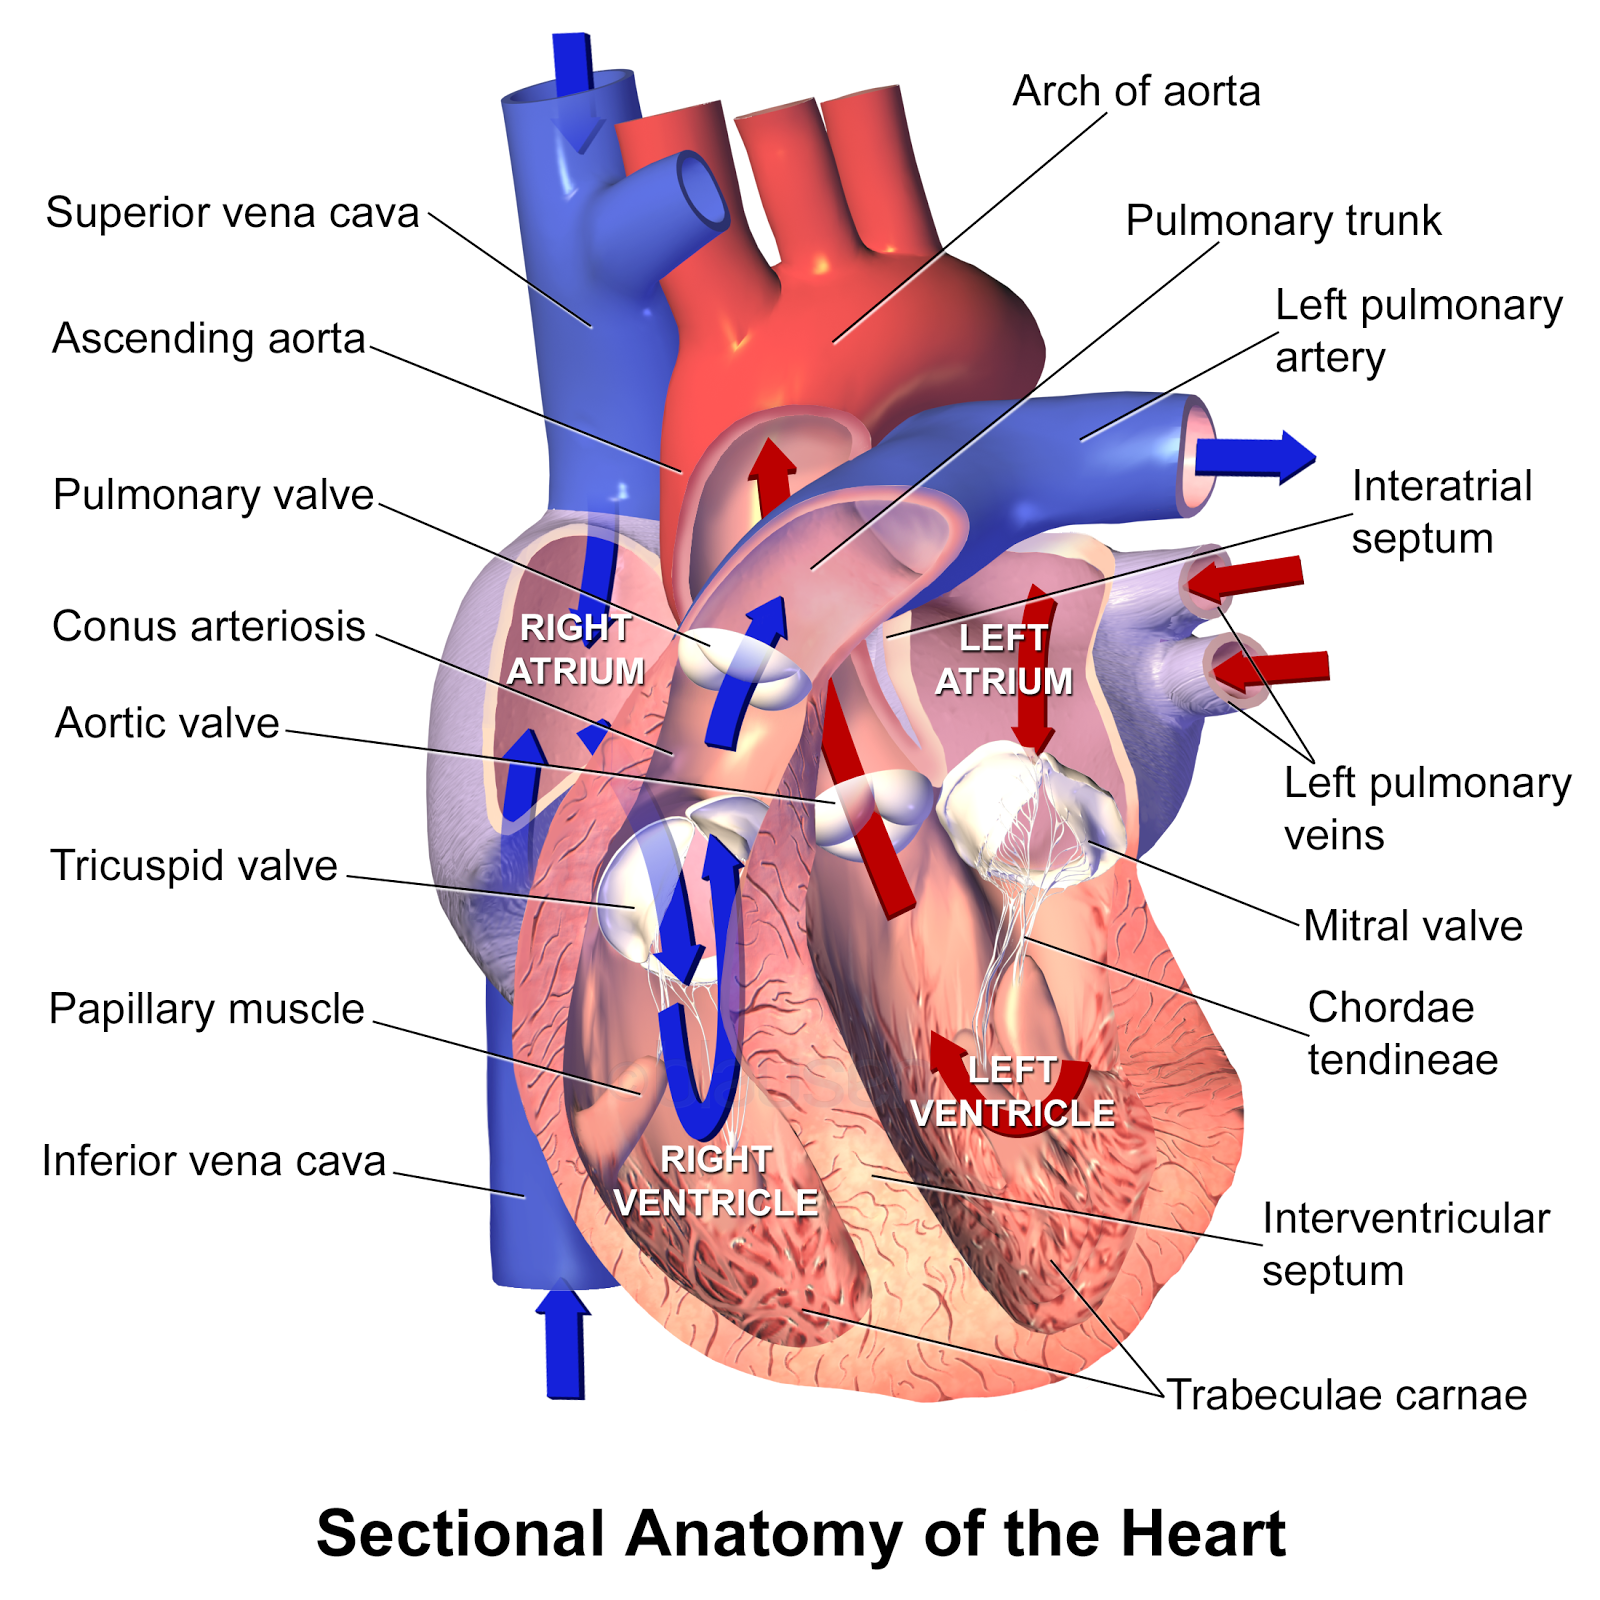
\includegraphics[width=100mm]{figures/ch2/1.png}
\caption{The human heart structure.\cite{ref1}}
\label{fig2.1}
\end{figure}

\subsection{Human heart function}
The heart circulates blood through two pathways: the pulmonary circuit and the systemic circuit.\\
In the pulmonary circuit, deoxygenated blood leaves the right ventricle of the heart via the pulmonary artery and travels to the lungs, then returns as oxygenated blood to the left atrium of the heart via the pulmonary vein.\\
In the systemic circuit, oxygenated blood leaves the body via the left ventricle to the aorta, and from there enters the arteries and capillaries where it supplies the body's tissues with oxygen. Deoxygenated blood returns via veins to the venae cavae, re-entering the heart's right atrium.\\
Of course, the heart is also a muscle, so it needs a fresh supply of oxygen and nutrients too. After the blood leaves the heart through the aortic valve, two sets of arteries bring oxygenated blood to feed the heart muscle. The left main coronary artery, on one side of the aorta, branches into the left anterior descending artery and the left circumflex artery. The right coronary artery branches out on the right side of the aorta.\\
Blockage of any of these arteries can cause a heart attack, or damage to the muscle of the heart. A heart attack is distinct from cardiac arrest, which is a sudden loss of heart function that usually occurs as a result of electrical disturbances of the heart rhythm. A heart attack can lead to cardiac arrest, but the latter can also be caused by other problems.\\
The heart contains electrical "pacemaker" cells, which cause it to contract — producing a heartbeat.\\
Each cell has the ability to be the 'band leader' and have everyone follow. In people with an irregular heartbeat, or atrial fibrillation, every cell tries to be the band leader, which causes them to beat out of sync with one another.\\
A healthy heart contraction happens in five stages:
\begin{enumerate}
	\item In the first stage (early diastole), the heart is relaxed.
	\item Then the atrium contracts (atrial systole) to push blood into the ventricle.
	\item Next, the ventricles start contracting without changing volume.
	\item Then the ventricles continue contracting while empty.
	\item Finally, the ventricles stop contracting and relax.
\end{enumerate}
Then the cycle repeats.\\
Valves prevent backflow, keeping the blood flowing in one direction through the heart.\\
\\
Some interesting data about the human heart are:
\begin{itemize}
	\item A human heart is roughly the size of a large fist.
	\item The heart weighs between about 280 to 340 grams in men and 230 to 280 grams in women.
	\item The heart beats about 100,000 times per day (about 3 billion beats in a lifetime).
	\item An adult heart beats about 60 to 80 times per minute.
	\item Newborns' hearts beat faster than adult hearts, about 70 to 190 beats per minute.
	\item The heart pumps about 6 quarts (5.7 liters) of blood throughout the body.
	\item The heart is located in the center of the chest, usually pointing slightly left
\end{itemize}
\begin{figure}[ht!]
	\centering
	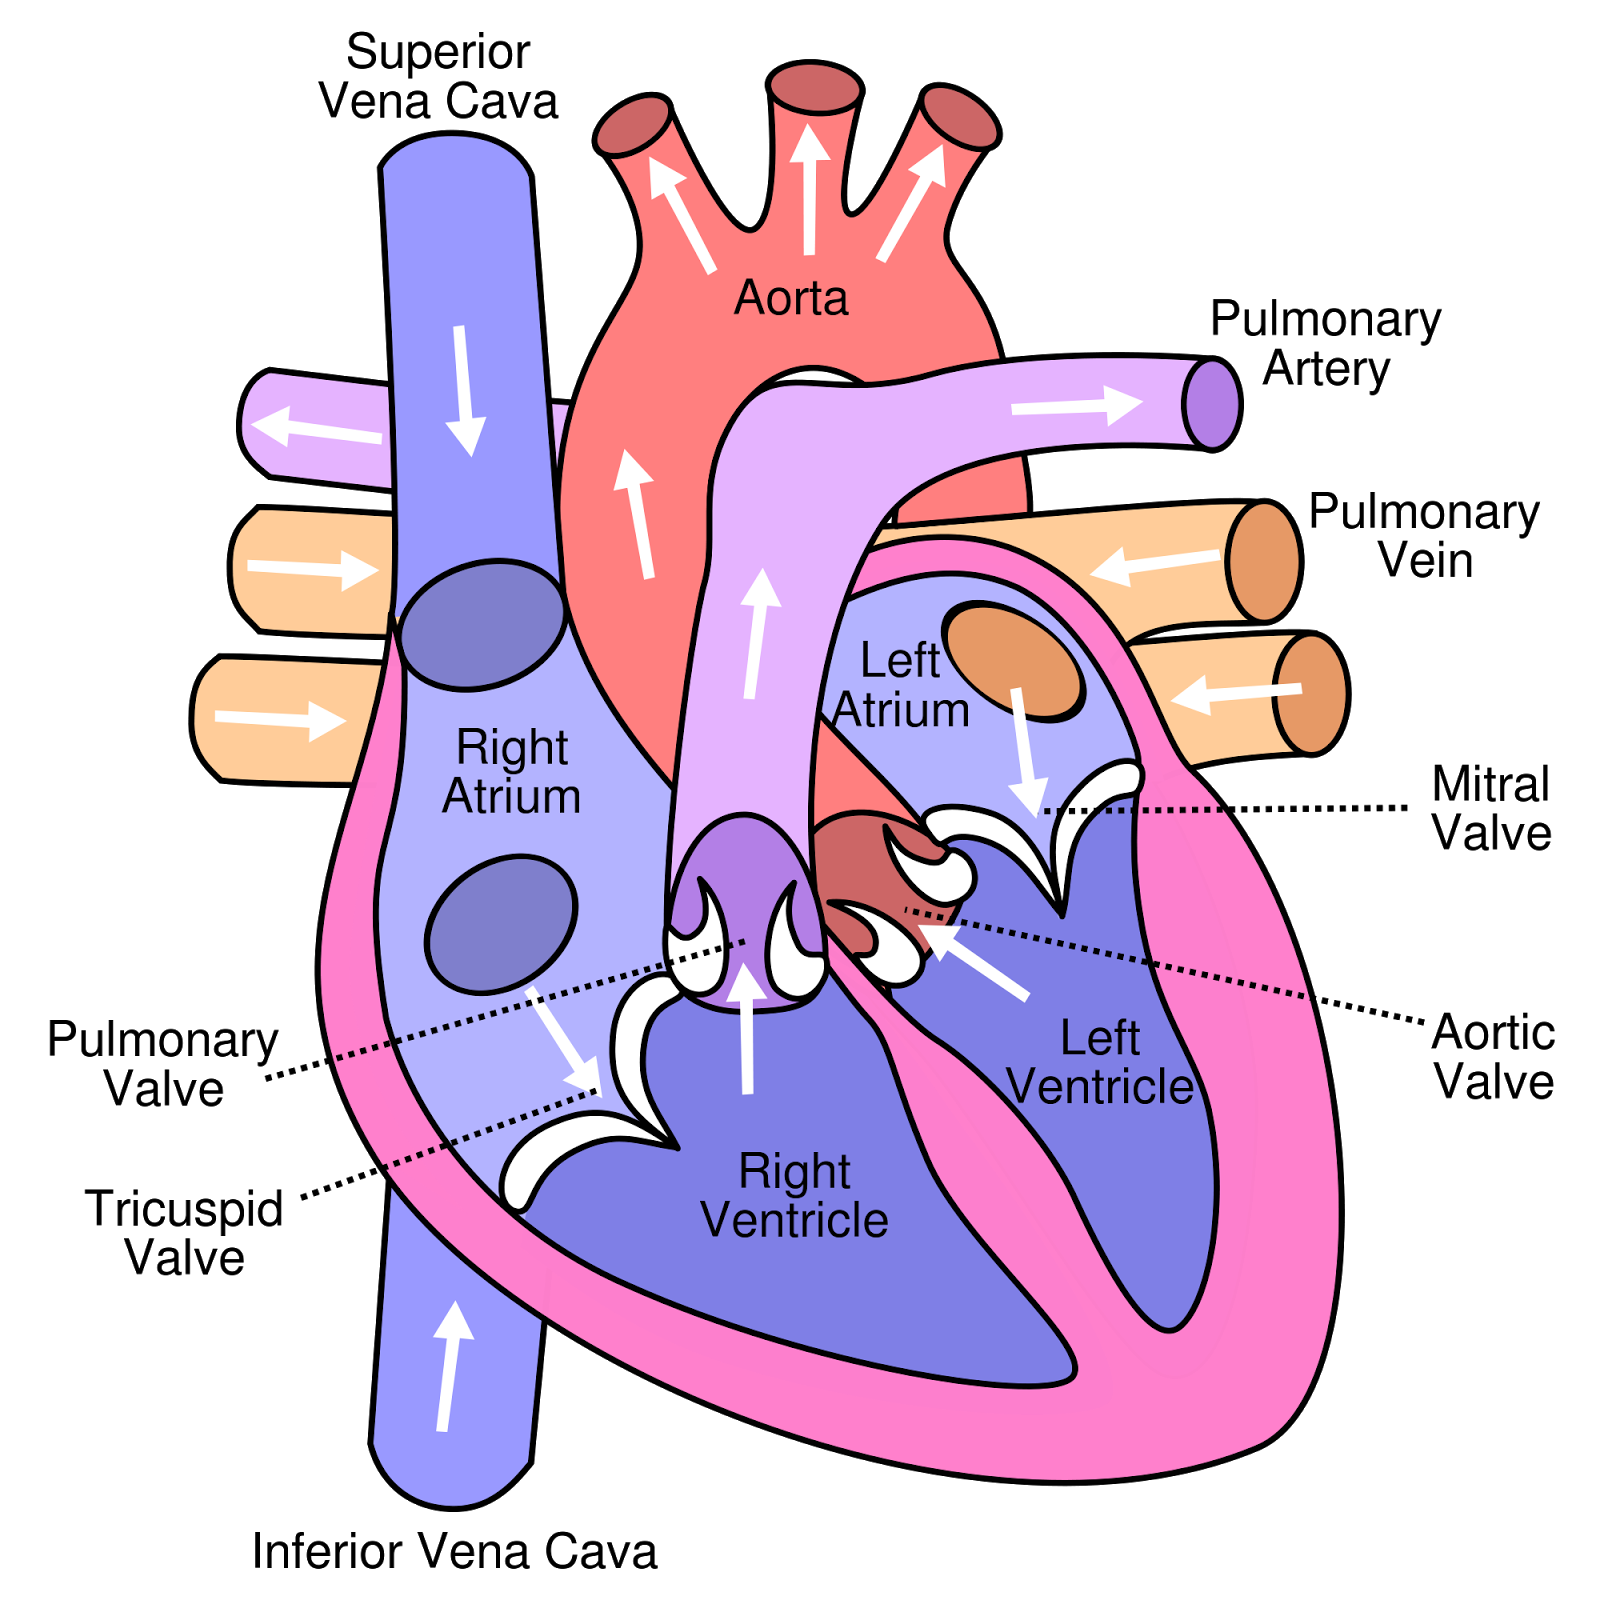
\includegraphics[width=90mm]{figures/ch2/2.png}
	\caption{The circulatory system with blood flow.}
	\label{fig2.2}
\end{figure}

\section{Heart electrical activity}
The heart has a natural pacemaker that regulates the pace or rate of the heart. It sits in the upper portion of the right atrium (RA) and is a collection of specializes electrical cells known as the SINUS or SINOATRIAL (SA) node.\\
Like the spark-plug of an automobile it generates a number of "sparks" per minute. Each "spark" travels across a specialized electrical pathway and stimulates the muscle wall of the four chambers of the heart to contract (and thus empty) in a certain sequence or pattern. The upper chambers or atria are first stimulated. This is followed by a slight delay to allow the two atria to empty. Finally, the two ventricles are electrically stimulated. In an car, the number of sparks per minute generated by a spark plug is increased when you press the gas pedal or accelerator. This revs up the motor. In case of the heart, adrenaline acts as a gas pedal and causes the sinus node to increase the number of sparks per minute, which in turn increases the heart rate. The release of adrenaline is controlled by the nervous system. The heart normally beats at around 72 times per minute and the sinus node speeds up during exertion, emotional stress, fever, etc., or whenever our body needs an extra boost of blood supply. In contrast, it slows down during rest or under the influence of certain medications. Well trained athletes also tend to have a slower heart beat.\\

\begin{figure}[ht!]
	\centering
	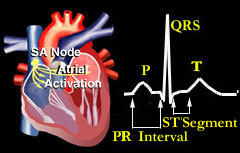
\includegraphics[width=60mm]{figures/ch2/3.png}
	\caption{The SA node fires and electrical impulses travels through the right and left atrium. \label{overflow}}
	\label{fig2.3}
\end{figure}
\begin{figure}[ht!]
	\centering
	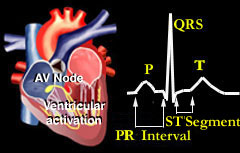
\includegraphics[width=60mm]{figures/ch2/4.png}
	\caption{The impulse then move to the ventricular area.}
	\label{fig2.4}
\end{figure}

The sequence of electrical activity within the heart is displayed in the diagrams above and occurs as follows:
\begin{enumerate}
	\item As the SA node fires, each electrical impulse travels through the right and left atrium. This electrical activity causes the two upper chambers of the heart to contract. This electrical activity and can be recorded from the surface of the body as a "P" wave" on the patient's EKG or ECG (electrocardiogram).
	\item The electrical impulse then moves to an area known as the AV (atrio-ventricular) node. This node sits just above the ventricles. Here, the electrical impulse is held up for a brief period. This delay allows the right and left atrium to continue emptying its blood contents into the two ventricles. This delay is recorded as a "PR interval." The AV node thus acts as a "relay station" delaying stimulation of the ventricles long enough to allow the two atria to finish emptying.
	\item Following the delay, the electrical impulse travels through both ventricles (via special electrical pathways known as the right and left bundle branches). The electrically stimulated ventricles contract and blood is pumped into the pulmonary artery and aorta. This electrical activity is recorded from the surface of the body as a "QRS complex". The ventricles then recover from this electrical stimulation and generates an "ST segment" and T wave on the ECG.
\end{enumerate}

\section{Electrocardiogram}
An electrocardiogram(abbreviated as ECG or EKG) is a test that measures the electrical activity of the heartbeat. With each beat, an electrical impulse (or wave) travels through the heart. This wave causes the muscle to squeeze and pump blood from the heart. A normal heartbeat on ECG will show the timing of the top and lower chambers.\\
The right and left atria or upper chambers make the first wave called a “P wave" following a flat line when the electrical impulse goes to the bottom chambers. The right and left bottom chambers or ventricles make the next wave called a “QRS complex." The final wave or “T wave” represents electrical recovery or return to a resting state for the ventricles.\\
\begin{figure}[ht!]
	\centering
	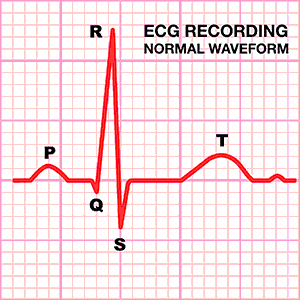
\includegraphics[width=60mm]{figures/ch2/5.png}
	\caption{An example of a normal ECG waveform. }
	\label{fig2.5}
\end{figure}
Each waves in the figure 2.5 is no other than the result of different views or perspectives of the waveforms generated from the current in the heart.\\
There are two type of ECGs recordings: the 12-lead ECG  and the rhythm strip. Both give valuable information about heart function.\\
We will focus our attention on the 12-lead ECG. It records information from 12 different views of the heart and provides a complete picture of electrical activity. The limb leads and the chest, or precordial, leads reflect information from the different planes of the heart. Different leads provide different information. The six limb leads I, II, III, augmented vector right (aVR), augmented vector left (aVL), and augmented vector foot (aVF) provide information about the heart’s frontal (vertical) plane. Leads I, II, and III require a negative and positive electrode for monitoring, which makes those leads bipolar. The augmented leads record information from one lead and are called unipolar.\\
The six precordials or V leads V1, V2, V3, V4, V5, and V6 provide information about the heart’s horizontal plane. Like the augmented leads, the precordial leads are also unipolar, requiring only a single electrode. The opposing pole of those leads is the center of the heart as calculated by the ECG.\\
The position of the leads are crucial for a right ECG recordings. It is common to use the so called Einthoven’s triangle, a set of positions to set up standard limb leads.
\begin{figure}[ht!]
	\centering
	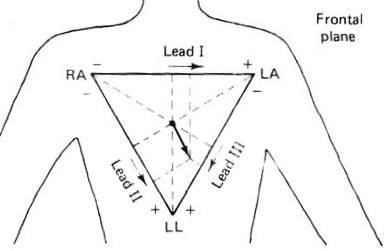
\includegraphics[width=80mm]{figures/ch2/6.png}
	\caption{The Einthoven’s triangle show the right position to place leads over the chest.}
	\label{fig2.6}
\end{figure}
The electrodes for leads I, II, III are about equidistant from the heart and form an equilateral triangle.

\subsection{Lead I}
It provides a view of the heart that shows current moving from right to left. Because the current flows from negative to positive, the positive electrode for this lead is placed on the left arm or on the left side of the chest; the negative electrode is placed on the right arm. Lead I produces a positive deflection on ECG tracings and is helpful in monitoring atrial and hemiblock.

\subsection{Lead II}
Lead II produces a positive deflection. Place the positive electrode on the patient’s left leg and the negative electrode on the right arm. For continuous monitoring, place the electrodes on the torso for convenience, with the positive electrode below the lowest palpable rib at the left midclavicular line and the negative electrode below the right clavicle. The current travels down and to the left in this lead. Lead II tends to produce a positive, high voltage deflection, resulting in tall P, R, and T waves. This lead is commonly used for routine monitoring and is useful for detecting sinus node and atrial arrhythmias.

\subsection{Lead III}
Lead III produces a positive deflection. The positive electrode is placed on the left leg; the negative electrode, on the left arm. Along with lead II, this lead is useful for detecting changes associated with an inferior wall myocardial infarction. The axes of the three bipolar limb leads I, II, and III form a triangle around the heart and provide a frontal plane view of the heart.

\subsection{Augmented leads}
Leads aVR, aVL, and aVF are called augmented leads. They measure electrical activity between one limb and a single electrode. Lead aVR provides no specific view of the heart. Lead aVL shows electrical activity coming from the heart’s lateral wall. Lead aVF shows electrical activity coming from the heart’s inferior wall.

\subsection{Precordials leads}
The six unipolar precordial leads (V1, V2, V3, V4, V5  and V6) are placed in sequence across the chest and provide a view of the heart’s horizontal plane.
\begin{itemize}
	\item Lead V1—The precordial lead V1 electrode is placed on the right side of the sternum at the fourth intercostal rib space. This lead corresponds to the modified chest lead MCL1 and shows the P wave, QRS complex, and ST segment particularly well. It helps to distinguish between right and left ventricular ectopic beats that result from myocardial irritation or other cardiac stimulation outside the normal conduction system. Lead V1 is also useful in monitoring ventricular arrhythmias, ST-segment changes, and bundle-branch blocks.
	\item Lead V2—Lead V2 is placed at the left of the sternum at the fourth intercostal rib space.
	\item  Lead V3—Lead V3 goes between V2 and V4. Leads V1, V2, and V3 are biphasic, with both positive and negative deflections. Leads V2 and V3 can be used to detect ST-segment elevation.
	\item Lead V4—Lead V4 is placed at the fifth intercostal space at the midclavicular line and produces a biphasic waveform.
	\item Lead V5—Lead V5 is placed at the fifth intercostal space at the anterior axillary line. It produces a positive deflection on the ECG and, along with V4, can show changes in the ST segment or T wave.
	\item Lead V6—Lead V6, the last of the precordial leads, is placed level with V4 at the midaxillary line. This lead produces a positive deflection on the ECG.
\end{itemize}
\begin{figure}[ht!]
	\centering
	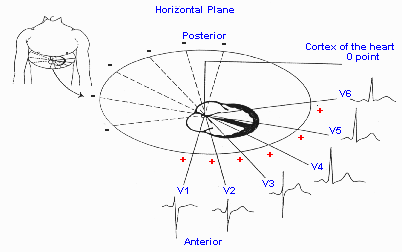
\includegraphics[width=90mm]{figures/ch2/7.png}
	\caption{Precordial leads and their position related to the heart and the chest horizontal plane.}
	\label{fig2.7}
\end{figure}

\subsection{How to read a ECG record}
Waveforms produced by the heart’s electrical current are recorded on graphed ECG paper by a stylus. An ECG paper consists of horizontal and vertical lines forming a grid. A piece of ECG paper is called an ECG strip or tracing.
\begin{figure}[ht!]
	\centering
	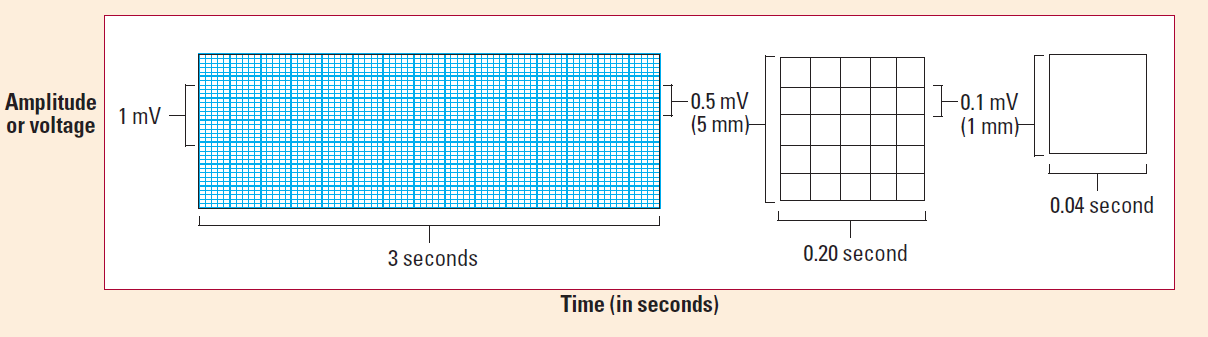
\includegraphics[width=130mm]{figures/ch2/8.png}
	\caption{A typical ECG paper.}
	\label{fig2.8}
\end{figure}
The horizontal axis of the ECG strip represents time. Each small block equals 0.04 second, and five small blocks form a large block, which equals 0.2 second. This time increment is determined by multiplying 0.04 second (for one small block) by 5, the number of small blocks that compose a large block. Five large blocks equal 1 second (5 x 0.2). When measuring or calculating a patient’s heart rate, a 6-second strip consisting of 30 large blocks is usually used. The ECG strip’s vertical axis measures amplitude in millimeters (mm) or electrical voltage in millivolts (mV). Each small block represents 1 mm or 0.1 mV; each large block, 5 mm or 0.5 mV. To determine the amplitude of a wave, segment, or interval, count the number of small blocks from the baseline to the highest or lowest point of the wave, segment, or interval.

\section{Noises and interferences}
Obtaining a reliable ECG recording is still an issue. In fact there may occur many problems interfering with the signals. Some of these problems include artifacts from patient movement and poorly placed or poorly functioning equipment.

\subsection{Artifact}
Artifact , also called waveform interference, may be seen with excessive movement (somatic tremor). The baseline of the ECG appears wavy, bumpy, or tremulous. Dry electrodes may also cause this problem to occur due to poor contact.
\begin{figure}[ht!]
	\centering
	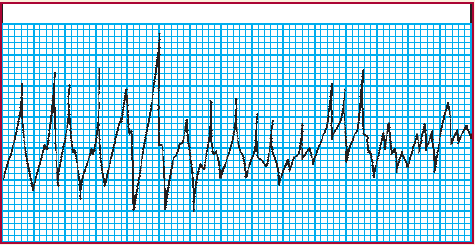
\includegraphics[width=90mm]{figures/ch2/9.png}
	\caption{ECG waveform interference due to artifact may cause monitoring to fail due to unreadable signals.}
	\label{fig2.9}
\end{figure}

\subsection{Interference}
Electrical interference, also called 60-cycle interference, is caused by electrical power leakage. It may occur due to interference from other room equipment or improperly grounded equipment. As a result, the lost current pulses at a rate of 60 cycles per second. This interference appears on the ECGs as a baseline that is thick and unreadable.
\begin{figure}[ht!]
	\centering
	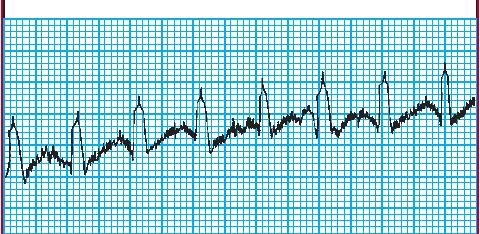
\includegraphics[width=90mm]{figures/ch2/10.png}
	\caption{Electrical interference causes the baseline to be unstable and the signal is corrupted.}
	\label{fig2.10}
\end{figure}

\subsection{Wandering baseline}
A wandering baseline undulates, meaning that all waveforms are present but the baseline is not stationary.  It can be caused by movement if the chest wall during respiration, poor electrode placement, or poor electrode contact.
\begin{figure}[ht!]
	\centering
	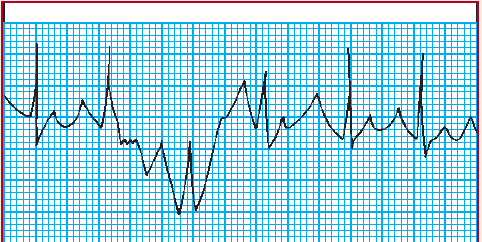
\includegraphics[width=90mm]{figures/ch2/11.png}
	\caption{An example of baseline wandering due to artifacts.}
	\label{fig2.11}
\end{figure}

\subsection{Faulty equipment}
Faulty equipment, such a s broken lead wires and cables, can also cause monitoring problems.
% Chapter 2

\chapter{State of Art}
\label{Chapter3} 

\section{Device}
The personal health care market has changed a lots and recently new products and devices are showing up on the market. We will describe briefly the most relevant and similar products as mobile ECG acquisition devices.  We evaluate the following solutions:
\begin{itemize}
	\item Mortara ELI 10 Mobile
	\item Philips DigiTrak XT Holter Recorder
	\item M-Trace (PC) Mobile
	\item ECG Expert 
\end{itemize}

\subsection{Mortara ELI 10 Mobile}
This device offers an all in one solution for 12 leads ECG acquisition. It is compact and complete as it provides an alphanumeric keyboard and a screen for real time visualization and the possibility to send the record via GPRS/3G channels. For each devices a SIM card is required . The device can also read and interpret the ECG supporting the doctor. Interesting feature is its great interoperability with the main ECG data management systems.
\begin{figure}[ht!]
	\centering
	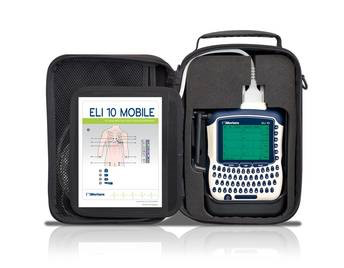
\includegraphics[width=90mm]{figures/ch3/1.png}
	\caption{Mortara ELI 10 Mobile, ECG acquisition device box.}
	\label{fig3.1}
\end{figure}

\subsection{Philips DigiTrak XT Holter Recorder}
This is the smaller acquisition device on the market. Thanks to a proprietary algorithm from Philips it can derive all the 12 ECG leads using only 5 leads. It weighs 62g and the internal battery lasts till 7 days. It also has a small screen showing 1 real time signal at a time.
\begin{figure}[ht!]
	\centering
	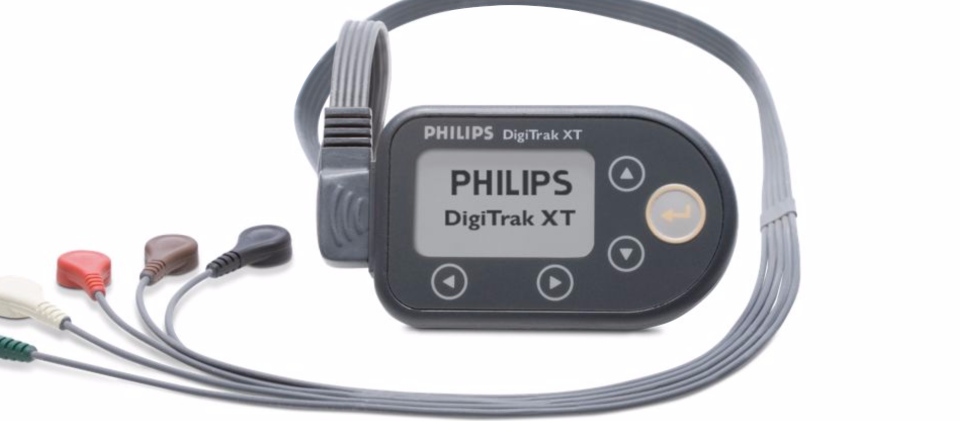
\includegraphics[width=90mm]{figures/ch3/2a.png}
	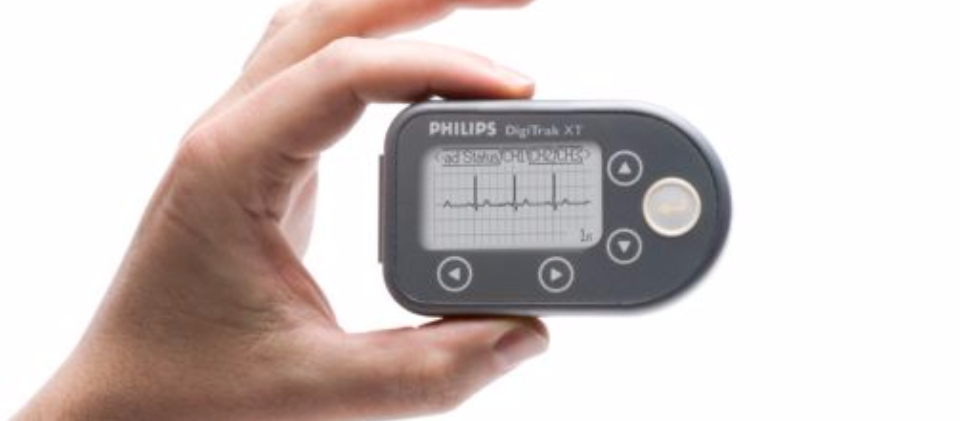
\includegraphics[width=90mm]{figures/ch3/2b.png}
	\caption{DigiTrack, the ECG visualization.}
	\label{fig3.2}
\end{figure}

\subsection{AliveCor ECG}
An innovative solution even though it doesn’t offer a complete solution for ECG acquisition and analysis. This small sensor can be attached on the back of your smartphone making it an ECG acquisition device. It can record only one ECG signal (D1), so also the analysis is limited to a few types of arrhythmias . The record length is also limited to 5 minutes.
\begin{figure}[ht!]
	\centering
	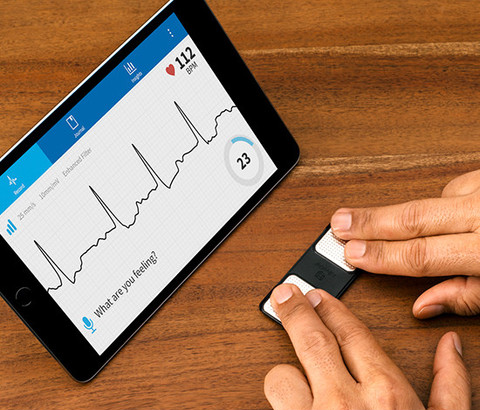
\includegraphics[width=90mm]{figures/ch3/3.png}
	\caption{AliveCor device real time acquisition on a tablet.}
	\label{fig3.3}
\end{figure}

\subsection{M-Trace (PC)Mobile}
M-Trace PC is an completed 12 leads ECG acquisition device. With the device it comes a mobile application and a desktop pc application used to visualize and analyze the ecg signals. The device is really portable with dimensions 95x64x28mm.  The company offers also a more portable device (M-Trace Mobile) to be used by privates at their home. The mobile version cannot acquire a full record but only test records with 6 leads. Its main purpose it to send the test records via GSM/GPRS to the doctor for a faster review.
\begin{figure}[ht!]
	\centering
	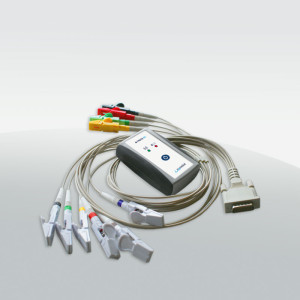
\includegraphics[width=60mm]{figures/ch3/4a.png}
	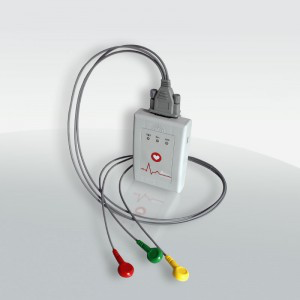
\includegraphics[width=60mm]{figures/ch3/4b.png}
	\caption{M-Trace PC device for ECG acquisition.}
	\label{fig3.4}
\end{figure}

\subsection{ECG Expert}
ECG Expert produced by CSE Medical is a completed solution for ECG acquisition. The device comes with fully supported software for both PC desktop (Windows and Mac) both smartphones  (Android, iOS). The device is rechargeable and makes use of a wireless connection via Bluetooth as exchanges data communication with the handheld smartphone or PC software.
\begin{figure}[ht!]
	\centering
	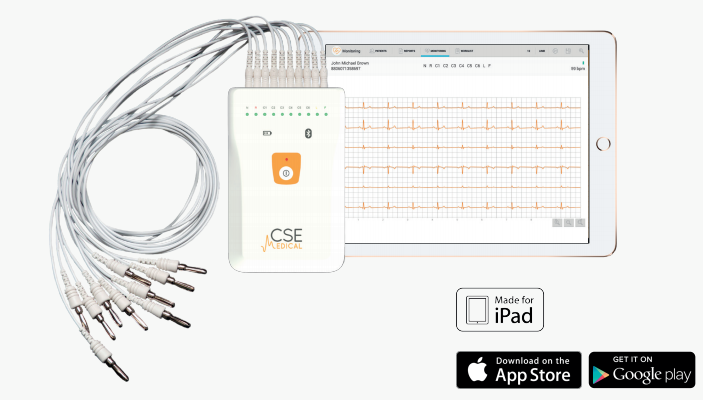
\includegraphics[width=60mm]{figures/ch3/5.png}
	\caption{M-Trace PC device for ECG acquisition.}
	\label{fig3.5}
\end{figure}

\section{Mobile application}
There are already mobile applications on the market store for ECG visualization and analysis supporting different formats. We can distinguish applications that only visualize the signal and the ones that also apply some analysis on the ECG signals. We listed only applications on the Google Play Store, so only Android applications because they are the only comparable with the solution we propose.

\subsection{Visualization only application}
The application on the market able to visualize the ECG signal are:
\begin{itemize}
	\item \textit{StribogECG}: an Android application based on an open source project under GLP v3 licence. It uses Biosig library to read ECG formats such as scp, xml (hl7), ecg and dgf. The software is only provided as it is and it requires to the user to already have the ecg files stored in those supported formats.
	\item \textit{AndroidECG}: application on beta release, it was developed by Paco Gonzàles as thesis project during the Master course in Computer Science at the University of Murcia. The application is able to show ECG signals of the following formats: binary, scp, 212. As additional feature it is a basic analysis over the signal to detect QRS complex, P waves, ST segments and T waves. It is also possible to send the ECG record via email.
\end{itemize}

\subsection{Visualization and Analysis}
The applications on the market that also provide a more detailed analysis over the ECG signal are all bind to a specific proprietary acquisition device. By this way they lack the compatibility and interoperability requirement with other software and ECG formats.
\begin{itemize}
	\item \textit{M-Trace PC}: the application was developed by \textit{M4Medical}, a Poland company providing medical devices for professionals and private customers. The application only works with the company 12-channel ECG M-Trace PC register device. The main features are the real-time monitoring interface, a patients’ database management system and the possibility to share the record.
	\item \textit{ECG Expert}: developed by \textit{CSE Medical} the application works only connected to an ECG-Expert acquisition device. The main features are the real-time view of the acquisition, the analysis of the record providing information about QRS complex and heart rate, the possibility to manage patient information bind to the record and a heartbeat Normal/Abnormal classifier.
\end{itemize}
One last mobile application, which is not strictly related to ECG signal visualization and analysis but it worth to be mentioned, is the \textit{ECG Interpretation}. This application instead provides  enough detailed information about how to read and interpret the ECG signals through 32 small lectures. All the lectures provide a picture and a short description and explanation.
%Chapter4
\chapter{Objective}
\label{Chapter4} 

\section{Preface}
For a clear understanding of the next chapters we will make use of some terms listed below with the proper meanings:
\begin{enumerate}
	\item Mobile application: it is a software running on smartphones and tablets
	\item Desktop application: it is a software running on desktop pcs or notebooks
	\item Acquisition device: named ZEcg, it is the device (hardware) used to acquire the ECG signal from the electrodes connected to a patient body.
\end{enumerate}

\section{Fully functional medical mobile app as replacement to desktop app}
The main purpose for this thesis is to develop a medical  mobile application as replacement to an original desktop application. The application needs to be standalone and independent from other software, still it can share its content and integrate other software content.\\
As a starting point we planned to reproduce all the desktop features such as the connection between the application and the remote device ZEcg for the ECG signal acquisition. It should also save the ECG records inside the mobile device, plot the signals and run arrhythmia recognition algorithms on them.  We are aware that the user experience is different from a desktop one due to the differences in capabilities and functionalities. Having in mind these differences, we did not try to reproduce the desktop experience. We developed instead the application having a mobile experience at first position, following the standards of mobile application designs and principles. We took advantage of the new and latest technologies mounted on the new smartphones, trying to provide to the end user the best in term of user experience, performance and application design. The main difficulty is probably to redesign and re-imagine the desktop feature from a mobile point of view. For example, if a desktop application usually makes use of keyboard and mouse, inside a modern mobile application there is only the touch input as user interaction. The differences in term of screen size, memory and CPU performance matters and should always be kept in mind during the initial planning phase. We will deal with these and others limitations, trying to achieve the best results and performances. \\
We believe this application can be really a replacement to a desktop application as the technology trend points to future devices with better performances in term of lower power consumption and higher operational capabilities.\cite{ref2}



%Chapter5
\chapter{Requirement}
\label{Chapter5}
In the project there was the need for a deep analysis of all the tied requirements. The result of this analysis was essential to identify the subsequent problems.\\
We will describe all of them, distinguishing between functional and nonfunctional requirements.
\section{Functional}
\subsection{Connection management with the acquisition device}
Fundamental feature to be included inside the mobile application is the capability to directly connect the smartphone device to the acquisition device ZEcg. Since this last one was designed to transmit the signals through a bluetooth channel, we have to implement and manage a bluetooth socket connection inside the application in order to receive the data.
\subsection{Acquisition, storing and management of ECG records}
For a matter of medical feature as it is a fact that there are many “standards” on saving an ECG signal, the application has to be able to manage different formats. Even though this application is designed to be used mostly for acquisition from the ZEcg device, it is also able to open and read other standard format such as the MIT-BIH, one of the most common standard in the literature of ECG. The code software behind is designed in a such  way that the integration of other format is made extremely easy to add just by implementing few interfaces and classes.

\subsection{Different ECG formats support}
For a matter of medical feature as it is a fact that there are many “standards” on saving an ECG signal, the application has to be able to manage different formats. Even though this application is designed to be used mostly for acquisition from the ZEcg device, it is also able to open and read other standard format such as the MIT-BIH, one of the most common standard in the literature of ECG. The code software behind is designed in a such  way that the integration of other format is made extremely easy to add just by implementing few interfaces and classes.

\subsection{Dynamic display scaling}
The mobile device market is huge and there are a very large number of devices with completely different hardware and screens. As first classification we can distinguish mobile devices into smartphones and tablets. The most obvious difference is based on the screen size and the pixel density. Building a mobile application means also to deal with these number of different devices. To achieve the same experience and look and feel the application should be able to scale its view according to the device screen and the pixel density. A typical ECG signal is plot on a paper with squares of well defined size in millimeters. The mobile application has to respect such a standard independently on the screens capabilities and pixel density, so it should be able to properly scale the view and the plotting based on the hardware provided by the device.
\subsection{ECG record analysis integration on mobile platform}
To complete the set of features for the application we plan to integrate the algorithms of ECG signal processing. To have a mobile device able not only to acquire and visualize in real time the ECG but also to analyze it at runtime, can be of vital importance, especially if the user has little knowledge about reading and interpreting an ECG graph. The integrated algorithms for arrhythmia analysis are based on a Neural Network trained to recognized the nature of the signals for the given record with high accuracy. The algorithms come from a previous thesis work\cite{ref3} which belongs to Ulisse Pizzagalli, student at Politecnico of Milan.
\subsection{Analysis results displaying}
After analysis there are results that need to be shown to the user in the most friendly and understandable way. The most important results from an ECG analysis are called Istogram, Tacogram and the ST+/ST- . They are respectively graphs showing the number of heart rates of a certain value, the average heart rate at each heart beat and the difference between the area ST+ and ST-, the area above the segment ST and the one below. This last graph is useful for ischemia detection.\cite{ref4}
\begin{figure}[ht!]
	\centering
	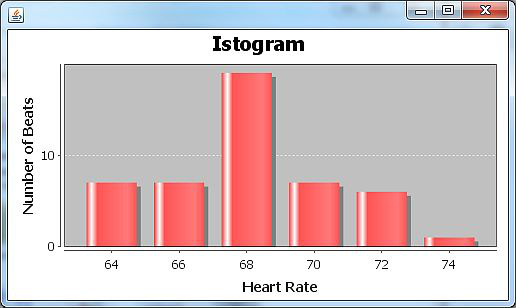
\includegraphics[width=90mm]{figures/ch5/1.png}
	\caption{Istogram from the desktop application resulted from an analysis on a MIT/BIH record.}
	\label{fig5.1}
\end{figure}
\begin{figure}[ht!]
	\centering
	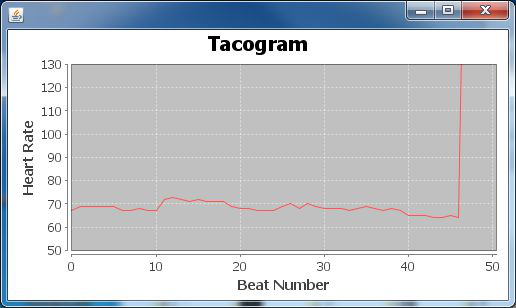
\includegraphics[width=90mm]{figures/ch5/2.png}
	\caption{Tacogram from the desktop application resulted from an analysis on a MIT/BIH record.}
	\label{fig5.2}
\end{figure}
\begin{figure}[ht!]
	\centering
	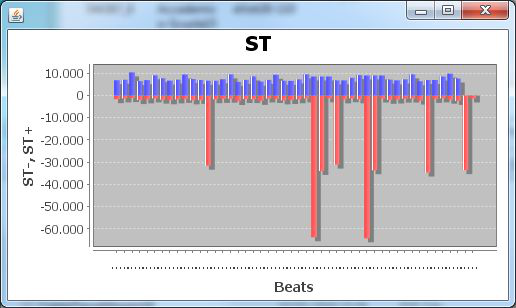
\includegraphics[width=90mm]{figures/ch5/3.png}
	\caption{ST+/ST- graph from the desktop application resulted from an analysis on a MIT/BIH record.}
	\label{fig5.3}
\end{figure}
\subsection{Highly parameterizable}
We believe in dynamic software, that is why we planned from the beginning on making this application dynamic. Even if the application is  build on top of the ZEcg standard, we plan to make the software responsive also to other standards. To achieve this, we planned to abstract all the acquisition device independent features and functionalities. In order to support as much as possible any variants of the original acquisition device, we plan to setup customizable parameters, the only related to the hardware implementation. With a little of changes the application will be able to interface with other devices as well for acquisition.
\section{Nonfunctional}
\subsection{Reduced memory usage}
This requirement is fundamental for any project related to mobile application development. In fact, if a desktop pc in general doesn’t have any problem related to memory usage (even if it is a good practice not to waste memory), on mobile devices this over-usage can bring the application to crash and get killed by the OS. The memory available is higher on new devices with respect to older ones,  but it is still small so it is always a good practice to use it carefully.
\subsection{Minimum performance rate and scalability on performance}
Nowadays the new high level mobile devices has quad-core or even octa-core cpu processors. Any application should take advantage of a such configuration, but on the other hand mobile application developers should always consider the fact that the market is still full of older and low-end devices. In order to cover at least most of the market devices their application have to run fine (with a minimum acceptable performance rate) starting from the low-end devices and, at the same time, taking advantage of last devices capabilities. \\
We believe modern applications should seriously take this aspect in consideration, because it will make their application scalable also from a performance point of view.
\subsection{ Wide platform compatibility and accessibility}
Developing a mobile application implies building a software that has to be executed on many different platforms. The smartphone and tablet market is huge with many different devices mounting different hardwares and running of the three major mobile OS (iOS, Android and Windows Phone). In the next chapters we will deal with this issue.   
\subsection{Documentation}
This thesis includes also a more technical documentation about the development phase and the choices we starting from the planning phase to the development phase. The software is fully documented and with annotations and comments to increase code readability and future development on top of it. The technical documentation is included in the next chapters where we are going to discuss and motivate the implementation and the results.
% Chapter 6

\chapter{Problems}
\label{Chapter6} 
By identifying  the requirements, we could then be able to highlight the related problems that we had to face in order to fulfill all of them. We will describe the related requirement as source of each faced problem.

\section{Mobile platform fragmentation}
Considering the requirement of a wide platform compatibility, we obviously need to face a really big problem in the mobile application world: the platform fragmentation.\\
Starting from the first smartphone release on 2007, the iPhone from Apple,  the sale of such devices keeps increasing each year. Between 2007 and 2008 sales proceeded upwards reaching the same sale rate of their computing parent, the PC. On 2009  the market signed an important inflection point, representing the beginning of an inexorable vertical rise. Although PCs were still the only ones to offer some types of functionality due to their longer replacement cycle, they were sold with a ratio of 1 : 2, compared to smartphones, over a 5 year period. This new market’ growth leads to an obvious seeking of various participants, some by choice and some by necessity, in order to extract value. Android has been the prime beneficiary, having been announced on 2007 and having gone on to account for well over half of smartphone sales worldwide. Apple, meanwhile, has maintained a steady ship, leveraging its skill in product design and user experience with a finely honed marketing machine, attracting a customer that rarely defects.\cite{ref5}
\begin{figure}[ht!]
	\centering
	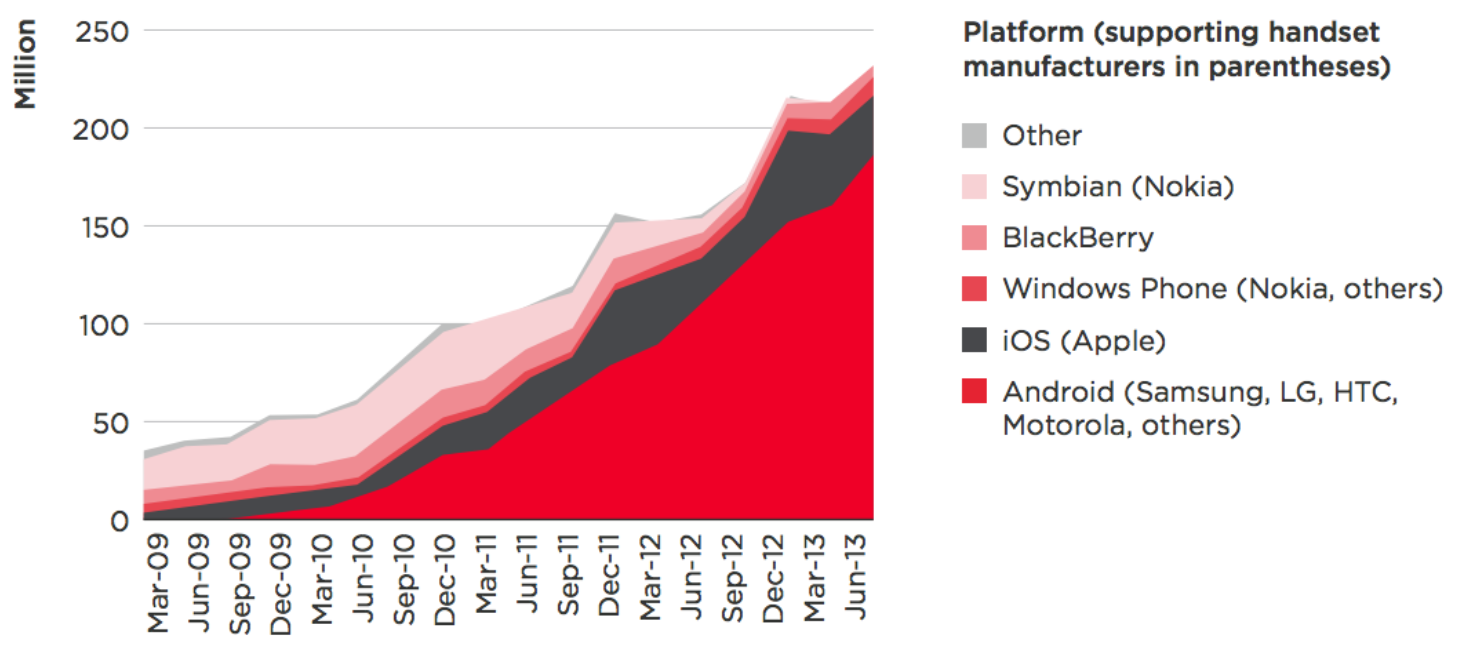
\includegraphics[width=120mm]{figures/ch6/1.png}
	\caption{Mobile platform share evolution (smartphone sales), 2009–13.}
	\label{fig6.1}
\end{figure}
Fast-forwarding to 2016, if we consider the global market share held by the leading smartphone operating systems, at first position we have Android with a share of  80.7\%, followed by iOS with a 17.7\%. Minor percentages are represented by Windows Phone (1.1\%), RIM (0.2\%) and others (0.2\%).\cite{ref6}

\section{Native vs Cross-Platform}
As mentioned earlier, one of the main challenges when moving to a mobile solution is the software development within a technology landscape that is highly fragmented and rapidly evolving. Mobile apps require a fair amount of customization to run on diverse platforms and a constant update due to the steady stream of new hardware, OS versions and browsers. Even a single platform (Android, Windows, Blackberry, and to a lesser extent Apple) has numerous flavors that require some degree of customization. There are also other factors such as the overlay software from different manufacturers that can affect behavior of an app on a particular device.\\
In response, the mobile industry has spawned a rapidly growing ecosystem of cross-platform and cross-device frameworks, source code analyzers, libraries of reusable components, and other tools designed to accelerate and simplify multi-platform development. New tools are constantly emerging, with new functionality, different capabilities,  strengths and weaknesses.\\
Developer’s preferences change and evolve, particularly as new tools and capabilities become available. However, the basic goals are the same: to code less and accomplish more, to reuse and recycle across multiple platforms as much as possible, and consider developing from scratch as the last resort. In addition, any tool or framework should be able to work with current and future evolving offers, and not to be locked because of a particular platform or technology.\cite{ref7}

% Chapter 7

\chapter{Solution choices}
\label{Chapter7}

After a long research period of time and direct experience on developing mobile application using the most known cross-platform (Xamarin) and hybrid (Cordova Phonegap) solution, we decided to go native. This decision was based mostly on the needs and the strict performance requirements related to the project. Thanks to a native implementation we can achieve better results in term of performance and in term of user experience of the application. At the choice of a native platform we picked  Android because it is the most spread mobile OS over mobile devices and it is open source even if mostly maintained by Google.

\section{Android Platform}
Android is a mobile operating system (OS) currently developed by Google, based on the Linux Kernel and designed primarily for touchscreen mobile devices such as smartphones and tablets. Android has the largest installed base of all operating systems of any kind. Android has been the best selling OS on tablets since 2013, and on smartphones it is dominant by any metric.\cite{ref18}
\begin{figure}[ht!]
	\centering
	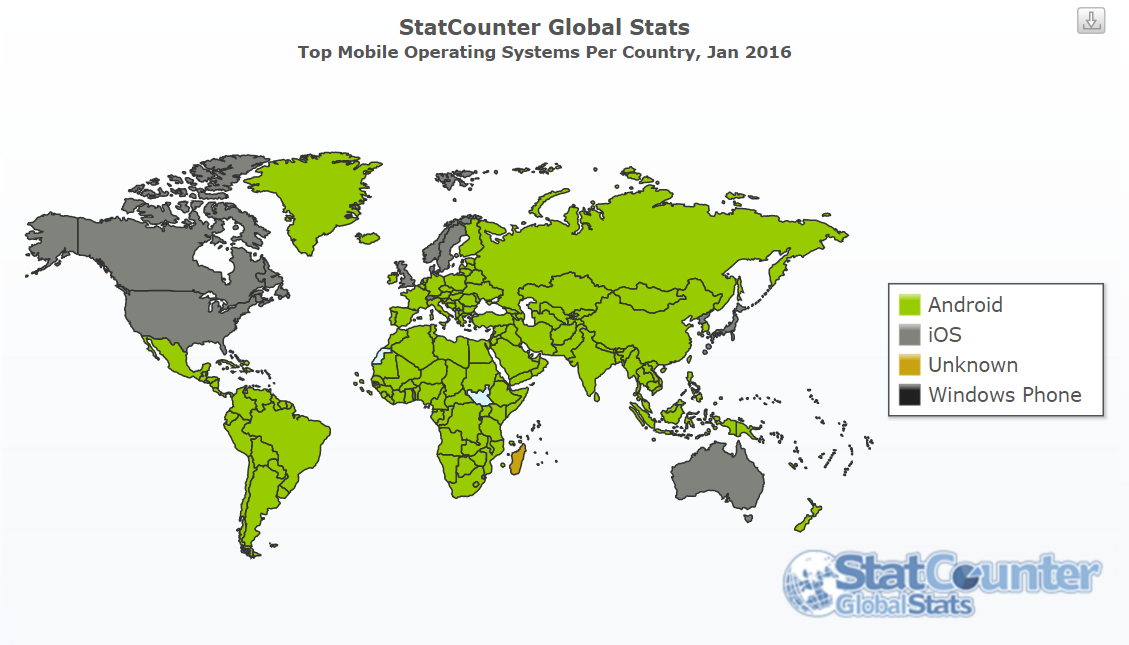
\includegraphics[width=120mm]{figures/ch7/1.png}
	\caption{Top Mobile Operating Systems Per Country, Jan 2016. Statcounter.com}
	\label{fig7.1}
\end{figure}
We have chosen to develop ECG-ira firstly on this platform because of it is widely spread over the world and its nature of being from an open source software made it stable and widely supported. The Android OS programming language is Java which is one of the most known and used OOP language for application and web development.

\section{Why native?}
The advantages of cross-platform (and hybrid) solution is mostly connected to code maintenance and to faster development, because most of the written codes stands for all the supported OS at building phase. Business logic and data structure can be easily share among the many OS for example by using Xamarin we can write unique code using C\# (c-sharp) and abstract the business logic, the web services and the database management independently from the specific platform we want to target.  Most of the time it is just a matter of working on different user interface, one for any supported OS. All of this look awesome and it is, but when it comes to performance metrics, custom interfaces and user experience, here we meet its weaknesses and limitations. ECG-ira main goal is to build up an usable and stable mobile medical application and to fulfill it we needed to exploit the native platform in order to achieve the best performance and the best user experience. As Android is the most spread mobile OS over smartphones and tablets it results in an obvious pick.\\
We believe native may not be the best pick for any kind of application. The choices has to be done according to the project requirements and goals. Pitfall for going native is the long development time and a deep (if not full) knowledge of that specific platform.

\section{Android concurrency exploitation}
As we have seen previously, a considerable computational effort is required to the app, especially during record acquisition. For this reason, the only way in order to guarantee a reasonable performance was to exploit the concurrency mechanisms available in the chosen platform. This decision will obviously increase the complexity of the execution: analyzing the execution of a single-threaded application is relatively simple because the order of execution is known. In multi-threaded applications, it is a lot more difficult to analyze how the program is executed and in which order the code is processed.\\
In the following paragraphs we will start from the basic mechanisms provided by Java language, and we will then analyse the ones, given available by the Android OS, that we have chosen to use in our application.

\subsection{Thread Overview}
Software programming is all about instructing the hardware to perform an action. The instructions are defined by the application code that the CPU processes in an ordered sequence, which is the high-level definition of a thread. From an application perspective, a thread is execution along a code path of Java statements that are performed sequentially. A code path that is sequentially executed on a thread is referred to as a task, a unit of work that coherently executes on one thread. A thread can either execute one or multiple tasks in sequence.

\subsubsection{Thread execution}
A thread in Java machine is represented by java.lang.Thread. It is the most basic execution environment in Android that executes tasks when it starts and terminates when the task is finished or there are no more tasks to execute; the alive time of the thread is determined by the length of the task. Thread supports execution of tasks that are implementations of the java.lang.Runnable interface. An implementation defines the task in the run method:
\begin{lstlisting}
	private class MyTask implements Runnable {
		public void run() {
			int i = 0; // Stored on the thread local stack.
		}
	}
\end{lstlisting}
All the local variables in the method calls from within a run() method—direct or indirect—will be stored on the local memory stack of the thread. The task’s execution is started by instantiating and starting a Thread:
\begin{lstlisting}
	Thread myThread = new Thread(new MyTask());
	myThread.start();
\end{lstlisting}
On the operating system level, the thread has both an instruction and a stack pointer. The instruction pointer references the next instruction to be processed, and the stack pointer references a private memory area—not available to other threads—where thread-local data is stored. Thread local data is typically variable literals that are defined in the Java methods of the application.\\
A CPU can process instructions from one thread at a time, but a system normally has multiple threads that require processing at the same time, such as a system with multiple simultaneously running applications. For the user to perceive that applications can run in parallel, the CPU has to share its processing time between the application threads. The sharing of a CPU’s processing time is handled by a scheduler. That determines what thread the CPU should process and for how long. The scheduling strategy can be implemented in various ways, but it is mainly based on the thread priority: a high-priority thread gets the CPU allocation before a low-priority thread and receive more execution time with respect to low-priority threads.\\
The execution of two concurrent threads can be done in java just declaring two Thread objects and then starting them by calling the method Thread .start():
\begin{lstlisting}
	Thread T1 = new Thread(new MyTask());
	T1.start();
\end{lstlisting}

\subsection{Threads in Android}
In Android there are basically three thread types:
\begin{itemize}
	\item \textbf{UI thread} (or main thread): it is started on application start and stays alive during the lifetime of the application process. The UI thread is the main thread of the application, used for executing Android components and updating the UI elements on the screen. If the platform detects that UI updates are attempted from any other thread, it will promptly notify the application by throwing a CalledFromWrongThreadException. This harsh platform behaviour is required because the Android UI Toolkit is not thread safe, so the runtime allows access to the UI elements from one thread only.
	\item \textbf{Binder threads}: they are used for communicating between threads in different processes. Each process maintains a set of threads, called a thread pool, that is never terminated or recreated, but can run tasks at the request of another thread in the process. These threads handle incoming requests from other processes, including system services, intents, content providers, and services.
	\item \textbf{Background threads}: All the threads that an application explicitly creates are background threads. This means that they have no predefined purpose, but are empty execution environments waiting to execute any task. The background threads are descendants of the UI thread, so they inherit the UI thread properties, such as its priority. By default, a newly created process does not contain any background threads. It is always up to the application itself to create them when needed.
\end{itemize}
The UI thread is the most important thread, but it gets no special scheduling advantage compared to the other threads—the scheduler is unaware of which thread is the UI thread. Instead, it is up to the application to not let the background threads interfere more than necessary with the UI thread.

\subsection{ Thread communication in Android}
In multithreaded applications, tasks can run in parallel and collaborate to produce a result. Hence, threads have to be able to communicate to enable true asynchronous processing.\\
The most common thread communication use case in Android is between the UI thread and worker threads. Hence, the Android platform defines its own message passing mechanism for communication between threads. The UI thread can offload long tasks by sending data messages to be processed on background threads. The message passing mechanism is a nonblocking consumer-producer pattern, where neither the producer thread nor the consumer thread will block during the message handoff.\\
The message handling mechanism in android is implemented with the following classes:
\begin{itemize}
	\item \textbf{android.os.Looper}: A message dispatcher associated with the one and only consumer thread.
	\item \textbf{android.os.Handler}: Consumer thread message processor and the interface for a producer thread to insert messages into the queue. A Looper can have many associated handlers, but they all insert messages into the same queue.
	\item \textbf{android.os.MessageQueue}: Unbounded linked list of messages to be processed on the consumer thread. Every Looper—and Thread—has at most one MessageQueue.
	\item \textbf{android.os.Message}: Message to be executed on the consumer thread.
\end{itemize}
	The mechanism is summarized in the figure \ref{fig7.2}.
\begin{figure}[ht!]
	\centering
	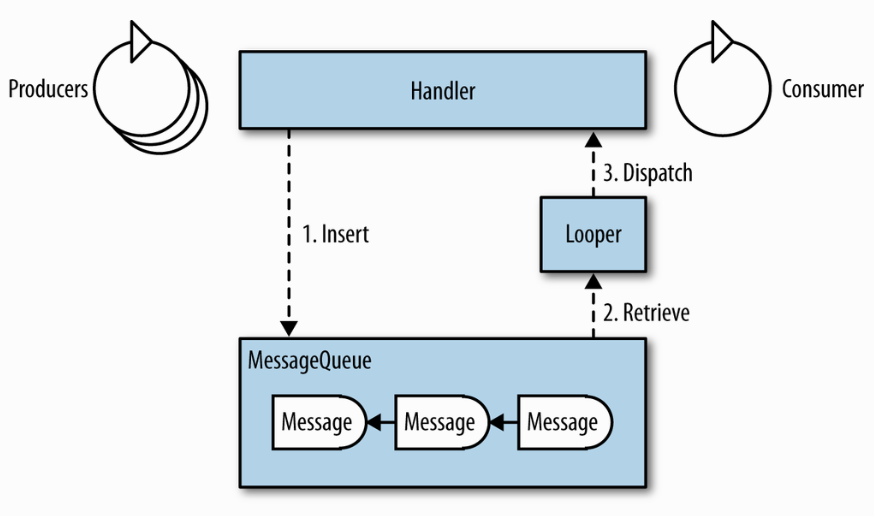
\includegraphics[width=120mm]{figures/ch7/2.png}
	\caption{Overview of the message-passing mechanism between multiple producer threads and one consumer thread.}
	\label{fig7.2}
\end{figure}
\begin{itemize}
	\item \textbf{Insert}: The producer thread inserts messages in the queue by using the Handler connected to the consumer thread.
	\item \textbf{Retrieve}: The Looper runs in the consumer thread and retrieves messages from the queue in a sequential order.
	\item \textbf{Dispatch}: The handlers are responsible for processing the messages on the consumer thread. A thread may have multiple Handler instances for processing messages; the Looper ensures that messages are dispatched to the correct Handler.
\end{itemize}

\subsection{HandlerThread}
Now we will describe a component that we have heavily exploited in our application, and as you will see in implementation details section, it represents the base of two main operations: the ECG signal drawing during both acquisition and record opening, and the ECG signal reading during record opening.\\
HandlerThread is a thread with a message queue that incorporates a Thread, a Looper, and a MessageQueue. It is constructed and started in the same way as a Thread. Once it is started, HandlerThread sets up queuing through a Looper and MessageQueue and then waits for incoming messages to process:
\begin{lstlisting}
	HandlerThread handlerThread = new HandlerThread("HandlerThread");
	handlerThread.start();
	
	mHandler = new Handler(handlerThread.getLooper()) {
		@Override
		public void handleMessage(Message msg) {
			super.handleMessage(msg);
			// Process messages here
		}
	};
\end{lstlisting}
There is only one queue to store messages, so execution is guaranteed to be sequential, and therefore thread safe. The HandlerThread sets up the Looper internally and prepares the thread for receiving messages.\\
Here is a simple example of an implementation:
\begin{lstlisting}
        public class MyHandlerThread extends HandlerThread {
	        private Handler mHandler;
	        public MyHandlerThread() {
		        super("MyHandlerThread", Process.THREAD_PRIORITY_BACKGROUND);
	        }
	        @Override
	        protected void onLooperPrepared() {
		        super.onLooperPrepared();
		        mHandler = new Handler(getLooper()) {
			        @Override
			        public void handleMessage(Message msg) {
				        switch(msg.what) {
								case 1:
						        // Handle message
						        break;
					        case 2:
						        // Handle message
						        break;
				        }
				    }
			    };
	        }
	        public void publishedMethod1() {
		        mHandler.sendEmptyMessage(1);
	        }
	        public void publishedMethod2() {
		        mHandler.sendEmptyMessage(2);
	        }
        }
\end{lstlisting}

\subsubsection{Lifecycle}
A running HandlerThread instance processes messages that it receives until it is terminated. A terminated HandlerThread can not be reused. To process more messages after termination, create a new instance of HandlerThread. The lifecycle can be described in a set of states:
\begin{itemize}
	\item \textbf{Creation}: The constructor for HandlerThread takes a mandatory name argument and an optional priority for the thread:
	\begin{lstlisting}
		HandlerThread(String name)
		HandlerThread(String name, int priority)
	\end{lstlisting}
	The name argument simplifies debugging, because the thread can be found more easily in both thread analysis and logging. The priority argument is optional and should be set with the same Linux thread priority values used in Process.setThreadPriority. The default priority is Process.THREAD\_PRIORITY\_DEFAULT, the same priority as the UI thread, and can be lowered to Process.THREAD\_PRIORITY\_BACKGROUND to execute non-critical tasks.
	\item \textbf{Execution}: The HandlerThread is active while it can process messages; i.e., as long as the Looper can dispatch messages to the thread. The dispatch mechanism is set up when the thread is started through HandlerThread.start and it is ready when either HandlerThread.getLooper returns or on the onLooperPrepared callback. A HandlerThread is always ready to receive messages when the Handler can be created, as getLooper blocks until the Looper is prepared.
	\item \textbf{Reset}: The message queue can be reset so that no more of the queued messages will be processed, but the thread remains alive and can process new messages. The reset will remove all pending messages in the queue, but not affect a message that has been dispatched and is executing on the thread:
	\begin{lstlisting}
		public void resetHandlerThread() {
			mHandler.removeCallbacksAndMessages(null);
		}
	\end{lstlisting}
	The argument to removeCallbacksAndMessages removes the message with that specific identifier. null, shown here, removes all the messages in the queue.
	\item \textbf{Termination}: A HandlerThread is terminated either with quit or quitSafely, which corresponds to the termination of the Looper. With quit, no further messages will be dispatched to the HandlerThread, whereas quitSafely ensures that messages that have passed the dispatch barrier are processed before the thread is terminated. You can also send an interrupt to the HandlerThread to cancel the currently executing message:
	\begin{lstlisting}
		public void stopHandlerThread(HandlerThread handlerThread) {
			handlerThread.quit();
			handlerThread.interrupt();
	  }
	\end{lstlisting}
	A terminated HandlerThread instance has reached its final state and it cannot be restarted.
\end{itemize}

\subsection{Thread Pools}
A thread pool is the combination of a task queue and a set of worker threads that forms a producer-consumer setup. Producers add tasks to the queue and worker threads consume them whenever there is an idle thread ready to perform a new background execution. Therefore, the worker thread pool can contain both active threads executing tasks, and idle threads waiting for tasks to execute.
There are several advantages with thread pools over executing every task on a new thread (thread-per-task pattern):
\begin{itemize}
	\item The worker threads can be kept alive to wait for new tasks to execute. This means that threads are not created and destroyed for every task, which compromises performance.
	\item The thread pool is defined with a maximum number of threads so that the platform is not overloaded with background threads—that consume application memory—due to many background tasks.
	\item The lifecycle of all worker threads are controlled by the thread-pool lifecycle.
\end{itemize}

\subsubsection{ThreadPoolExecutor}
A thread pool’s behaviour is based on a set of properties concerning the threads and the task queue, which you can set to control the pool. The properties are used by the ThreadPoolExecutor to define thread creation and termination as well as the queuing of tasks. The configuration is done in the constructor,
\begin{lstlisting}
	ThreadPoolExecutor executor = new ThreadPoolExecutor(
	int corePoolSize,
	int maximumPoolSize,
	long keepAliveTime,
	TimeUnit unit,
	BlockingQueue<Runnable> workQueue);
\end{lstlisting}
where:
\begin{itemize}
	\item \textbf{corePoolSize}: The lower limit of threads that are contained in the thread pool. Actually, the thread pool starts with zero threads, but once the core pool size is reached, the number of threads does not fall below this lower limit. If a task is added to the queue when the number of worker threads in the pool is lower than the core pool size, a new thread will be created even if there are idle threads waiting for tasks. Once the number of worker threads is equal to or higher than the core pool size, new worker threads are only created if the queue is full.
	\item \textbf{maximumPoolSize}: The maximum number of threads that can be executed concurrently. Tasks that are added to the queue when the maximum pool size is reached will wait in the queue until there is an idle thread available to process the task.
	\item \textbf{keepAliveTime}: Idle threads are kept alive in the thread pool to be prepared for incoming tasks to process, but if the alive time is set, the system can reclaim noncore pool threads. The alive time is configured in TimeUnits, the unit the time is measured in.
	\item \textbf{workQueue}: An implementation of BlockingQueue that holds tasks added by the consumer until they can be processed by a worker thread. Depending on the requirements, the queuing policy can vary.
\end{itemize}

\subsubsection{ScheduledThreadPoolExecutor}
This is an extension of the ThreadPoolExecutor, which can schedule commands to run after a given delay, or to execute periodically. This class will be really useful in our application because of its capability of scheduling task at a fixed rate through the method:
\begin{lstlisting}
	scheduleAtFixedRate(Runnable command, long initialDelay,
		long period, TimeUnit unit)
\end{lstlisting}
where:
\begin{itemize}
	\item \textbf{command}: the task to execute
	\item \textbf{initialDelay}: the time to delay first execution
	\item \textbf{period}: the period between successive executions
	\item \textbf{unit}: the time unit of the initialDelay and period parameters
\end{itemize}

\subsection{AsyncTask}
As the name indicates, an AsyncTask is an asynchronous task that is executed on a background thread. The only method you need to override in the class is doInBackground(). Hence, a minimal implementation of an AsyncTask looks like this:
\begin{lstlisting}
	public class MinimalTask extends AsyncTask {
		@Override
		protected Object doInBackground(Object... objects) {
			// Implement task to execute on background thread.
		}
	}
\end{lstlisting}
The task is executed by calling the execute method, which triggers a callback to doInBackground on a background thread:
\begin{lstlisting}
	new MinimalTask().execute(Object... objects);
\end{lstlisting}
When an AsyncTask finishes executing, it cannot be executed again—i.e., execute is a one-shot operation and can be called only once per AsyncTask instance, the same behaviour as a Thread.\\
In addition to background execution, AsyncTask offers a data passing mechanism from execute to doInBackground. Objects of any type can be passed from the initiating thread to the background thread. This is like HandlerThread, but with AsyncTask you do not have to be concerned about sending and processing Message instances with a Handler.\\
In the common case where you want to execute a task in the background and deliver a result back to the UI thread, AsyncTask shines; it is all about handling the flow of preparing the UI before executing a long task, executing the task, reporting progress of the task, and finally returning the result. All of this is available as optional callbacks to subclasses of the AsyncTask, which look like this:
\begin{lstlisting}
	public class FullTask extends AsyncTask<Params, Progress, Result> {
		@Override
		protected void onPreExecute() { ... }
		@Override
		protected Result doInBackground(Params... params) { ... }
		@Override
		protected void onProgressUpdate(Progress... progress) { ... }
		@Override
		protected void onPostExecute(Result result) { ... }
		@Override
		protected void onCancelled(Result result) { ... }
	}
\end{lstlisting}
This implementation extends the AsyncTask and defines the arguments of the objects that are passed between threads:
\begin{itemize}
	\item \textbf{Params}: Input data to the task executed in the background.
	\item \textbf{Progress}: Progress data reported from the background thread (i.e. from doInBackground) to the UI thread in onProgressUpdate.
	\item \textbf{Result}: The result produced from the background thread and sent to the UI thread.
\end{itemize}
All callback methods are executed sequentially, except onProgressUpdate, which is initiated by and runs concurrently with doInBackground. Figure \ref{fig7.3} shows the lifecycle of an AsyncTask and its callback sequence.
\begin{figure}[ht!]
	\centering
	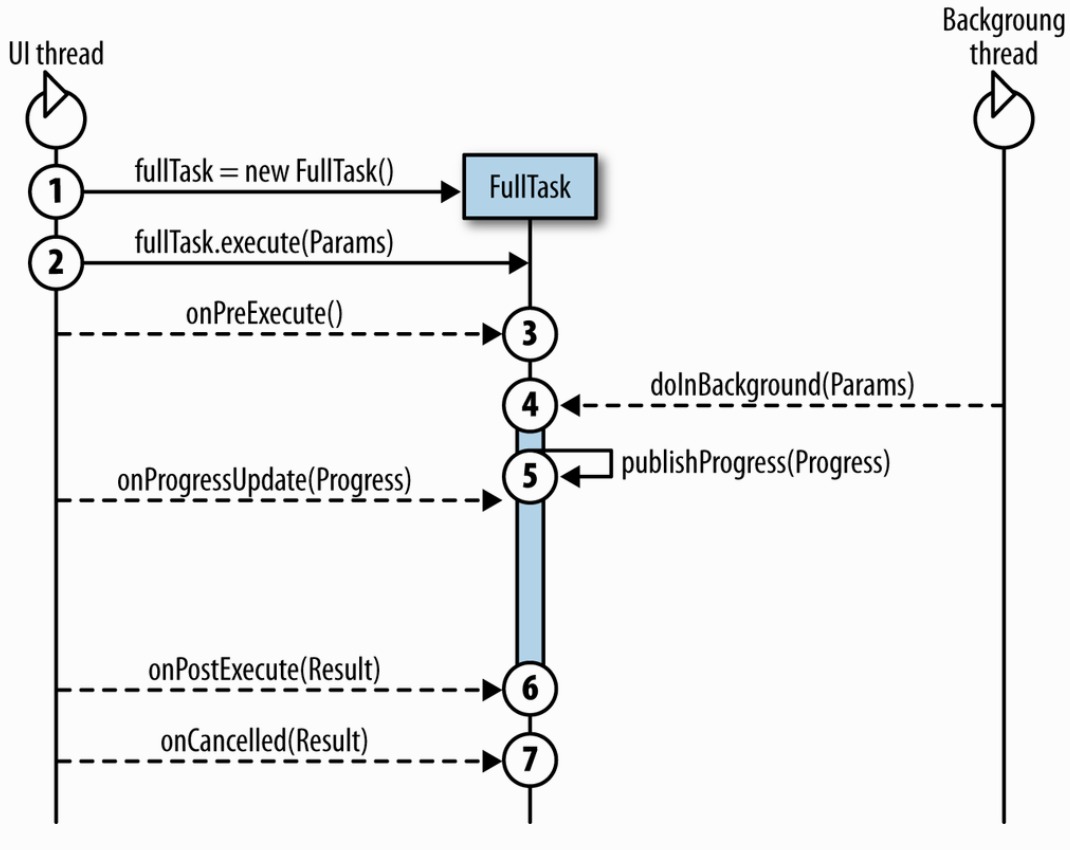
\includegraphics[width=120mm]{figures/ch7/3.png}
	\caption{The execution lifecycle of AsyncTask.}
	\label{fig7.3}
\end{figure}
The different steps are:
\begin{enumerate}
	\item Create the AsyncTask instance.
	\item Start execution of the task.
	\item First callback on the UI thread: onPreExecute. This usually prepares the UI for the long operation—e.g., by displaying a progress indicator on the screen.
	\item Callback on a background thread: doInBackground. This executes the long-running task.
	\item Report progress updates from the publishProgress method on the background thread. These trigger the onProgressUpdate callback on the UI thread, which typically handles the update by changing a progress indicator on the screen. The progress is defined by the Progress parameter.
	\item The background execution is done and is followed by running a callback on the UI thread to report the result. There are two possible callbacks: onPostExecute is called by default, but if the AsyncTask has been cancelled, the callback onCancelled gets the result instead. It is guaranteed that only one of the callbacks can occur.
\end{enumerate}
The progress update mechanism solves two use cases:
\begin{itemize}
	\item Displaying to the user how the long-running operation is progressing, by continuously reporting how many of the total tasks are executed.
	\item Delivering the result in portions, instead of delivering everything at the end in onPostExecute. For example, if the task downloads multiple images over the network, the AsyncTask does not have to wait and deliver all images to the UI thread when they are all downloaded; it can utilize publishProgress to send one image at the time to the UI thread. In that way, the user gets a continuous update of the UI.\cite{ref19}
\end{itemize}

\section{Baseline wander solutions}
In order to solve this problem, taking into account all the related problematic, we have chosen two kinds of approach. Each one will be described afterwards. The first approach will be always active, and will consist in the dynamic calculation of samples vertical axis during drawing iteration. The second is the usage of a simple moving average filter that could be activated in the app settings for the acquisition phase.

\subsection{Adaptive vertical displaying}
We decided to hold this type of solution active by default in order to maintain a solid and versatile way to overcome the worst scenario caused by a strong baseline wander. The approach works like this: at each frame drawing, we have a visible window of samples, with a length dictated from the space available on the device's screen, that we have to plot. Given that window, we know that we have to fit as many samples as we can, inside the space dedicated to that signal, the signal ECG strip. In a normal scenario, the signal will be aligned to a baseline, and so we can easy plot all the samples inside the relative strip. However in some other scenarios, it could happen that because of movement of the patient, the signal could immediately drop down. For this reason, the signal could easily go out of the available vertical space. To avoid this, we have to provide a mechanism in order to hit these cases and accordingly respond. We do this by not fixing the vertical baseline of the ECG strip, and leave it dynamic. Therefore this baseline will go up and down according to the position of the values inside the samples window. So every time, before we redraw the updated window on the screen, we compute the baseline of the signal at that moment by computing the mean of all samples. After that, we can shift the signal to plot up or down, trying to include the majority of samples on the screen. An example of the mechanism is showed in the figure \ref{fig7.4}. As you can see, starting from the second 23, a patient movement caused the baseline wander artifact, causing a drop of the D1 signal. The app by applying the dynamic displaying, it computed the new baseline of the signal, represented by the mean of all samples, and shifted all sample window accordingly. In the figure, the variation of the vertical axis is represented by $\Delta y$.\\
In this way we can overcome this type of scenario, avoiding the appliance of any kind of filtering. The latter, depending on the technique, can result in some percentage of error on the filtered ECG signal.
\begin{figure}[ht!]
	\centering
	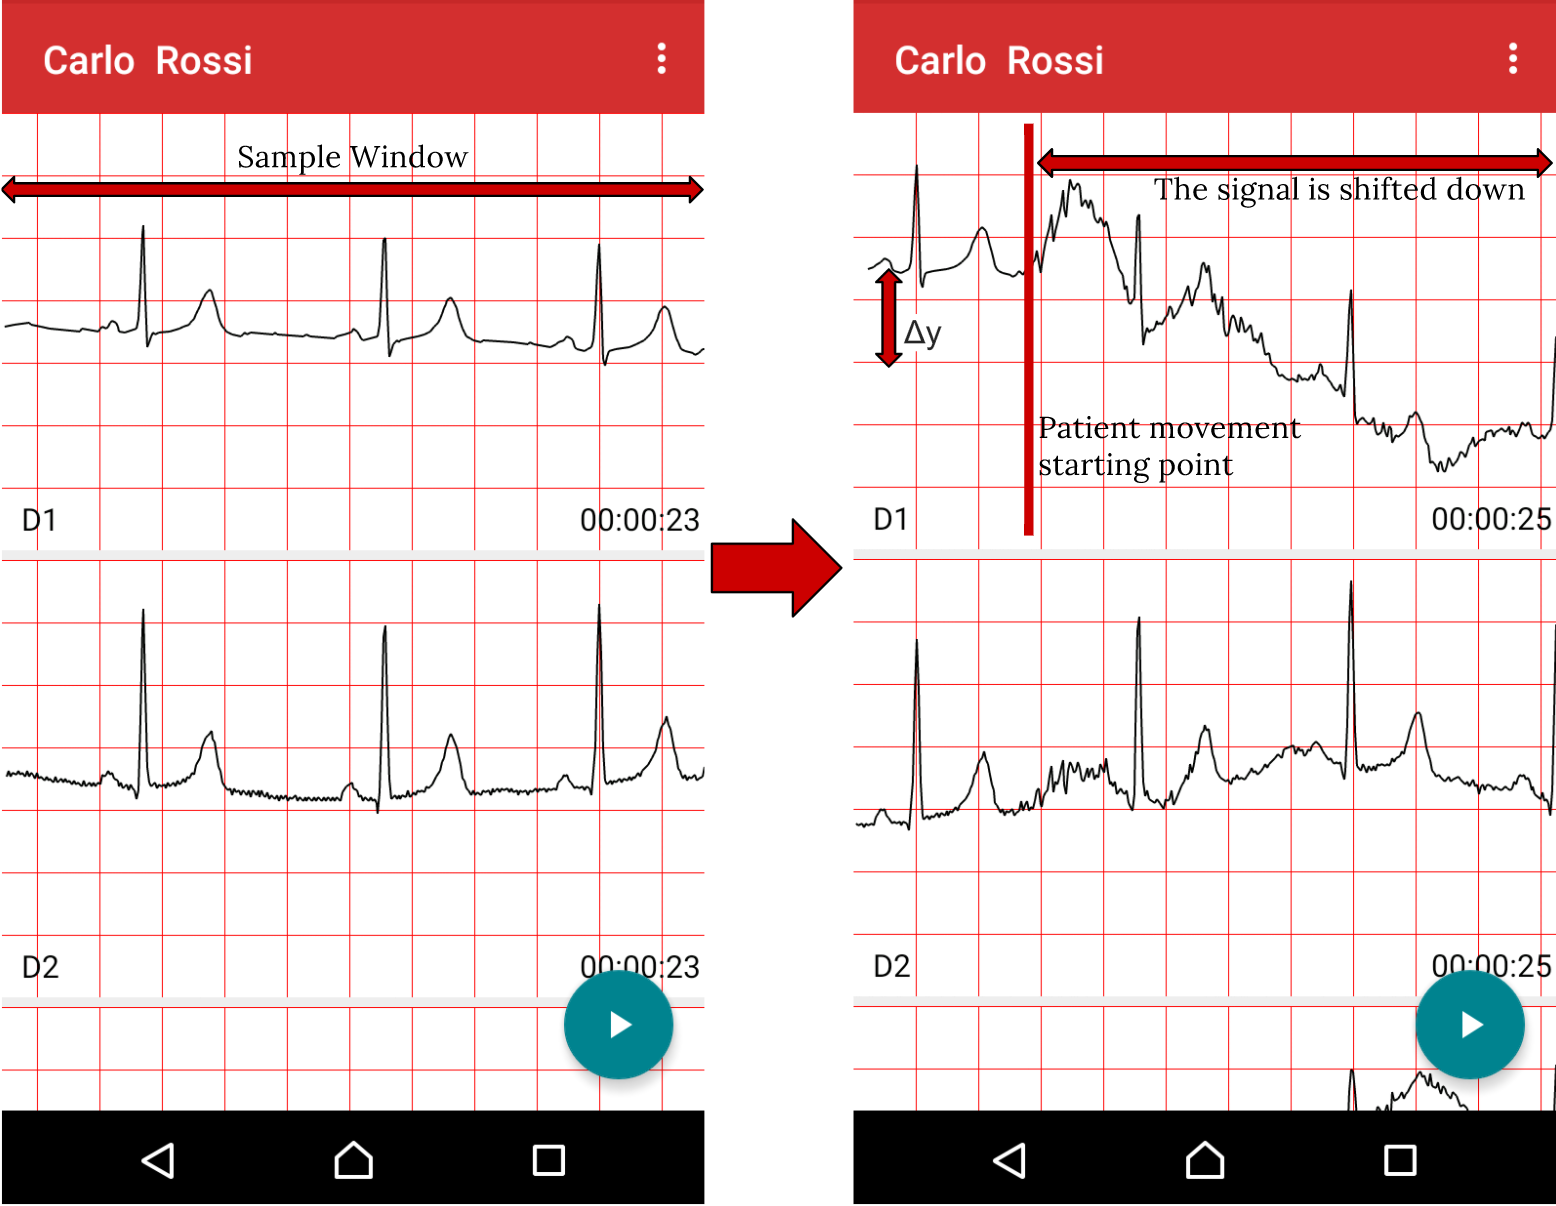
\includegraphics[width=130mm]{figures/ch7/4.png}
	\caption{The dynamic displaying result after a patient movement, causing the baseline wander artifact.}
	\label{fig7.4}
\end{figure}

\subsection{Moving average filter}
As discussed in the requirements section, many types of filtering are known to overcome to the baseline wander artifact. Some of them are capable to reduce at minimum the error on the output signal. Nevertheless this comes with a cost in computational effort, and so there is the need to mediate between the type of filtering and its related complexity.
Unfortunately in our case, putting in all the required operation, especially during real-time acquisition, where the app has to hold the bluetooth channel for transmission, interpret the transmitted signal, write to a file, derive the missing ECG lead, and plot at a reasonable rate the acquired signal, we had very limited computational availability to spend in any type of filtering in order to remove the eventual baseline wander. Therefore we decided to apply the most basic type of filtering during acquisition that is the simple moving average filtering. Given that, we are conscious about the possible distortion introduced by this filter, that's why we decided to:
\begin{itemize}
	\item Take a reasonable size for the moving average window (two seconds at least), inasmuch if it is true that as much as the window size grows, the effectiveness of the filter decreases, by doing this, we can keep the error rate low.
	\item Keep the filter deactivated by default, so that the doctor will decide when will be opportune to use it.
\end{itemize}

\section{Custom View Drawing}
Now we will talk about the most costly operation performed about our application. This was the thing on which we have spent lots of work, investigating all the problematic and different possibilities that we had in order to make the best possible implementation choice. We have mentioned earlier the computational effort that needs to be spent on signal drawing and for this reason we tried all the possible ways in order to discard the bad implementation, always having performance in our mind.

\subsection{Custom Libraries}
This was our first trial: we tried to find some libraries that could have permitted us to avoid an implementation from scratch of our drawing classes. For sure this possibility was the easiest possible. Given that our signal was not so different from other types of signals, as could be interpreted as a generic function plotted on a two dimensional system, we had quite sure that we could have found a nice plotting library and avoid useless implementation. Actually, we were able to find some well-realized libraries for handling plottings, but all of them clashed with one characteristic that we was seeking for: the customization of the rendered views, as we have said previously, has to mimic as much as possible the ECG paper on the look and also respect the required standard sizing of the same. Therefore, for this reason, we needed to discard this solution, given that some libraries permitted us to have very good displaying performance.

\subsection{Hardware Accelerated Drawing (GPU)}
Another solution, and potentially the best one, was to exploit the graphic hardware acceleration. Android is possible by using OpenGL ES, a subset of the OpenGL API designed for embedded system. The use of OpenGL can move all the graphics computations to the GPU, and so freeing up precious computing resources on the CPU. But unfortunately, in Android the usage of these libraries is not so integrated: they are written in hardware native code, which is C. This characteristic, while could of course guarantee the best performance\cite{ref20}, introduce a misalignment with the language used for developing Android application, which is Java. As a result, it is a common belief that the usage of OpenGL ES in Android is quite painful, forcing many developers to switch to better alternative libraries and frameworks, like Unity, LibGDX, Cocos2D or others. Putting aside all the problematic related to its implementation's effort, we decided to try OpenGL ES for the drawing part. With much surprise, this led us to an unexpected result: the results in performances were quite beneath the performance achieved using the CPU also for the application drawing. This relies on the fact that, as said earlier, the OpenGL libraries on Android are not so integrated, and developer are required to represent datatypes of the C language in the Java language. This may not seem problematic, but in a situation where all ECG samples need to be represented as classes, holding their coordinates in the ECG paper space in a corresponding matrix, and at each draw update there is the need to reallocate all the samples matrix, causing a remapping to the C data types, the performance improvements  are quickly drop out. For this reason, we realized that our best chance was to relying on the CPU also for the drawing, and trying as much as possible to optimize the algorithms in order to achieve the best performances.

\subsection{Not hardware Accelerated Drawing (CPU)}
Having underlined the downsides of the previous solution, we decided to spend all our energies to implement the best possible drawing code, relying on the mechanisms provided by Android for drawing operations using the CPU. This is possible using Canvas.\\
Android Canvas provides the developer with the ability to create and modify 2D images and shapes. Moreover, the Canvas can be used to create and render our own 2D objects as this class provides various drawing methods to do so. Canvas can also be used to create some basic animations such as frame-by-frame animations or to create certain Drawable objects such as buttons with textures and shapes such as circles, ovals, squares, polygons, and lines.\cite{ref21}\\
As we mentioned in the chapter about Android concurrency exploitation, all applications run on a single thread in Android. All instructions run in a sequence on the UI thread, meaning that the second instruction will not start unless the first one is finished. The UI thread as it is responsible for drawing all the objects or views on the screen and processing all events, such as screen touches and button clicks. Now the problem is that, if we have two operations scheduled to run in the same default thread or UI thread and the first operation takes too long to finish, the system will ask the user to forcibly close the application or wait for the process to complete. This scenario is called ANR (Application Not Responding).\\
Given that we wanted also to provide scrolling of the different ECG leads in our app, we could not hold this computational effort on the UI thread, which as result of drawing operations, would be blocked. Therefore we decided to assign all the drawing operations on different threads created ad-hoc. The number of threads dedicated to drawing will be decided at run time by the application, depending on the device availability, and thus allowing device scalability.\\
The use of Canvas permitted us to achieve both reasonable performances, after a deep code optimization, and high customization of the rendered view.
%Chapter8
\chapter{System architecture}
\label{Chapter8}
The entire system is based on an acquisition device named ZEcg, and a native mobile application on the Android Platform. Our focus and main effort were on the developing of the mobile application fulfilling all the requirements. The acquisition device was instead developed and designed by Crespi Alessandro and Ulisse Pizzagalli during their thesis work at the Politecnico of Milan.~\cite{ref22}
\section{Acquisition device}
ZEcg is composed by the following different modules:
\begin{enumerate}
	\item OVP: used to protect the patient from high voltage or voltage leakage.
	\item LFP EMI Filter: anti-aliasing RC filter used to remove noises due to high frequencies.
	\item RLD: Active electrode driver for the right leg
	\item WCT: Derivator used to compute the precordials (Wilson Central Terminator)
	\item PGA: 8 gain amplifier with programmable inputs
	\item ADC: 8 analog-digital 16 bit 8KSa/s converter.
	\item MCU: microcontroller
	\item Bluetooth: bluetooth module for data transmission
	\item Power MGMT: to manage battery recharge and stabilizer
\end{enumerate}
\begin{figure}[ht!]
	\centering
	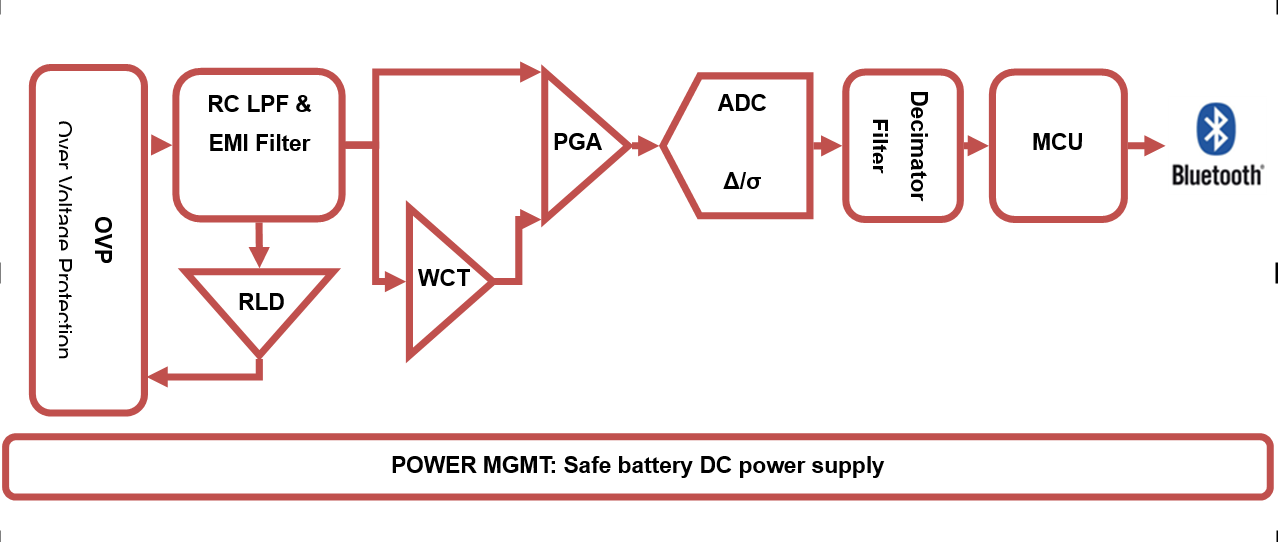
\includegraphics[width=110mm]{figures/ch8/1.png}
	\caption{ZEcg device block diagram including all the modules components.}
	\label{fig8.1}
\end{figure}
The core component is the Texas Instrument system on chip ADS1198. This chip has 8 input bipolar channels, representing the 8 clinical leads.\\
The channels 1 and 2 produce the lead I and lead II. Channel 1 measures the potential difference between the electrode RA(-) and the electrode LA(+), the channel 2 the difference between RA(-) and LL(+). Lead III and the augmented leads are obtained from a combination of lead I and lead II at software level.\\
V1, V2,...,V6 are computed as difference between the respective electrode and the signal related to the negative value of the WCT (Wilson Central Terminator).\\
The WCT signal comes from the average between RA, LA and LL and it's connected to the channels 3,4,5,6,7,8.
\begin{figure}[ht!]
	\centering
	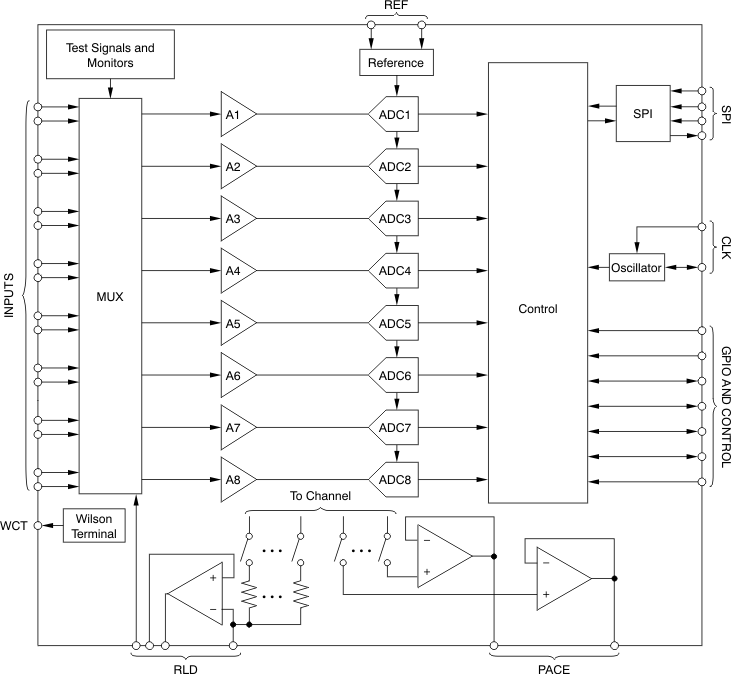
\includegraphics[width=120mm]{figures/ch8/2.png}
	\caption{ADS1198 functional diagram showing the 8 channels representing the 8 leads used during the ECG record acquisition.}
	\label{fig8.2}
\end{figure}
Each channel is amplified using a programmable gain (PGA) and a CMRR, before being converted into digital. For more details about the entire device architecture we invite you to read the thesis of our colleagues Crespi Alessandro and Ulisse Pizzagalli\cite{ref22} who designed and developed ZEcg.
\subsection{Mobile app}
The mobile application we developed for this thesis work was implemented having in mind all the user best interface design principles and the best practice starting from the planning and design phase to the final  coding phase. As this application was designed for Android OS, we strictly followed Google specific standards and procedures.\\
We made use of Android Studio as IDE (strongly suggested by Google as main IDE to develop Android native applications). Starting from 2013 the development of native Android application moved from Eclipse + Android Plugin to Android Studio. The entire project building system has changed and moved to use the Gradle  building system\cite{ref23}. 
The entire process during project building to compilation can be resumed in the following image:
\begin{figure}[ht!]
	\centering
	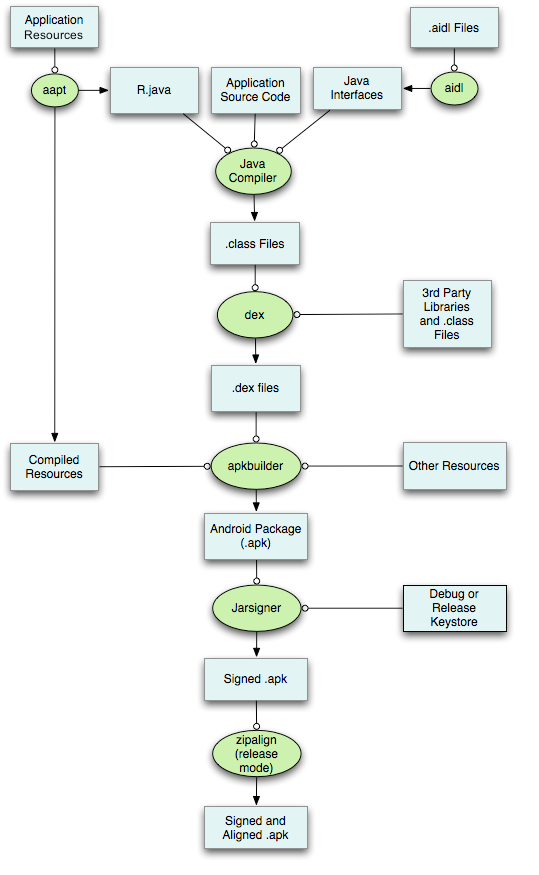
\includegraphics[width=90mm]{figures/ch8/3.png}
	\caption{Android Build system process. How and which component are involved during an android application build and compilation.}
	\label{fig8.3}
\end{figure}
The most important steps along the building process are:
\begin{enumerate}
	\item The Android Asset Packaging Tool (aapt) takes the application resource files, such as AndroidManifest.xml file and the XML files for the Activities, and compiles them. A R.java  file is produced so that all the resources can be easily accessed within your application.
	\item The aidl tool converts any .aidl interfaces into Java interfaces.
	\item The Java compiler will compile the R.java and .aidl files generating the .class files.
	\item The Dex tool will convert the .class files to Dalvik bytecode. Any third libraries and .class files included in the project build will be also converted into .dex files so that they can be later packed into the final .apk.
	\item All non-compiled resources(such as images), compiled resources, and the .dex files  are sent to the apkbuilder tool that will output the .apk file.
	\item Once the .apk is built, it must be signed with either a debug or release key before it can be installed to a device.
	\item To reduce the size of the .apk and to decrease the memory usage for releasing mode the zipalign tool is launched.
\end{enumerate}
We split the application functionalities into different packages. 
\begin{figure}[ht!]
	\centering
	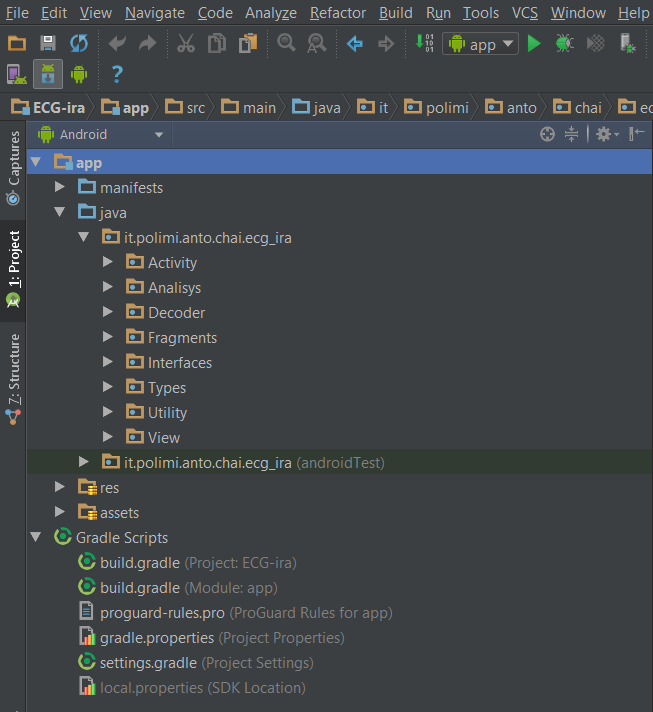
\includegraphics[width=90mm]{figures/ch8/4.png}
	\caption{ECG-ira project structure and packages inside Android Studio IDE.}
	\label{fig8.4}
\end{figure}
The packages content are divided as follow:
\begin{itemize}
	\item Activity: it contains all the Activity used inside the Application.
    \item Analysis: All the java classes used for the analysis of the ECG records; they include the Neural Network, the QRSDetector, the PWaveDetector and some signal Filters implementations.
	\item Decoder:  this package contains the java classes in charge to decode and parse the .hea and .dat files.
	\item Fragments: contains some fragments used inside the application, for example  the ones used to show the chronograms (Istogram, Tacogram, ST graphs).
	\item Interfaces: all interfaces declarations to abstract the specific application behaviour with more general one.
	\item Utility: some utility class such as the in application FileManager.java class, and the Adapters used within the application (for example to show ListViews or RecycleViews).
	\item View: it contains all the classes working directly on the View and the custom view themselves such as the View used to show the ECG grid.
\end{itemize}
The key points of this application are based on three main concepts:
\begin{itemize}
	\item Code reuse and maintainability
	\item Maximize performance depending on the device constraints (CPU, memory, storage capacity)
	\item Usability in term of interface and interaction
\end{itemize}
\subsubsection{Code reuse and maintainability}
The most important classes representing the core of the application functionalities are all abstracted through interfaces or in case of the classes related to the View through a set of parameters. This makes the application highly customizable and easily to extend. For example if in a next future there will be a new ECG data format, it can be possible to give the app the capability to read and parse such a format just by implementing the interfaces and writing the specific code to parse such a new data format.\\
A concrete example is given in our code by observing that both the MITDatReader and the ZEcgDatReader extends the abstract class DatReader, so the next format reader has just to extend it as well. We know that MIT-BIH format is completely different from the ZEcg format, that why specific code to parse the file content to extract the signal is mandatory.\\
Any new format reader has just to override the method:
\begin{lstlisting}
public void readAndAddSample(int numOfSample, int addPosition) {
}
\end{lstlisting}
More concrete details about the effective implementation will be exploited later on in the next chapters.
\subsubsection{Maximize performance depending on the device constraints}
We do well know about the great number of constraints due to the huge number of different devices with different hardware on. We decide to make our application available starting from Android API 16 (the minimum sdk API recommended by Google to support).  To overcome the problem of the difference devices and Android OS version starting from Jelly Bean (API 16) we took maximum advantages from the device hardware by splitting the thread jobs in between the maximum number of cores available. In the class CpuInfoExtractor we discover the hardware capabilities (number of cores) and according to it we split the calculus between a certain number of threads. More the cores, more the threads we can take advantage of.\\
From an interface point of view instead, we are forced  to depend on the density of pixel of the device screen and its size, but at the same time to accomplish our requirements related to achieve a perfect grid of squares of centimeters. We found a way to always achieve the same dimensions of square independently by the screen size of the devices by retrieving and taking in account the display exact pixels per inch size in the X dimension. Then, we computed the number of pixels needed to achieve the right sizing.  In this way, we solved the problem of having same dimensions and so metrics on different devices. On the other hand, if this method is quite functional and device independent, on devices with different screen size (width for example) the number of grid cells may vary from just a few on small screen, to many of them on tablets. This is a direct consequence due to the difference in number of pixels and the pixels size itself (some are squared but most of them are rectangles).\\

\subsubsection{ Usability in term of interface and interaction}
One mobile application is usable if it does what the user expects it to do when interacting with it.\\
We followed all Google guidelines in term of user experience using native view and patterns. We took advantage of the last API features, such as RecycleViews instead of the old classic ListViews. We made use of the button ripple effects available starting from Lollipop (Android API 21), but at the same time we provided to the older Android OS version the selector effect that still gives a nice response to the user interaction with command and buttons. We made use of the typical android Preference Settings so familiar to Android users and most important we always inform the user about the operations going on so he never feels lost inside the application.
% Chapter 9

\chapter{Implementation details}
\label{Chapter9}

In this chapter we will focus on the implementation details of the main components and operation, trying to give a clearer idea of the mechanism under the hood of the app. We will start by explaining the general idea and purpose of each included component and their main functions. Then we will move to the sequence flow section, where we will put all pieces together in order to explain their iterations and give a picture of what is happening in the different use cases.

\section{Main components}
We decided to include only, which are for us, the main components of the app, and exclude all the others that are not so relevant in order to understand the operations flow. For the first two, we will start from an abstract idea of the component, identifying the main functionalities that it has to provide.\\
If we think about our application in an high level, it usually will need to acquire the ECG signal from a source, decode and modify it, and finally display it in the screen. This operations are splitted in two components:
\begin{itemize}
	\item A Data Source that will take care about acquisition and decoding
	\item A Display that will take care about all the operation related to drawing ECG signal
\end{itemize}

\subsection{Data Sources}
As introduced before, the Data Source components will take care about receiving the signal from a source, decode and modify it, and pass this information to a Display. Going down of a level, we know that ECG signal in our app will come from:
\begin{itemize}
	\item a saved ECG record file (.dat file), during record opening;
	\item the acquisition device zecg, through a bluetooth connection during real-time acquisition.
\end{itemize}
From this last distinction, we could go down to another level on both possibilities:
\begin{itemize}
	\item in saved ECG record opening, there are potentially different format for encoding the ECG signal in a file;
	\item the acquisition could support many acquisition device, and not only zecg.
\end{itemize}
For these reasons it can be very effective to abstract as much as possible all the characteristics that different acquisition devices or file formats share. In this way we can treat them on the same way in many situations.\\
Actually we were not required to support many different acquisition devices, and the high parametrization of the device in the app settings was quite enough for our goal. For this reason the acquisition will be handled by the class ZEcgReceiver, which does not implement any interfaces or extends any abstract classes.\\
We wanted instead to set that abstraction level for which regards different ECG record format. For this reason we will start from the description of the SampleSource interface, and then we will talk about its implementing abstract class, the DatReader, and finally how to deal with different ECG record formats.

\subsubsection{SampleSource}
SampleSource is an interface that is useful for the saved ECG record opening. It will include methods for getting sample from a source, starting and pausing a ECG playing animation (two types: scrolling or oscilloscope), adding listeners and others. An overview of all methods is given in the figure \ref{fig9.1}.
\begin{figure}[ht!]
	\centering
	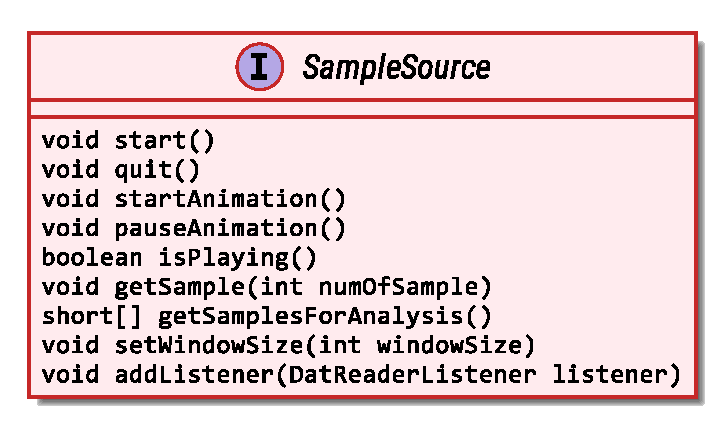
\includegraphics[width=90mm]{figures/ch9/1.eps}
	\caption{Class diagram of the SampleSource interface.}
	\label{fig9.1}
\end{figure}
All its methods are:
\begin{itemize}
	\item start(): it starts the SampleSource and prepare all resources that it needs;
	\item quit(): it stop the SampleSource and destroys all resources used;
	\item startAnimation(): it starts the animation of the ECG signal (scrolling or oscilloscope);
	\item pauseAnimation(): it pauses the animation of the ECG signal;
	\item isPlaying(): it returns true if the animation is active, false otherwise;
	\item getSamples(numOfSamples): it gets from the source numOfSamples samples and stores them;
	\item getSamplesForAnalysis(): it returns D2 lead, used for the ECG analysis;
	\item setWindowSize(windowSize): it sets the size of the display window size, specified in number of samples, that depend on the device screen size and orientation;
	\item addListener(listener): it registers a listener that will be notified if the SampleSource changes animation state.
\end{itemize}
The SampleSource interface that we introduced will be the basis for the following class description, the DatReader, the core of our record ECG opening.

\subsubsection{DatReader}
The DatReader is an abstract class that handles all the most sensitive operations for which regarding ECG record opening. It implements the SampleSource interface, described before, and permits to support many kind of ECG record format, with the only need of overriding one of their methods. There are many things under the hood of this class, so they will be described one by one.\\
The first characteristic of this class is that, all its operation are executed asynchronously from the UI thread: this is done by extending the class HandlerThread, described in the previous chapter. By doing this, we can exploit all the functionalities provided by this class, as the Looper and Message passing mechanism. So the DatReader once started, it will stay watching at its MessageQueue, though its Looper, waiting for a new message. The messages in this class will be basically the number of samples that it will need to read. To read the ECG samples, the DatReader will hold a stream to the record .dat file (file containing all samples). Reading constantly from a file, therefore avoiding the allocation in memory of the record, permits us to maintain the app memory low.\\
But who is sending these messages to the DatReader? Well, there are basically two scenarios:
\begin{itemize}
	\item The user that is using the app scroll the ECG paper with its finger, causing the app to load the right number of samples depending on the movement size and direction;
	\item The user activated the ECG scrolling animation, and so some samples need to be loaded after a certain period, depending on the ECG record rate.
\end{itemize}
Focusing on the first scenario, the entity that will handle ECG visualization and user inputs will be the SampleDisplay, which will be described in details in the next section. And so it will respond to the user scroll, calculating the right number of samples and request them to the DatReader, which is viewed as a SampleSource. The request will be represented by a Message, containing all useful information, like of course the number of samples to load, but also others.\\
There is a problematic where we want to provide scrolling of the ECG paper in both direction, while we are reading constantly from a file: we need to be able to move the file pointer in both direction, not a trivial functionality. The class that we rely on is the RandomAccessFile class: using this class we can always retrieve the actual position of the file pointer and then move it with the method seek(). But this is not the only problematic. We need to take into account that the application will always show on screen a window of the ECG record, with a dynamic size, dependent on the space available on screen. Therefore, the file pointer will refer to a specific point of this window. This point can be the tail or the head of the window, namely the point where the samples were added last time.\\
Consider the following example, represented in the figure \ref{fig9.2}: an user opens a ECG record, the DatReader will be created and started, and will load all the samples need in order to fill the device screen. At this moment, it will have read all the samples sequentially, from the first one to the the last required one, from the file. Thus, the file pointer is referring to the tail of the ECG record window. After that, the user starts scrolling to the right, in order to see the following two seconds of the record. So the DatReader continues to read sequentially the following samples in the file. But now suppose that the user decides to change its scrolling direction and go back. We cannot only read the file backwards from the last pointer position, because those samples will be already loaded and visualized in the sample window. What we need to do is to skip the entire window, and start reading from that point. So after the left scroll, the pointer will be moved to the head of the window.\\
\begin{figure}[ht!]
	\centering
	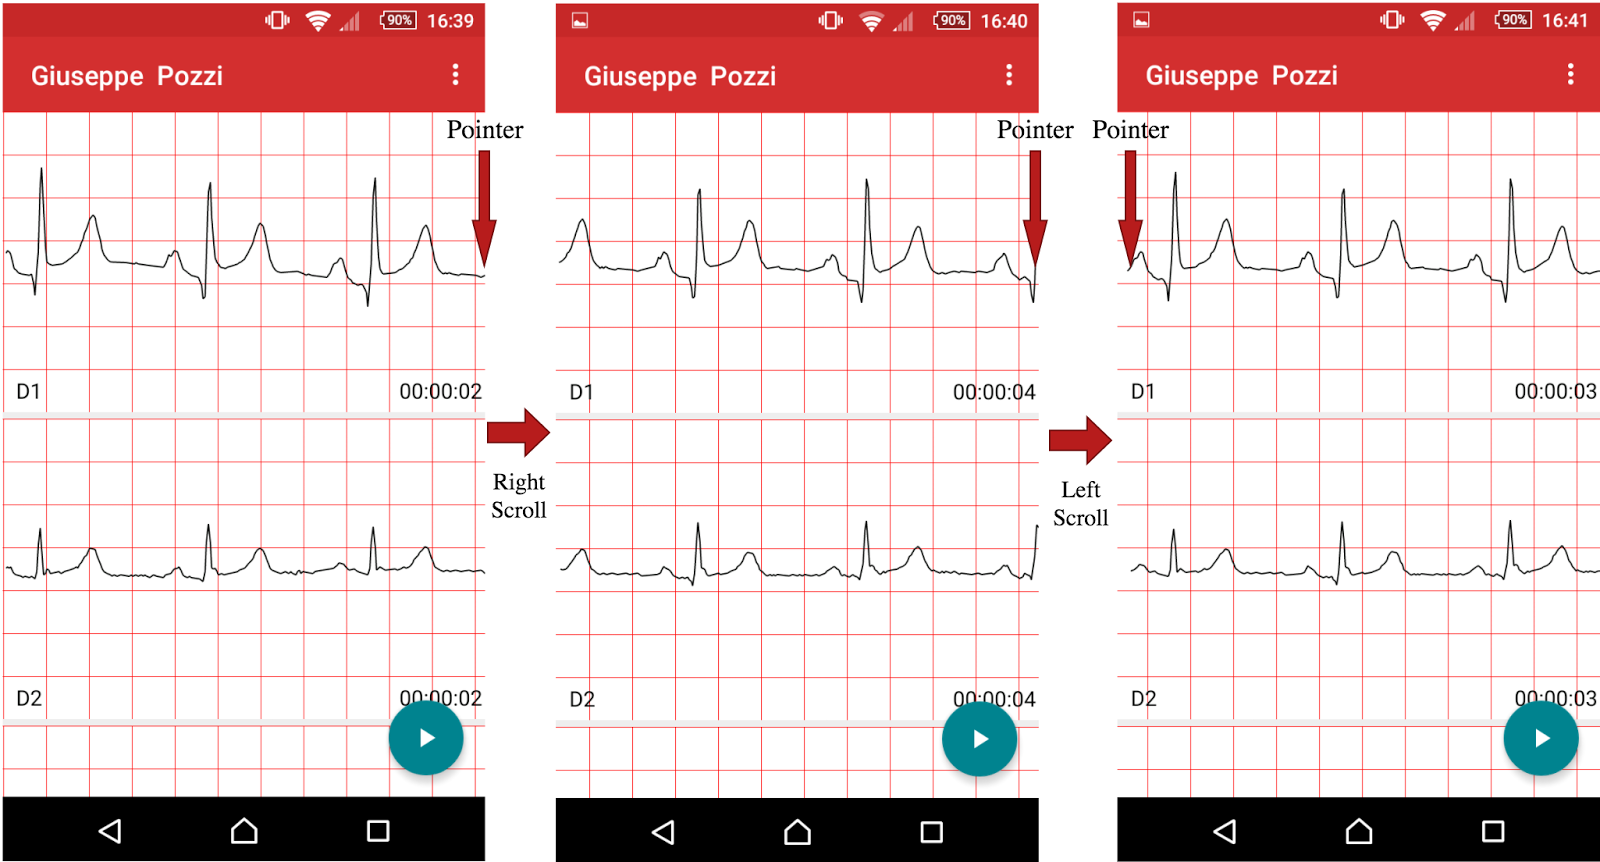
\includegraphics[width=140mm]{figures/ch9/2.png}
	\caption{The movement of the file pointer in the DatReader, after the user change direction of scrolling the ECG paper.}
	\label{fig9.2}
\end{figure}
To make this mechanism possible, it is clear that we have to store the previous reading direction, stored in the variable prevDirection. If the new direction will be different, the DatReader will move the file pointer, skipping the window. So we need also to store the size of the window: this is done with the variable windowSize.\\
After each file reading operation, the DatReader will send to the SampleDisplay all new samples, specifying if add them to the tail of the window or to the head. The iteration between  SampleSource and SampleDisplay in the user scrolling scenario is summarized in the figure \ref{fig9.3}.
\begin{figure}[ht!]
	\centering
	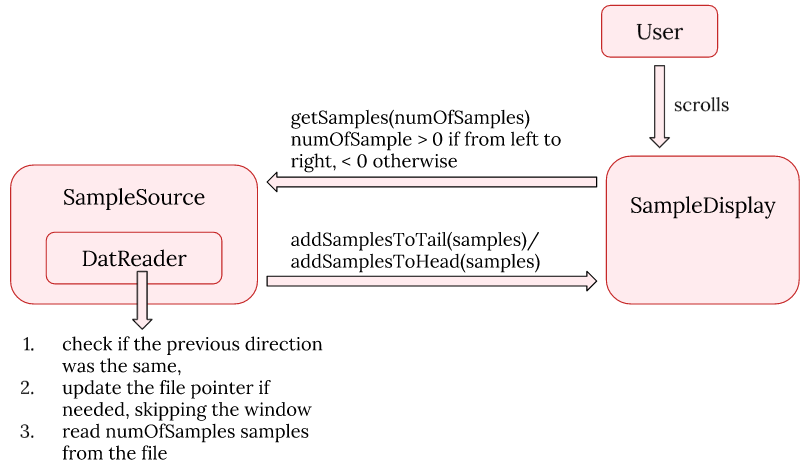
\includegraphics[width=120mm]{figures/ch9/3.png}
	\caption{The iteration between  SampleSource and SampleDisplay after the user scroll the ECG paper.}
	\label{fig9.3}
\end{figure}
Before being sent to the SampleDisplay, the read samples are reconverted to mV, by dividing all values by the gain of the signal. In this way, we can work with universal values during plotting, as different ECG record can have different gain.\\
Now we will move to the second scenario. Here, the user has activated the ECG scrolling animation, by clicking on the play button, which will be binded to the SampleSource, causing the call of startAnimation(). In this case, there will be another entity that will request samples from the SampleSource. The crucial aspect is that, it will continuously requests new samples, but doing so respecting the rate of the original ECG record. This is not a trivial problem, as some requests could be delayed because of another operation that is not finished. So these requests need to be concurrent, reliant on a mechanism to guarantee the right rate, with a good precision. The solution was the adoption of a SheduledThreadPoolExecutor, a pool of thread that we have described in the chapter about concurrency. Thanks to its method:
\begin{lstlisting}
	scheduleAtFixedRate(Runnable command, long initialDelay,
	long period, TimeUnit unit)
\end{lstlisting}
we can program all the requests in the pool by:
\begin{lstlisting}
	scheduledThreadPoolExecutor.scheduleAtFixedRate(new Runnable() {
		@Override
		public void run() {
			getSample(1);
		}
	}, 0, 1000000 / rate, TimeUnit.MICROSECONDS);
\end{lstlisting}
having a precision of microseconds. Being this type of operation not so expensive, we initialized our pool with only one thread.\\
We have omitted that the method getSamples(numOfSamples) doesn’t have an implementation for getting the samples from the source, but it just acts like a request to the SampleSource: by executing it, the implementation in the DatReader will create a message and enqueue it to its MessageQueue. The DatReader will continuously read messages from its MessageQueue and sooner or later, it will find that message, read the sample from the source, and update the SampleDisplay with the new sample. An summarization of the mechanism is showed in the figure \ref{fig9.4}. Furthermore, in the figure \ref{fig9.5}, you can find an overview of the DatReader class, including all variables introduced in this section.
\begin{figure}[ht!]
	\centering
	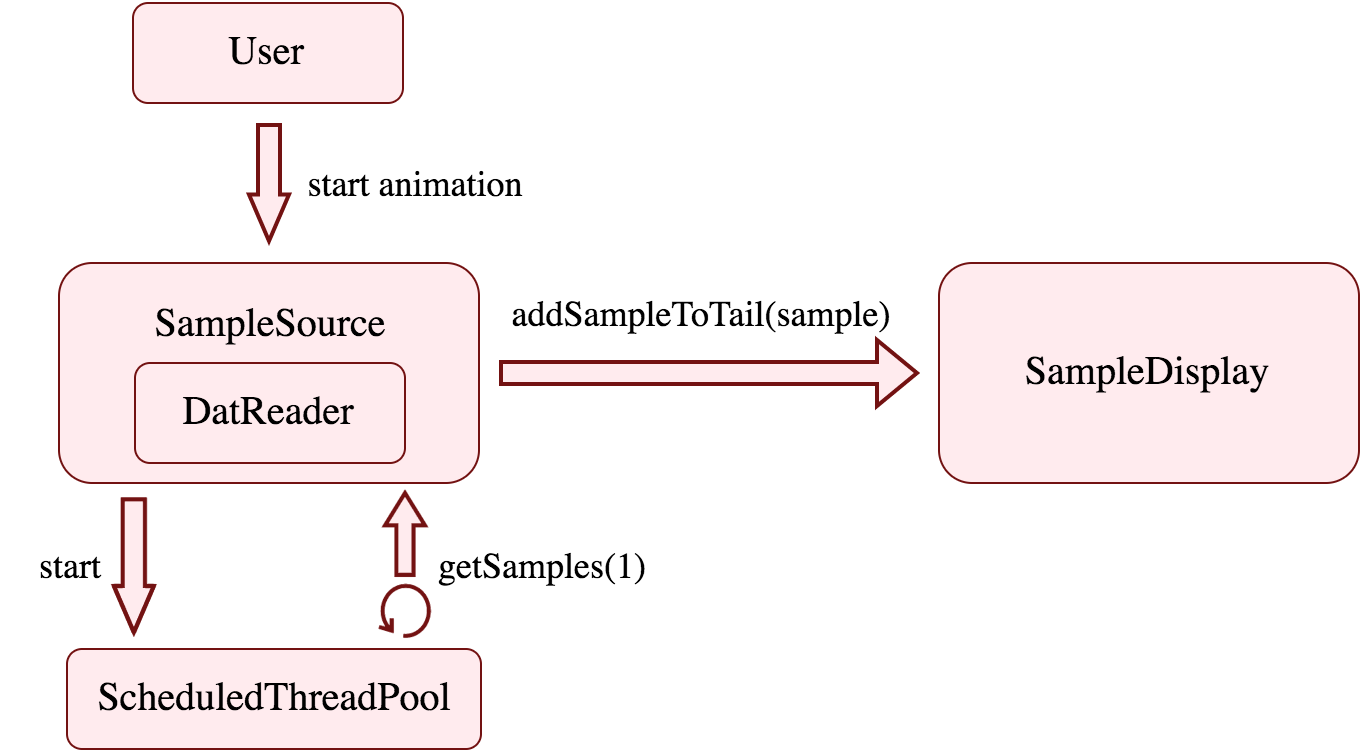
\includegraphics[width=120mm]{figures/ch9/4.png}
	\caption{The animation mechanism of DatReader using SheduledThreadPoolExecutor.}
	\label{fig9.4}
\end{figure}
\begin{figure}[ht!]
	\centering
	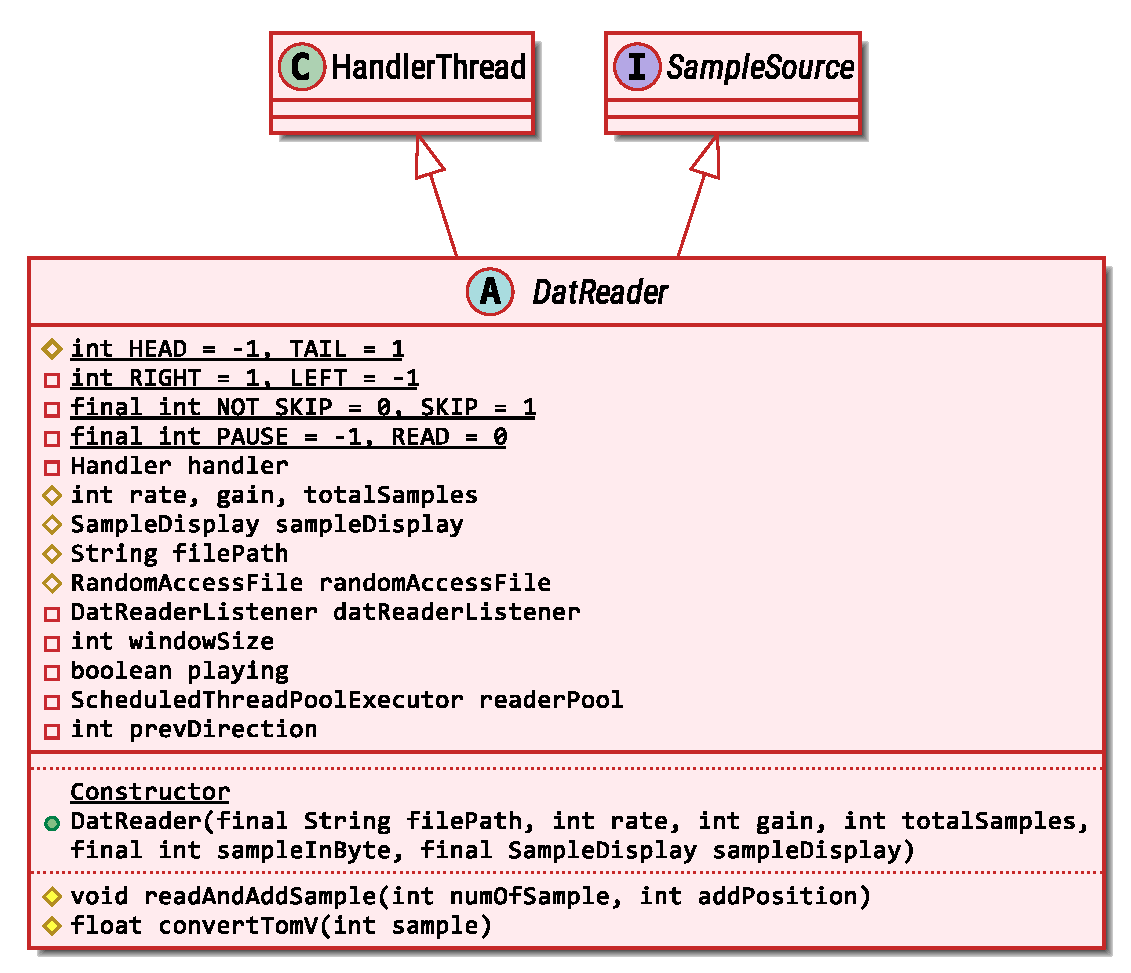
\includegraphics[width=130mm]{figures/ch9/5.eps}
	\caption{Class diagram of the DatReader class.}
	\label{fig9.5}
\end{figure}

\subsubsection{ ZEcgReceiver}
Now we describe the component that will be used during the ECG real-time acquisition. It will communicate with the BluetoothSerial class and interact, similarly to the DatReader, with the SampleDisplay. As the DatReader, it extends the HandlerThread, therefore it will have a personal Looper and MessageQueue. It will also have an acquisitionBuffer that will use to store partial data received from BluetoothSerial. So, what it will do is waiting for new messages on its MessageQueue, and react on a new message. A message coming from BluetoothSerial will contain a buffer of data received from the acquisition device through a bluetooth connection. At a new message receiving , ZEcgReceiver will read the buffer in the message and append it to its acquisitionBuffer. After that,  it will scan its acquisitionBuffer and read all possible samples inside, and free it from all decoded samples. All new decoded samples are then sent to the SampleDisplay for the visualization.\\
ZEcgReceiver will also handle many other operation as:
\begin{itemize}
	\item It will store a heartRateBuffer of the last sample received, with a size of 10 seconds, used to compute the real-time heart rate, to be notified to the SampleDisplay;
	\item It will include the calculation of the Moving Average Filter, if enabled, in order to remove the baseline wander artifact;
	\item The data received from the acquisition device will also include information about its battery level. For this reason, it will parse it and send it to the SampleDisplay;
	\item It will write additional information in the file .hea of the ECG record. 
\end{itemize}

\subsection{Display}
Before we described all the entities behind the generation of the data that will be sent then to the visualization part of the application. Now we will talk about all the components that make ECG visualization possible. Equivalently to the previous section, we will start describing the general interface the will represent the visualization component, the SampleDisplay, moving later to the component that will implement it.

\subsubsection{SampleDisplay}
The have already mentioned many time the SampleDisplay component when talking about data sources. This interface represent the general entity that expose some entry point to add new samples and handle ECG signal visualization. The figure \ref{fig9.6} shows an overview of all methods.
\begin{figure}[ht!]
	\centering
	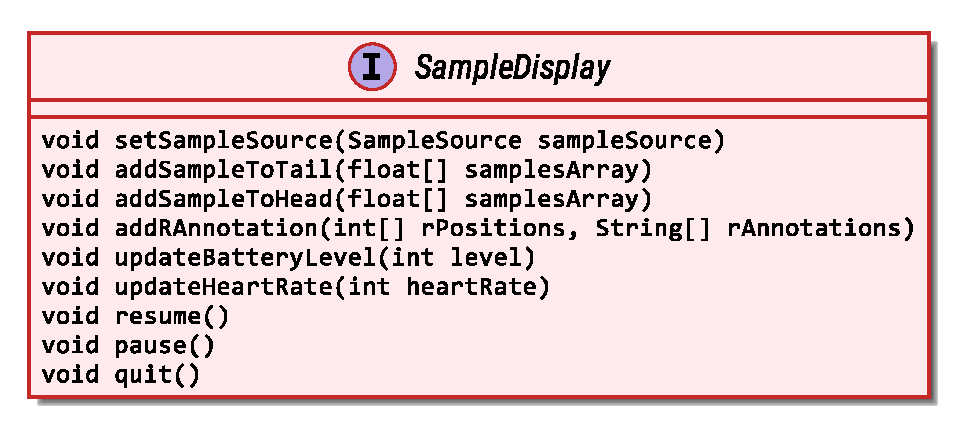
\includegraphics[width=120mm]{figures/ch9/6.eps}
	\caption{Class diagram of the SampleDisplay interface.}
	\label{fig9.6}
\end{figure}
Methods description:
\begin{itemize}
	\item setSampleSource(SampleSource sampleSource): it binds the SampleSource passed as parameter;
	\item addSampleToTail(float[] samplesArray): it adds all samples in the passed array to the tail of the visualized samples window;
	\item addSampleToHead(float[] samplesArray): it adds all samples in the passed array to the head of the visualized samples window;
	\item addRAnnotation(int[] rPositions, String[] rAnnotations): it stores all the R position ( of the QRS complex ), with their relative annotations coming from the ECG signal analysis;
	\item updateBatteryLevel(int level): it updates the visualized battery level;
	\item updateHeartRate(int heartRate): it updates the visualized heart rate in BPM;
	\item resume(): it resumes the ECG signal visualization;
	\item pause(): it pauses the ECG signal visualization;
	\item quit(): it will close and free all the components used for visualization.
\end{itemize}

\subsubsection{SignalScrollView}
For our visualization of the ECG signal we wanted to provide a scrollable view of different ECG paper strip, where in each one was displayed a different ECG lead. Hence, we selected as entity implementing the SampleDisplay interface, a customized version of the ScrollView class, a scrollable view provided in Android. This class will be the entry point for all data sources, and a container for some other components, described in details further on. These contained elements will be the all SignalSurfaceViews, where each one represent the view of an ECG lead. The SignalScrollView represents also the core for one of the feature described in the previous chapters: the dynamic display scaling. It will do all calculation inside its method calculateMetrics(). The goal of the method is calculate the size of the basic block of the standard ECG paper, which is 0.5 cm, in pixel. The problem is that the pixel size varies a lot, being dependent on the device screen pixel density. So for doing this, we need to retrieve the pixel density of the device screen, and then calculate properly the right size of the blockInPixel( figure \ref{fig9.7} ). 
\begin{figure}[ht!]
	\centering
	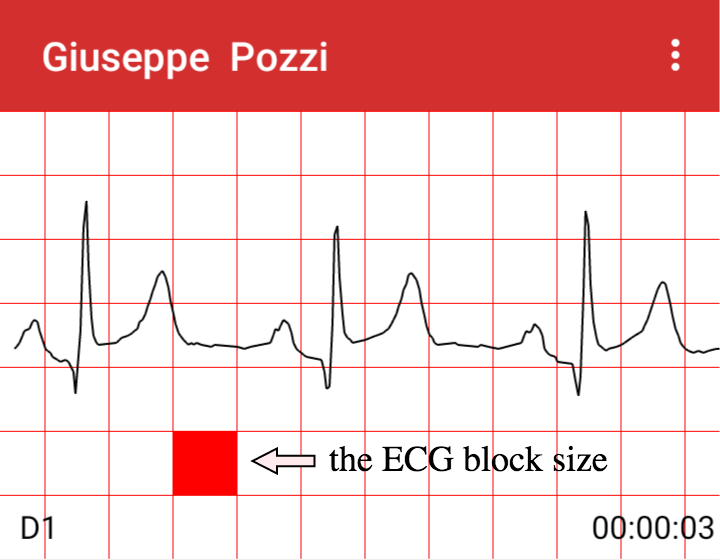
\includegraphics[width=90mm]{figures/ch9/7.png}
	\caption{The size of the ECG paper block after the computation of the method calculateMetrics().}
	\label{fig9.7}
\end{figure}
The measure used to represent the pixel density is the \textit{dpi (dots per inch)}, defined as \textit{“the number of individual dots that can be placed in a line within the span of 1 inch (2.54 cm)”}.\cite{ref24} The formula for the computation of the blockInPixel will be:
\begin{equation}
	blockInPixel=\frac{dpi*blockInCm}{inchInCm}
\end{equation}
where:
\begin{itemize}
	\item \textit{dpi}: screen pixel density, dependant on the device specification;
	\item \textit{blockInCm}: the size of the ECG paper block in centimeters, equals to 0.5 cm;
	\item \textit{inchInCm}: the size of one inch in centimeters, equals to 2.54 cm.
\end{itemize}
With this calculation we can ensure a perfect scaling in many device, with a very small error percentage for high pixel density screens ( $\sim$240dpi or higher ).\\
The method calculateMetrics() take place in the initialization process of the class, together with the method fillScrollView(int heightInBlock). This method receives the parameter heightInBlock, which comes from the app settings and specifies the height of the ECG paper strip in ECG standard blocks, and create and add inside the SignalScrollView all the SignalSurfaceViews needed, depending on the number of ECG signal leads (one per lead). Moreover, during its initialization, the class will create another important component, the DrawingHelper, that we will describe next. This last will handle all the call of the SampleDisplay methods:
\begin{itemize}
	\item addSampleToTail(float[] samplesArray);
	\item addSampleToHead(float[] samplesArray).
\end{itemize}
For this reason, SignalScrollView will route each adding request to the DrawingHelper, that will take care of storing the visualize samples window and adding all new samples to it.\\
Furthermore, SignalScrollView will perform a very important optimization for the visualization of the ECG paper strip: with its method pauseNotVisibleView() will be able to select only the strips that are present in the screen, and pause the drawing routine ( described in the next sections ) for all not visible strips, saving lot of computational power. This method will be triggered every time the user will scroll the view.\\
Lastly, we need to specify that SignalScrollView will also handle drag events coming from the user when he wants to scroll the ECg paper. But the class will be used as reference class both during real-time acquisition and ECG record opening. The difference in these scenario is that, during real-time acquisition, the dragging need to be disabled, while in the other, enabled. So to achieve this distinction, inside the constructor will be passed the parameter dragEnabled, which will be used to activate or not the overridden method onTouchEvent(MotionEvent ev), that will take care about decode the performed scroll and notify the SampleSource.\\
	As usual, an overview of the class could be seen in the figure \ref{fig9.8}.
\begin{figure}[ht!]
	\centering
	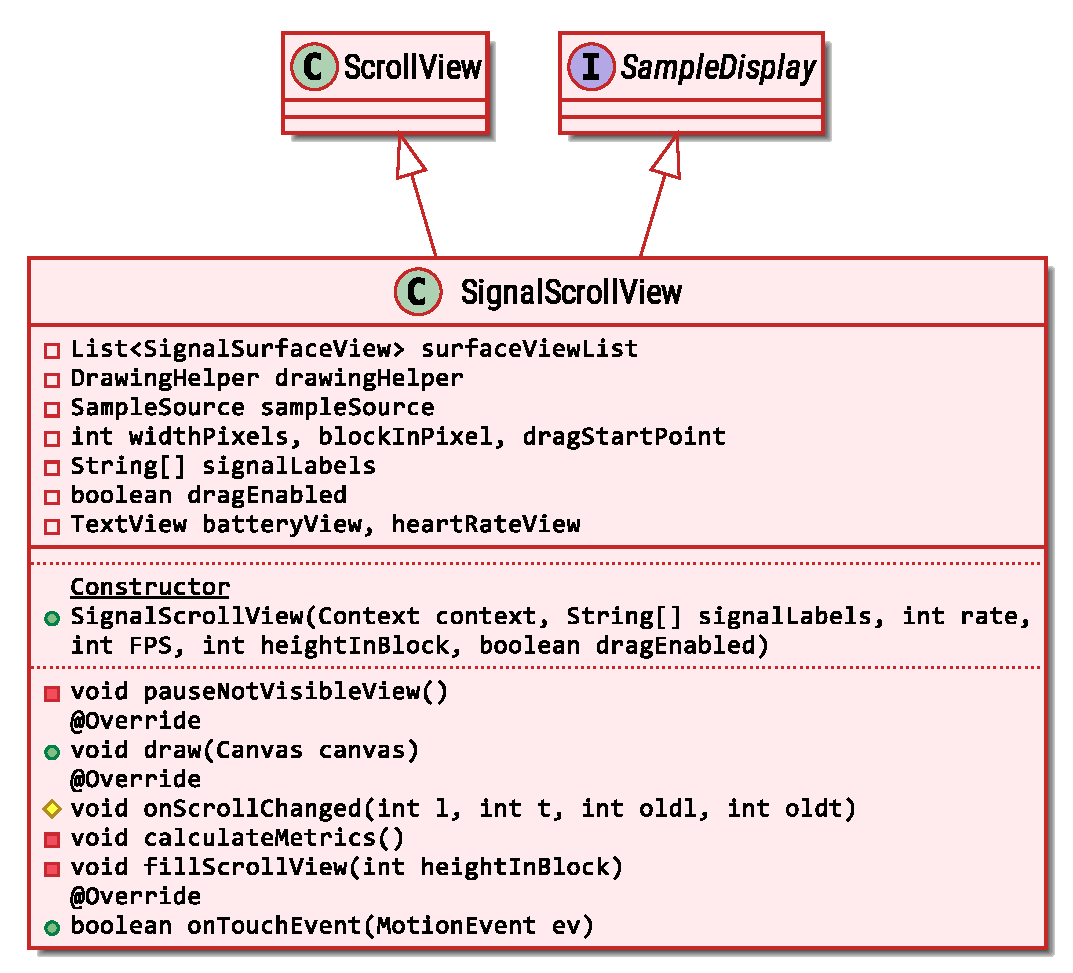
\includegraphics[width=130mm]{figures/ch9/8.eps}
	\caption{Class diagram of the SignalScrollView class.}
	\label{fig9.8}
\end{figure}

\subsubsection{SignalSurfaceView}
In  order to achieve the best performance, we used the best mechanism available in Android for fast and custom drawing. For this purpose we extended the class SurfaceView. As explained in the Android developer site \textit{“The SurfaceView is a special subclass of View that offers a dedicated drawing surface within the View hierarchy. The aim is to offer this drawing surface to an application's secondary thread, so that the application isn't required to wait until the system's View hierarchy is ready to draw. Instead, a secondary thread that has reference to a SurfaceView can draw to its own Canvas at its own pace.”}\cite{ref25}. We will focus on the thread responsible of drawing on the SignalSurfaceView when will describe the Drawer class. For now, we describe only the main operation of the SignalSurfaceView. This class will be liable of reacting after the creation of the view and on view change event. This last will occur typically after a rotation of the device screen, performed by the user. This will cause for example to change the orientation from portrait to landscape, and so the new SignalSurfaceView will be required to fill all the new available space.

\subsubsection{DrawingHelper}
As the name suggests, this is the helper class for all drawing operation. Many of its methods and variables will be used by the Drawer for handle drawing. It is an abstract class, because we provide to different plotting type: a scrollable drawing and a oscilloscope drawing ( figure \ref{fig9.9}). For each type, there is a proper extending  class:
\begin{itemize}
	\item DrawingHelperScroll, for scrollable drawing type;
	\item DrawingHelperOsc, for oscilloscope drawing type.
\end{itemize}
\begin{figure}[ht!]
	\centering
	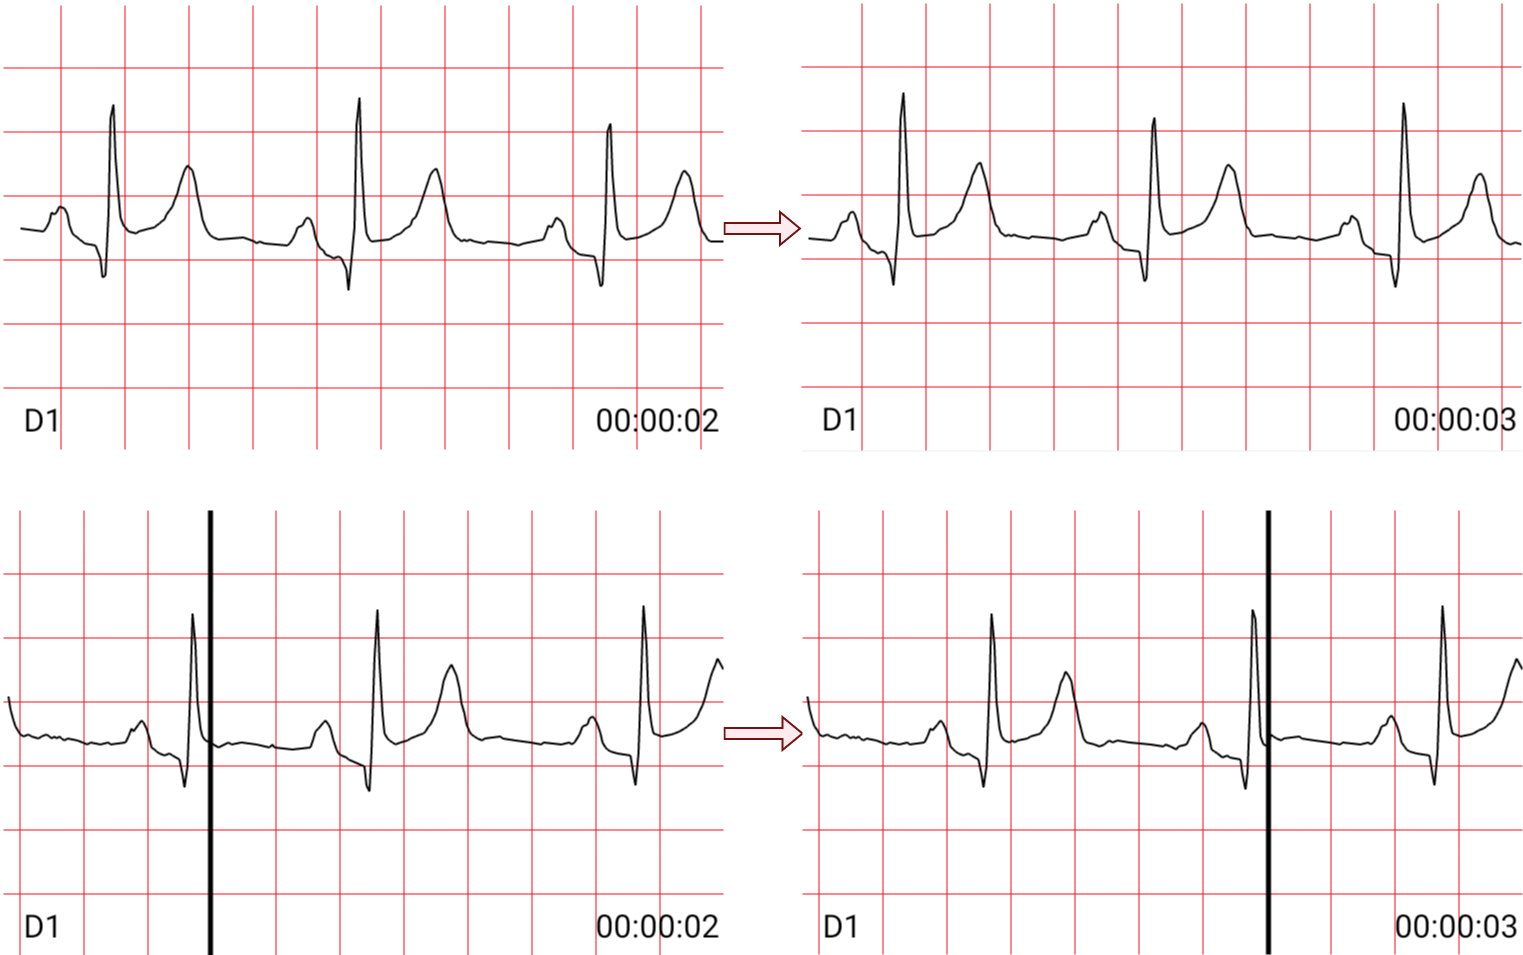
\includegraphics[width=100mm]{figures/ch9/9.png}
	\caption{The different ECG visualization types. The one on top is the scrolling drawing, the one in the bottom is the oscilloscope drawing. The time elapsed after the movement of the ECG paper is one second.}
	\label{fig9.9}
\end{figure}
Each of these class will store the list of all sampleWindows, containing a sampleWindow for each ECG lead. The sampleWindow will store the samples window that is currently visualized on the screen. The collection type for the sampleWindow is different in the two classes, because each one use the most suitable implementation for its update type. For example, the DrawingHelperScroll, will treat the window as a queue: it will always add new sample to the head or to the tail. Thus, it uses a ArrayDeque, an very efficient and fast class when applied to this type of scenario.\\
During its initialization, with the method prepare(args ...) the DrawingHelper creates some Drawer. This last is the class used for drawing on the SignalSurfaceView, and will be described in the next section. The number of Drawer created depends on the computational power availability of the device used: in the method the DrawingHelper will retrieve the number of cores available in the device CPU, and will create accordingly the same number of  Drawer ( which, you will see, will extend the HandlerThread class ). For this reason, with a single core CPU, only a Drawer will be created, and it will be the sole handler for all the SignalSurfaceView ( and so all ECG strips ). Instead, if we had four CPU core, and for example all the twelve ECG leads, there will be created four Drawer, where each will handle the drawing of three SignalSurfaceView. This characteristic provide a nice performance scalability, dependent on the CPU of the used device.\\
The DrawingHelper also will handle the lifecycle of all Drawers using:
\begin{itemize}
	\item startDrawing(int signalIndex), for starting the drawing operation of the Drawer which is the handler for the passed signalIndex;
	\item pauseDrawing(int signalIndex), for pausing the drawing operation of the Drawer which is the handler for the passed signalIndex;
	\item quit(), for stopping all Drawers currently active and destroying them.
\end{itemize}
Furthermore, the DrawingHelper will provide the helper methods, used by the Drawer, to compute the different drawing layers:
\begin{itemize}
	\item drawGrid(Canvas c, Paint p): it draws the ECG grid in the passend Canvas using the passed Paint. It uses the variable blockInPixel for the right sizing;
	\item drawSignalLabelsAndTime(int signalIndex, Canvas c, Paint p): it draws the labels of the time and the ECG leads in the passend Canvas using the passed Paint;
	\item drawSamples(int signalIndex, Canvas c, Paint p): it draws all the samples inside the sampleWindow as lines in the passend Canvas using the passed Paint. It avoid the drawing of consecutive equals value when plotting the lines, in order to save useless operations;
	\item drawRAnnotations(Canvas c, Paint p): it highlights all the R peaks by drawing vertical lines on them and with the respective R annotation, in the passend Canvas using the passed Paint. This of course will be active only after the analysis.
\end{itemize}
In the figure \ref{fig9.10} you can find the class diagram of the DrawingHelper class.
\begin{figure}[ht!]
	\centering
	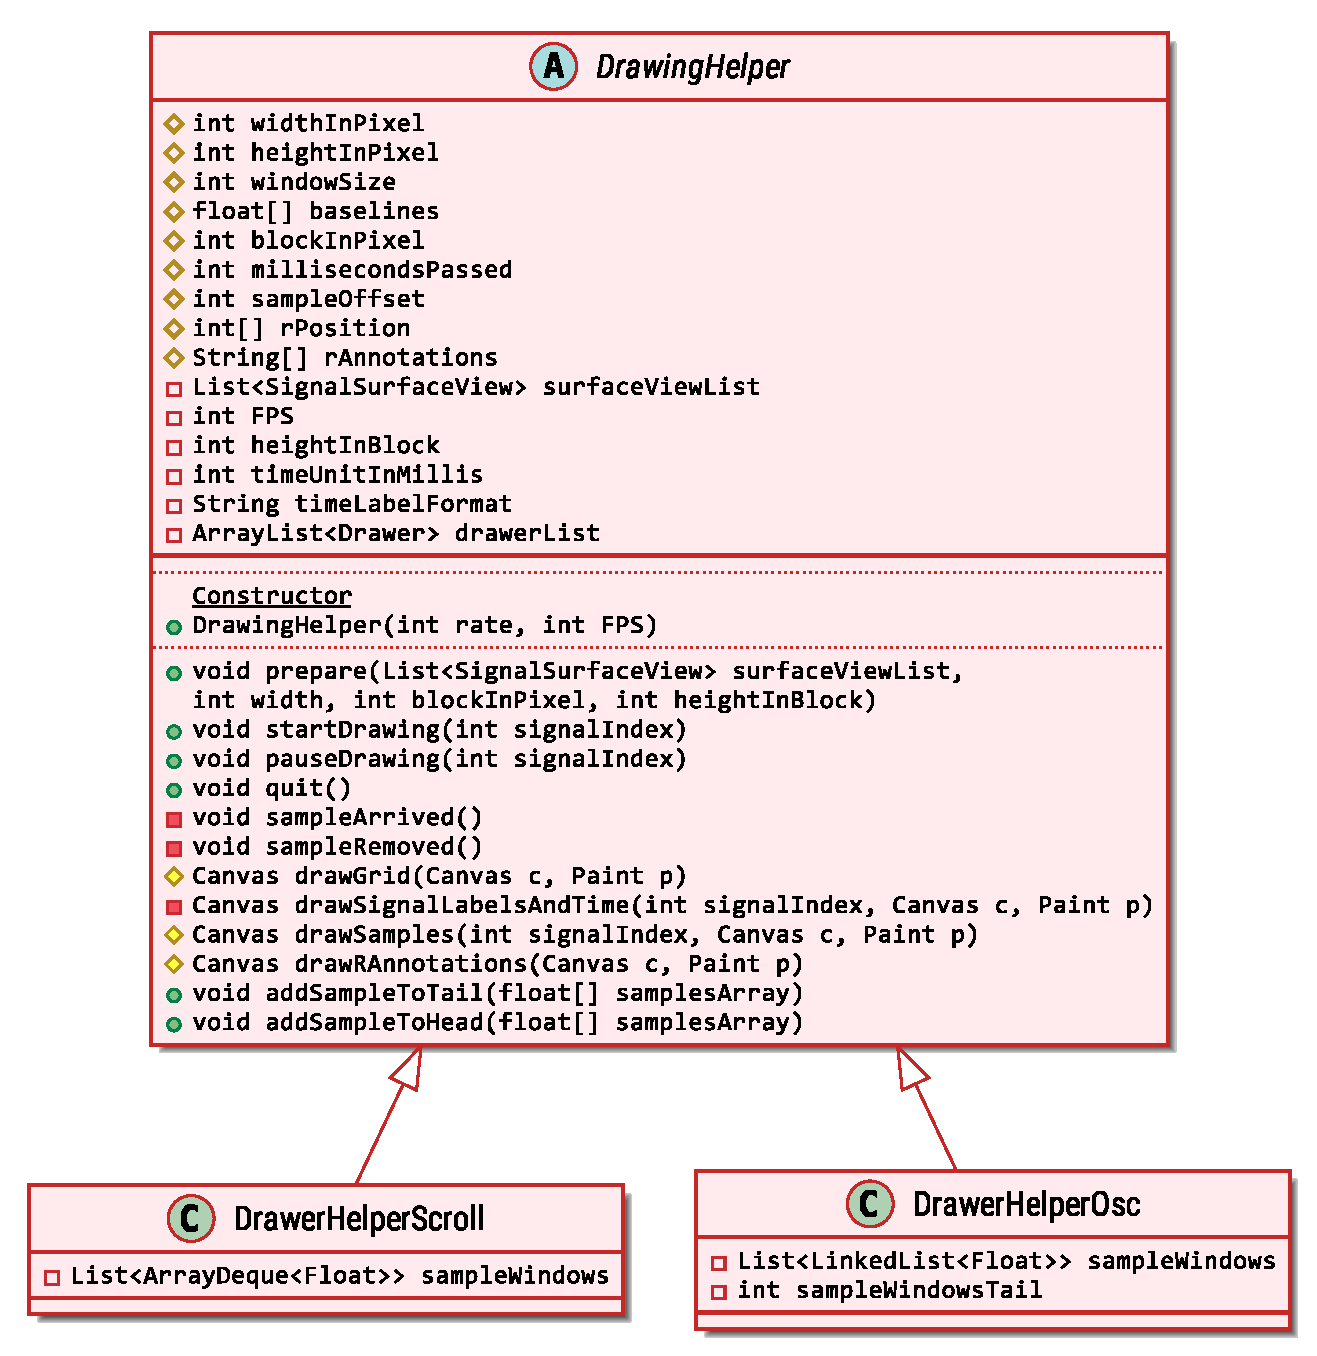
\includegraphics[width=140mm]{figures/ch9/10.eps}
	\caption{Class diagram of the DrawingHelper class.}
	\label{fig9.10}
\end{figure}

\subsubsection{Drawer}
As already mentioned earlier, the Drawer class will be a thread, responsable of drawing on one or more SignalSurfaceViews. It is a private static inner class of the DrawingHelper, and it hold a WeakReference to the DrawingHelper in order to avoid as much as possible memory leaks.\cite{ref26} It extends the HandlerThread class and its basic functioning is reading and responding to all messages sent to its MessageQueue. The messages will contain the index of the ECG lead that need to be drawn. Actually, there will be always only one message per ECG lead on its MessageQueue: this is because, beside of the lead index, all messages are equals, and incorporate the same drawing routine including all drawing method seen in the previous section. But each message at the end will also include a recursive sending of the next message to the MessageQueue, delayed by the time unit dictated from the specified FPS of the application. So each message will cause a sending of the next message. In this way, the Drawer we can continuously draw and update the SignalSurfaceView, at a rate of FPS. The starting of drawing will be managed by the DrawingHelper, which will send the first recursive message. The pausing, manage by the same, will be easily achieved by the removal of all the messages present in the MessageQueue at that moment.\\
In the figure \ref{fig9.11} is showed the class diagram of the Drawer.
\begin{figure}[ht!]
	\centering
	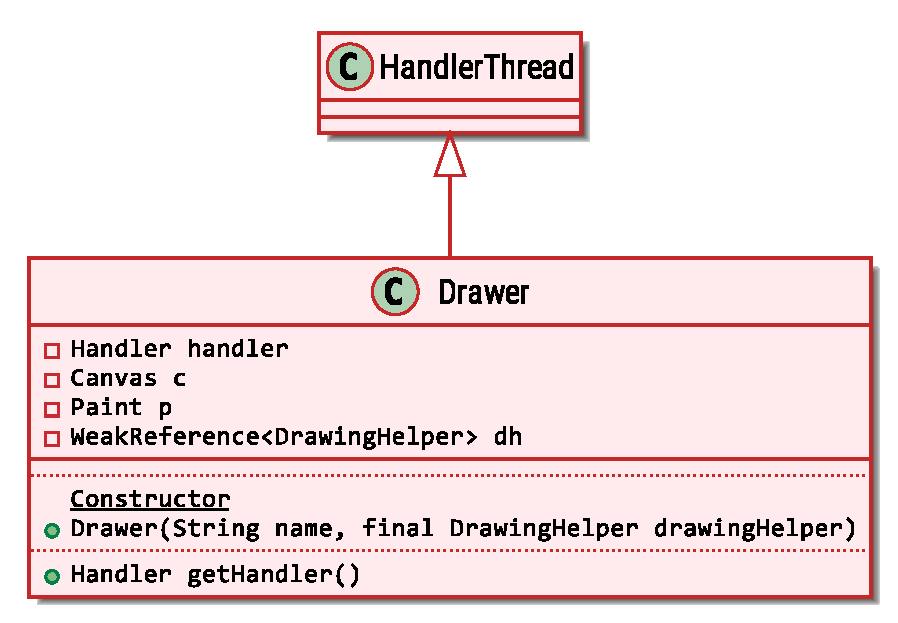
\includegraphics[width=100mm]{figures/ch9/11.eps}
	\caption{Class diagram of the Drawer class.}
	\label{fig9.11}
\end{figure}

\subsection{Connection}
As we have often mentioned, the communication between the acquisition device and the app will rely on a bluetooth connection. There are mainly two different situation where we are using this type of connection:
\begin{itemize}
	\item During the device connection menu, where we use bluetooth to scan all nearby devices in order to find ZEcg;
	\item During real-time acquisition, when we are connect to the device and start receiving the patient ECG samples.
\end{itemize}
In the first case, we made use of a BroadcastReceiver, which will be notified during bluetooth scanning, when a new device will be found. As we don’t want to include external devices in the device scan list, we filtered all devices by name, and included only devices with a name containing the word \textit{“ecg”}.\\
In the second case we made use of the class BluetoothSerial, which is an external library that we have modified and included in our application. The type of connection between two devices differs according to the specific bluetooth modules mount on the different devices we tested our application with. For most of the devices we could establish an unsecure connection with Zecg, without any  security protocols nor explicit  pairing request. On other devices the connection was established only after an explicit pairing request. Either way the Zecg was always the server side and the smartphone the client side of the Bluetooth connection. Whenever a client closes the connection with the server, the connection is automatically lost and any other device can ask data from the server.

\subsubsection{BluetoothSerial}
As we have said when we were talking about the ZEcgReceiver, the BluetoothSerial class will pass data received from the acquisition device to the last by sending messages to it. This is done by using an Handler instance that is passed in the BluetoothSerial constructor, that is pointing to the MessageQueue of the ZEcgReceiver. The messages will include the partial data received from the bluetooth connection, that will be parsed as we described in the ZEcgReceiver section. BluetoothSerial will create different thread, where each one will handle a different connection step:
\begin{itemize}
	\item AcceptThread: this thread runs while listening for incoming connections. It behaves like a server-side client. It runs until a connection is accepted (not used in our case, as the smartphone always act like a client in the connection);
	\item ConnectThread: this thread runs while attempting to make an outgoing connection with a device. It runs straight through. The connection either succeeds or fails;
	\item ConnectedThread: this thread runs during a connection with a remote device. It handles all incoming and outgoing transmissions (only incoming in our case).
\end{itemize}
In the ConnectedThread the message sending will take place.

\subsection{Operations Flow}
In the previous sections we went deep to some component implementations in order to clarify some of the main functioning and iterations. Therefore, we move from a low level description, to an higher level, in order to explain the flow of the app operations. We will focus on our main two operation flow:
\begin{itemize}
	\item Record acquisition: the user acquires a new ECG record by connecting to the acquisition device;
	\item Saved record opening: the user open a stored ECG record, choosing one of them from a list, and visualizes it.
\end{itemize}
For the sake of clarity, we put aside technical terminology for activity describing, as some methods call may be not so explanatory for the understanding. Instead, we used a general description of each activity, being all the details in the previous sections.

\subsubsection{Record acquisition}
\begin{figure}[ht!]
	\centering
	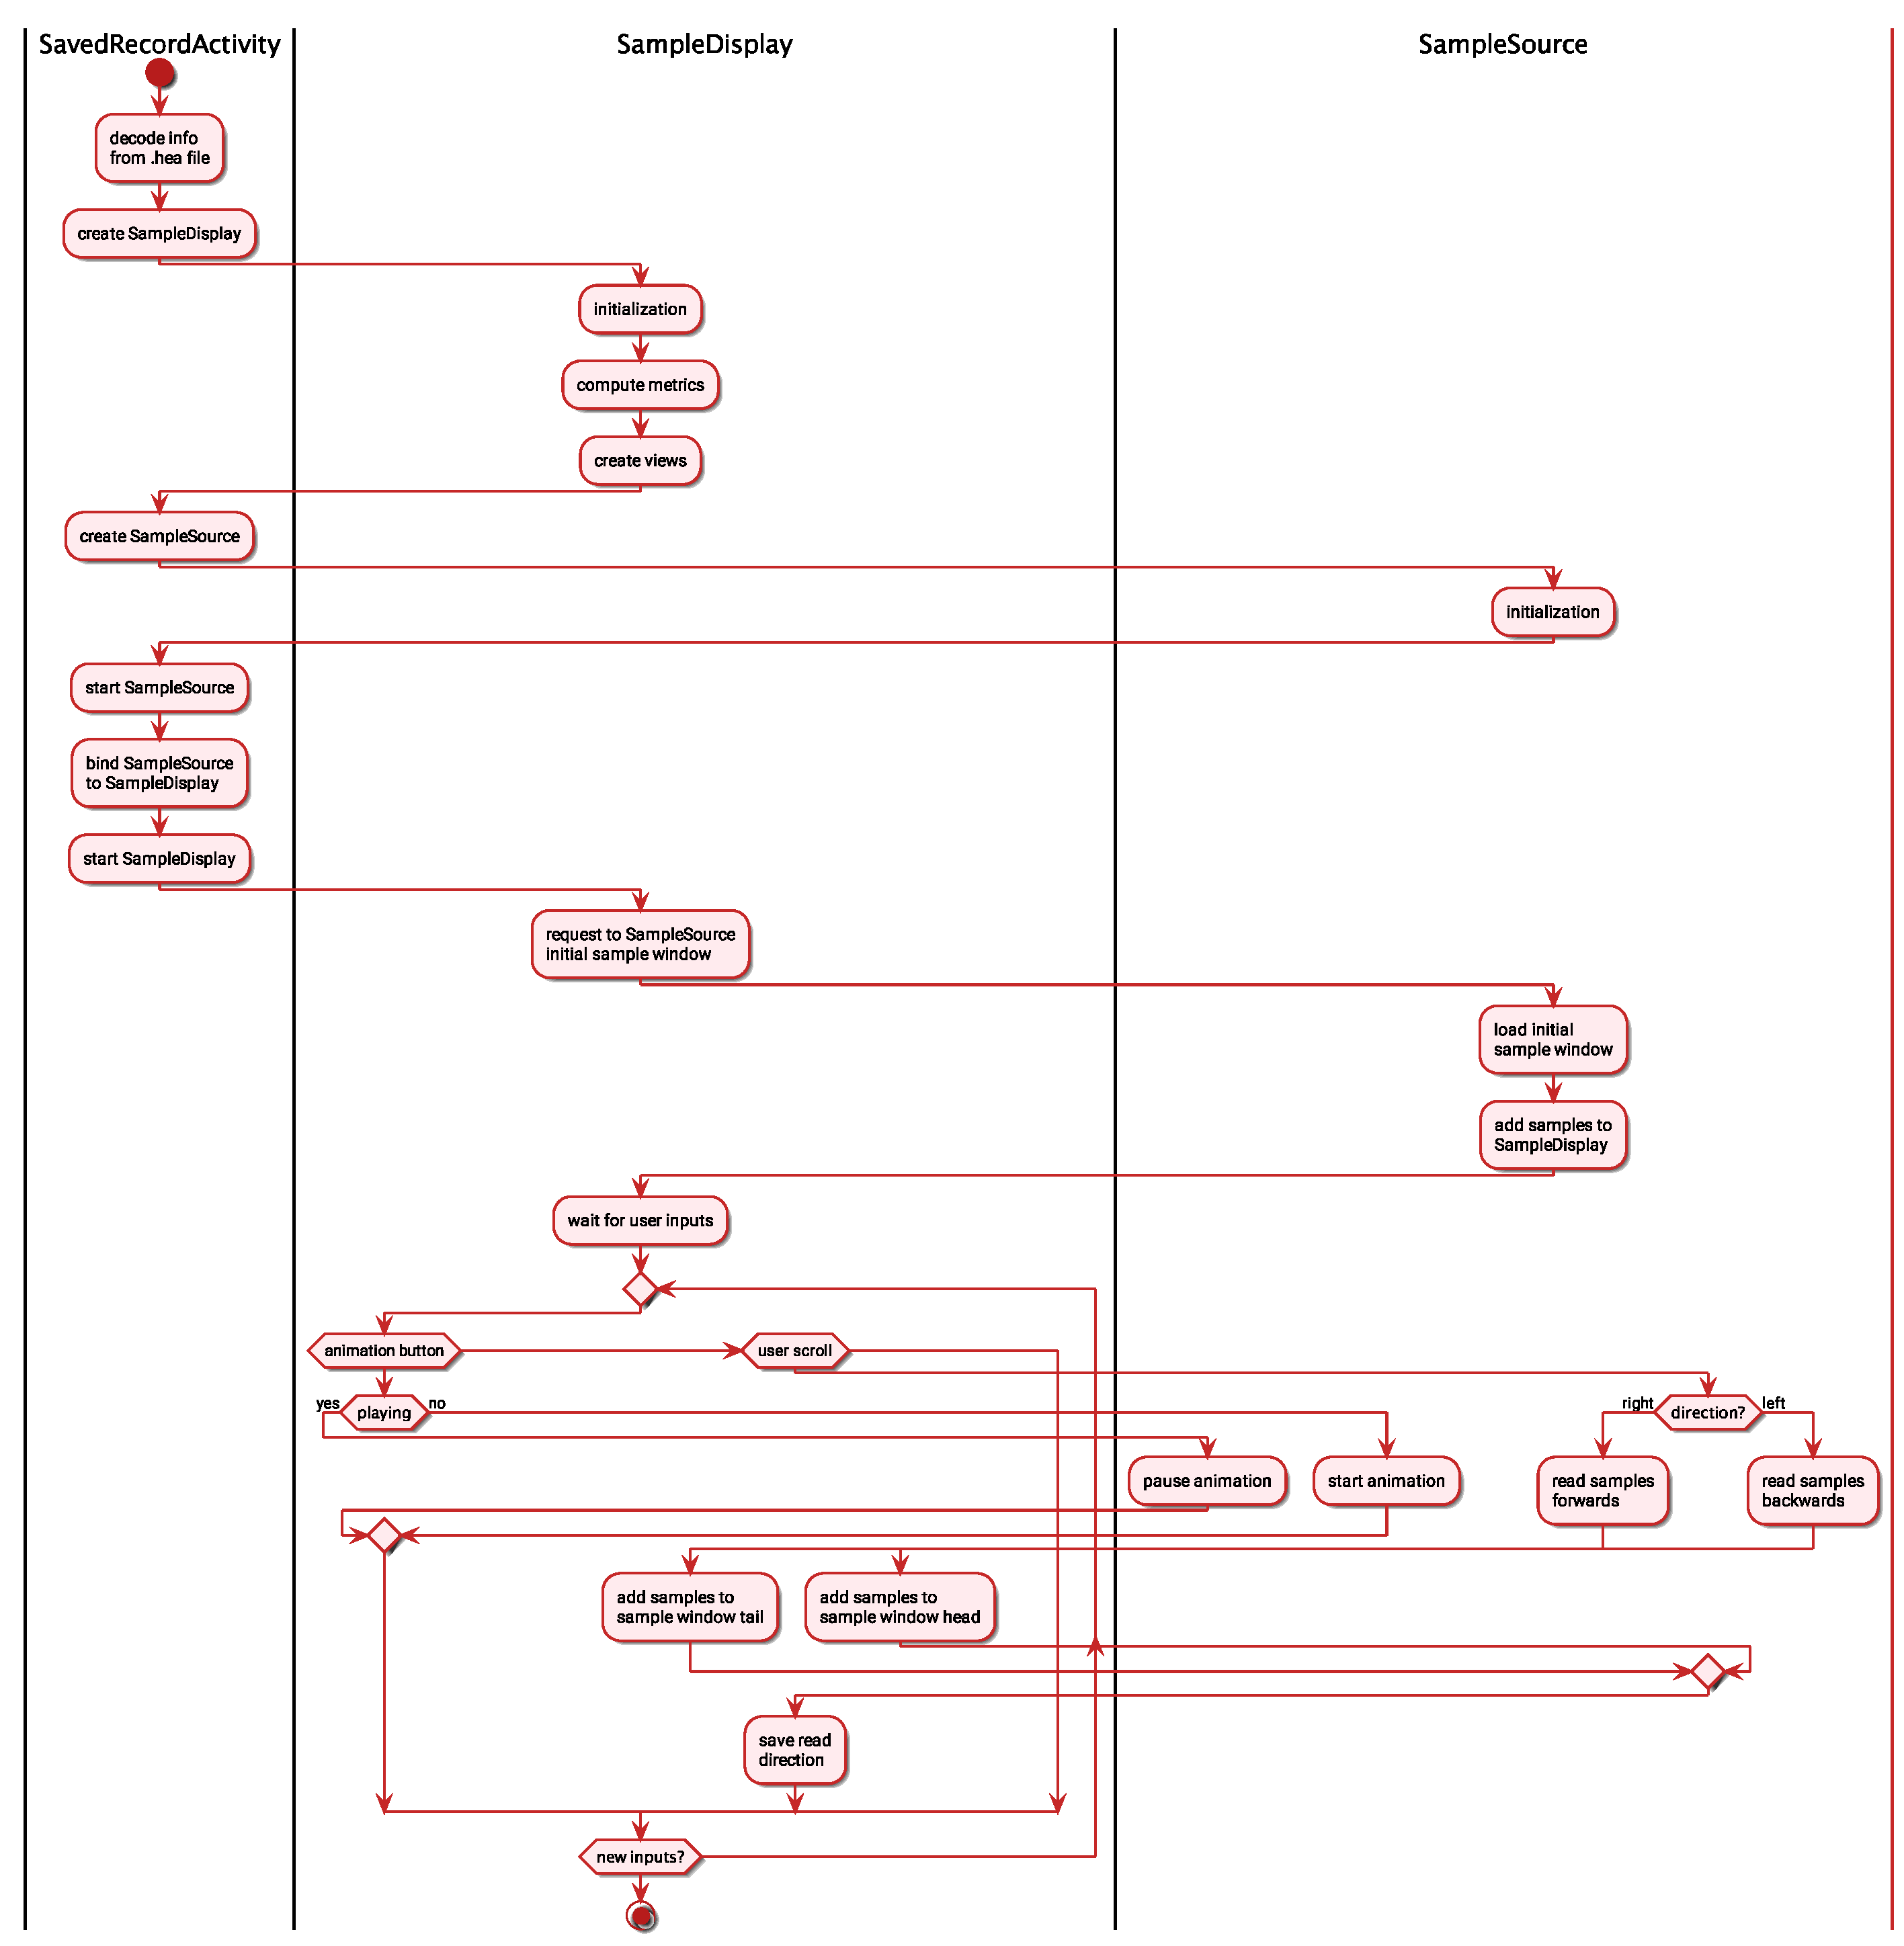
\includegraphics[width=\linewidth]{figures/ch9/12.eps}
	\caption{Activity diagram of a new ECG record acquisition operation.}
	\label{fig9.12}
\end{figure}
The process starts with the selection of \textit{“New Record”} in the app home. After that the user will move to the CreateNewRecordActivity, where will be displayed a form where the user will be required to specify his:
\begin{itemize}
	\item Name,
	\item Surname,
	\item Sex,
	\item Age,
	\item Weight.
\end{itemize}
If the user will omit some information, and clicks on the submit button, an error will be displayed, asking the user to complete the form. After a positive check of the form, there will be the creation of the .hea, including all the previous user data, and the .dat file, the container of all ECG record samples.\\
Then, the bluetooth connection of the device will be checked: if deactivated, the user will be jumped to the DeviceConnectionActivity, where will be able to activate it and search for the acquisition device; if activated, the BluetoothSerial will start the connection with the device, and wait for the first data. At each new data arrival, it will send a message with the new data to the ZEcgReceiver class. This last after having received the message, will extract the new data and insert it into a acquisition buffer. Then it will try to empty the buffer, removing all complete samples. All removed sample will be decoded and added to the sample window tail of the SampleDisplay.
The process of acquiring new data and pass it to the ZEcgReceiver continues until the user will click on the stop button. Afterwords, the connection will be close and additional data will be written to the .hea record file. The operations flow are depicted as an activity diagram in the figure \ref{fig9.12}.

\subsubsection{Saved record opening}
\begin{figure}[ht!]
	\centering
	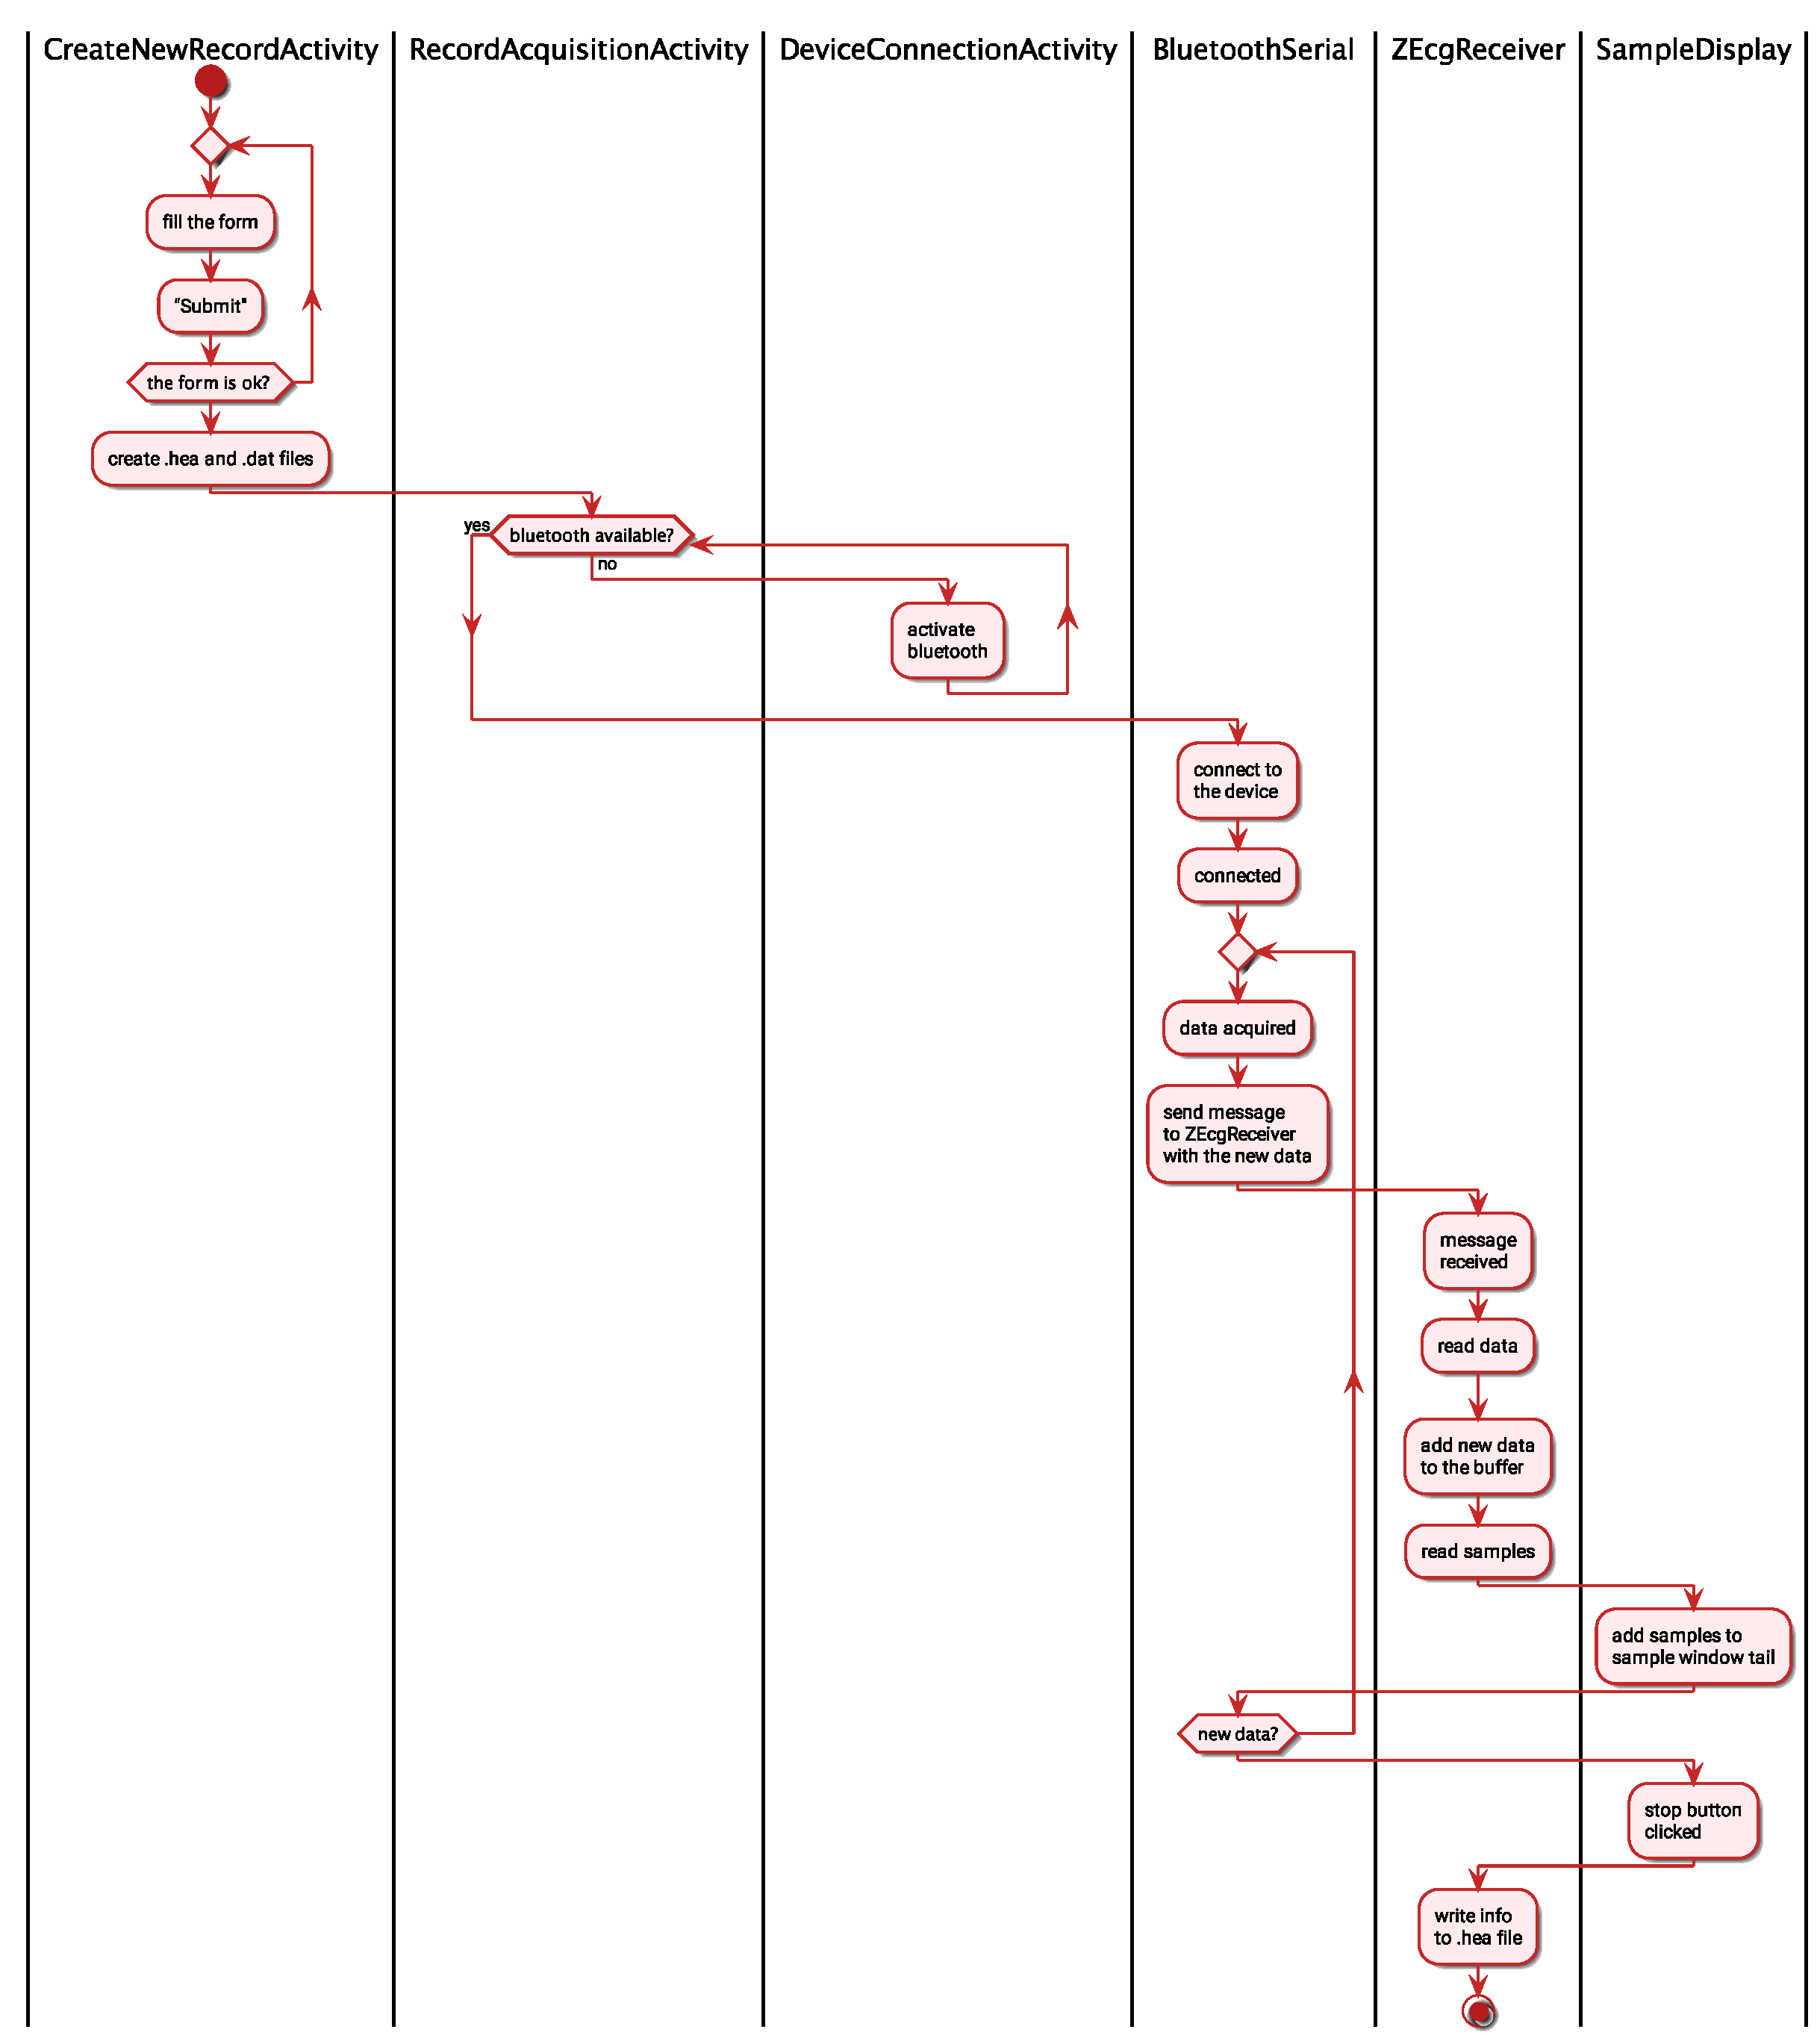
\includegraphics[width=\linewidth]{figures/ch9/13.eps}
	\caption{Activity diagram of a new ECG record acquisition operation.}
	\label{fig9.13}
\end{figure}
The process starts with the selection of \textit{“Open Record”} in the app home. A list of all stored ECG record will be presented to the user. The user will be able to scroll the list and select a ECG record to open it. After that it will be moved to the SavedRecordActivity, where the record .hea file will be decoded to extract all useful information, as sample rate, number of lead, lead labels, signal gain and others. Then, the SampleDisplay component will be created: this will compute all the metrics for which regarding the dynamic ECG paper sizing, and will create all ECG paper strip views. Subsequently, the SampleSource will be created and initialized and binded to the SampleDisplay, which will be started. At start, the SampleDisplay will request from the SampleSource the initial sample window, in order to fill the ECG lead strips created previously. Later, the SampleDisplay will start waiting for any user input. The user input will be of two types:
\begin{itemize}
	\item Animation button click;
	\item Scrolling.
\end{itemize}
In the first case, the state of the animation will be queried:
\begin{itemize}
	\item If playing, the animation will be stopped;
	\item Otherwise, the animation will be started.
\end{itemize}
In the second case, according to the scrolling direction, the respective samples will be read and added to sample window tail or head, respectively if right or left.\\
The process of processing new user inputs continues until the user will close the record visualization. The operations flow are depicted as an activity diagram in the figure \ref{fig9.13}.
%Chapter 10
\chapter{Final result}
ECG-ira (ECG instant rapid analyzer) is a fully working mobile software application able to replace and fulfill most of the functionalities of an analog desktop application. The solution was designed according to the best mobile application development principles and it resulted working fine on all the smartphones\footnote{Samsung Galaxy SIII Mini, Samsung Galaxy Note N7000, OnePlus X, Sony Xperia Z3 Compact, Sony Tablet Z, Huawei P8 Lite} we tested it on. In this chapter we will show the final results providing significant screenshots of the application and metrics related to the performances evaluated and calculated with the application running on different devices.
\section{App Screens}
By launching the application the first screen is the home screen. It is the starting point, here the user can create a new record (starting a new acquisition with the ZEcg device), he can open the list of records (previously acquired or already present in the device system folder), he can discover and establish  a connection with an acquisition device for future acquisitions and he can access to the application settings section where he can customize the application behaviour and tune some settings like the default folder to store in and open the records from.
\begin{figure}[!htb]
\centering
\subfloat[The home screen of the application ECG-ira.]{	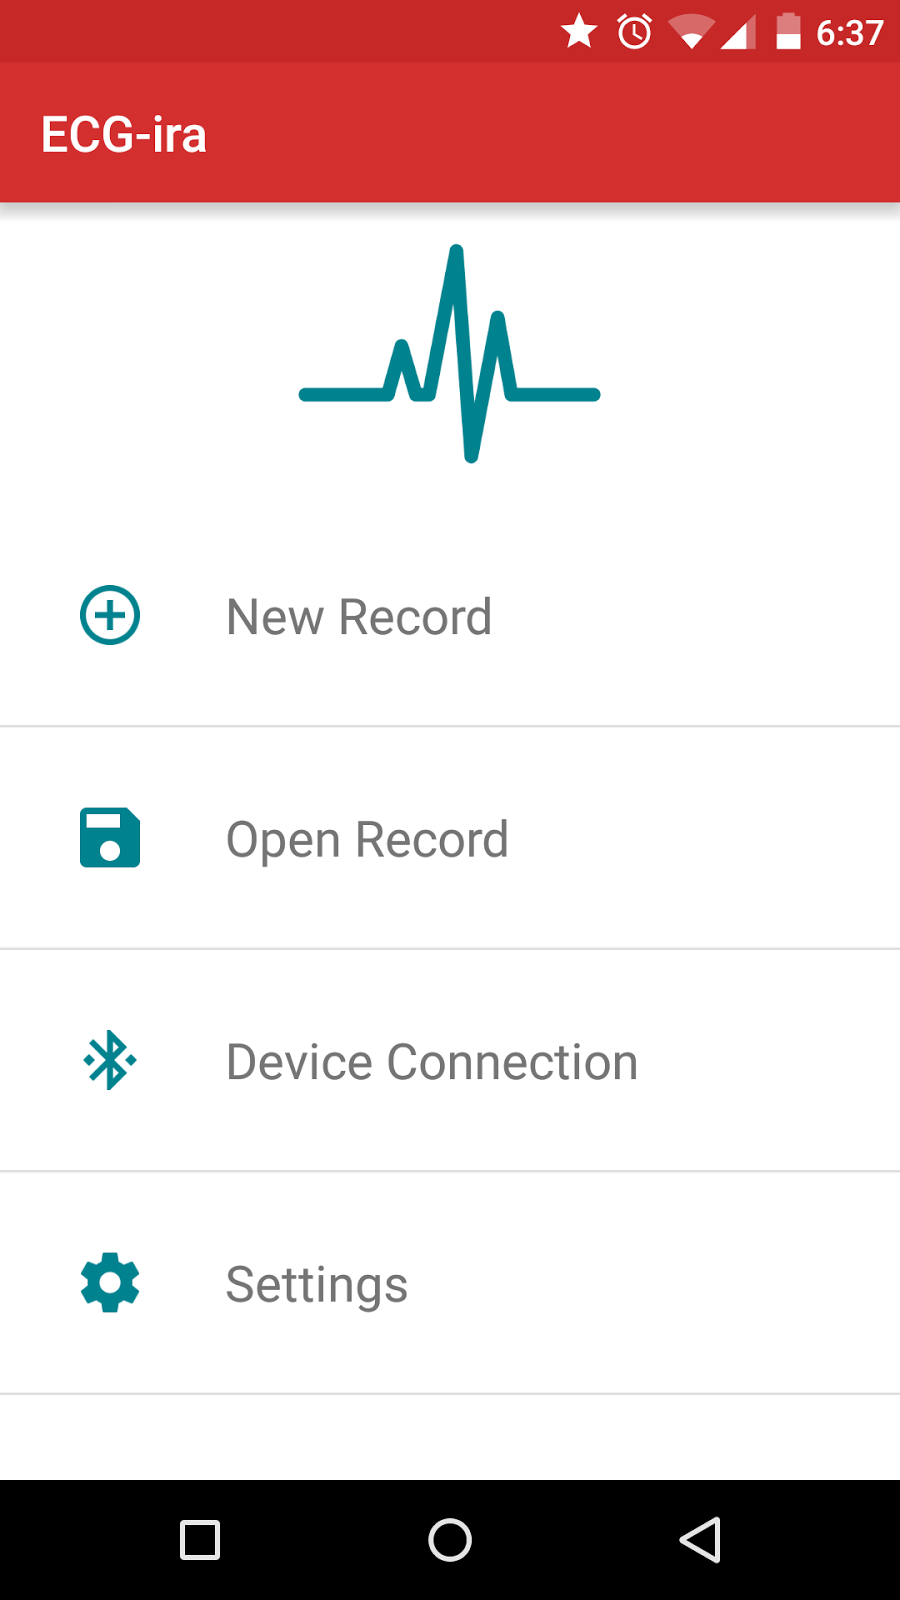
\includegraphics[width=0.3\linewidth]{figures/ch10/1.png}\label{fig10.1}}
\qquad
\subfloat[The form to be compiled before a record can start. It is necessary to bind any record to a patient data in order to avoid confusion between ecg records. This data is also useful for a fully understanding of the record itself]{	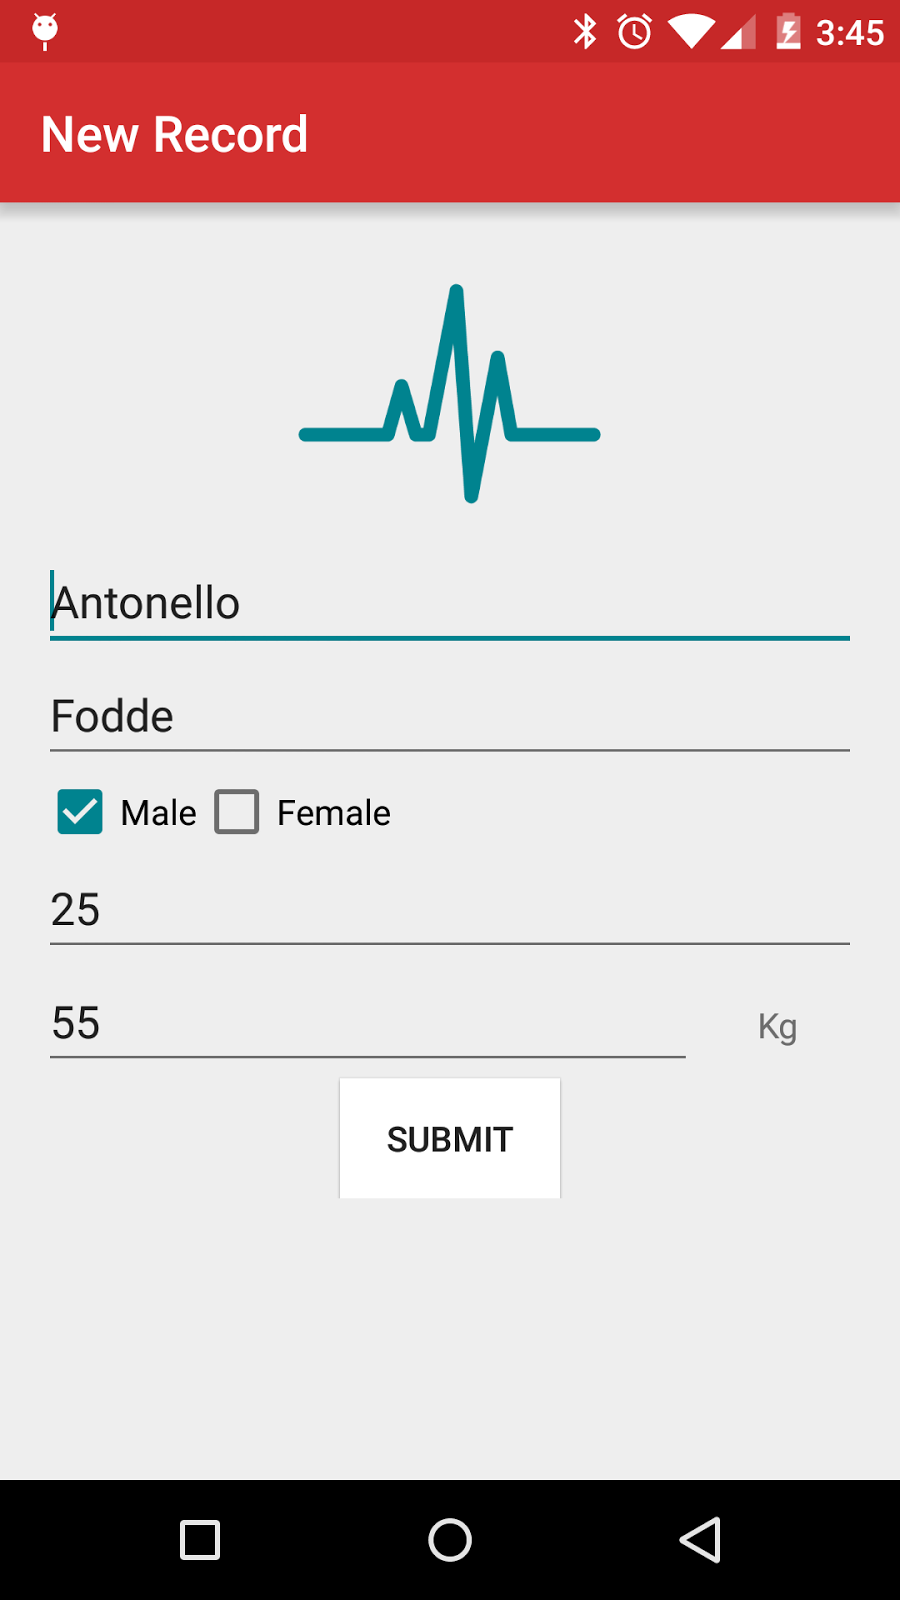
\includegraphics[width=0.3\linewidth]{figures/ch10/2.png}\label{fig10.2}}
\caption{Two screens of the application, respectively the home screen and the form screen to be compiled by the patient}  
\label{fig10.1ab}
\end{figure}
\\By clicking on the “New Record” button option (see figure \ref{fig10.1}), the user will be asked to fill a form with his data as a patient. This data will be then stored within a header file (with .hea extension)  together with the file containing the effective record (.dat file extension). The personal data are only used by the doctor to identify the patient records.\\
Over the submission of the form the file .hea is immediately created to store all the information. If the device is already connected with an acquisition device ZEcg, the application tries immediately to establish a connection to receive data and visualize it (see the acquisition screen in the figure \ref{fig10.3}). Otherwise it opens a connection request activity to enable the Bluetooth and start to discover nearby Bluetooth devices.\\
\begin{figure}[!htb]
	\centering
	\subfloat[A real time ECG acquisition from the Zecg acquisition device.]{	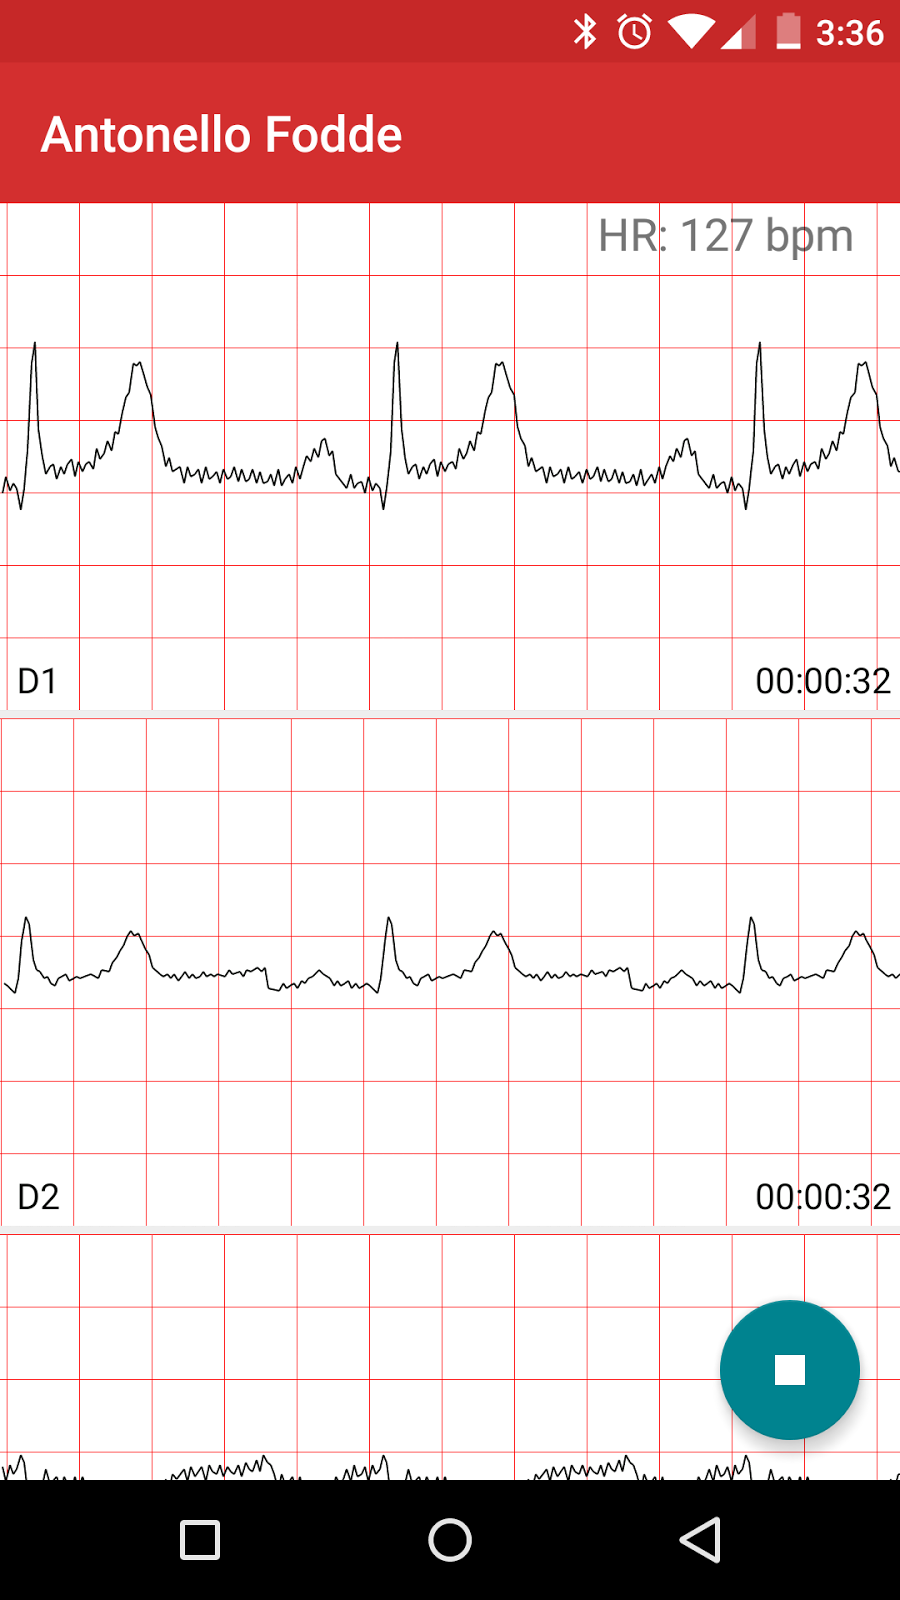
\includegraphics[width=0.3\linewidth]{figures/ch10/3.png}\label{fig10.3}}
	\qquad
	\subfloat[List of records within the device default  folder]{	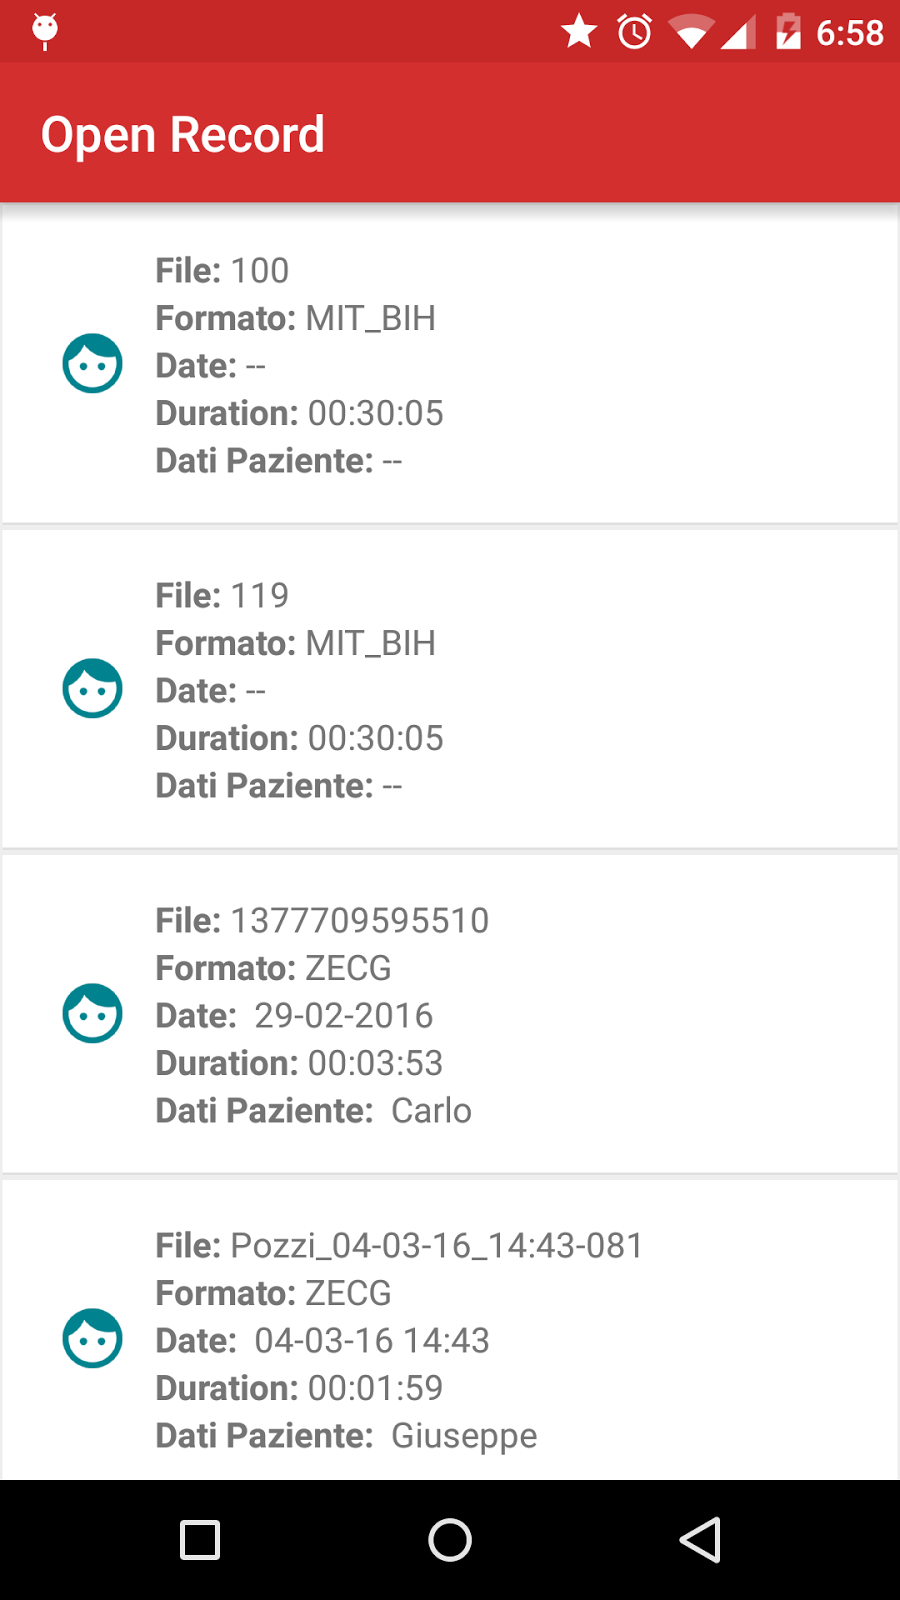
\includegraphics[width=0.3\linewidth]{figures/ch10/4.png}\label{fig10.4}}
	\caption{Two screens of the application representing the realtime acquisition and the list of records within the device}  
	\label{fig10.3ab}
\end{figure}
Going back to the home screen (figure \ref{fig10.1}), by clicking on the “Open record” option button the user will access a list of ECG records saved (figure \ref{fig10.4}) on its own device on a predefined root folder within the device system memory (the default folder can be changed within the setting section).\\
For each record the most relevant information are highlighted:
\begin{itemize}
	\item File Name
	\item File Format
	\item Acquisition Date
	\item Duration in time of the record
	\item Name of the patient
\end{itemize}	
For more details about each record it is possible to long press on the desired record to show up a ToolBar shown in figure \ref{fig10.5}.\\
\begin{figure}[!htb]
	\centering
	\subfloat[Screen triggered by long pressing on a list item. At the bottom of the screen there is a ToolBar showing the info and the delete options described above.]{	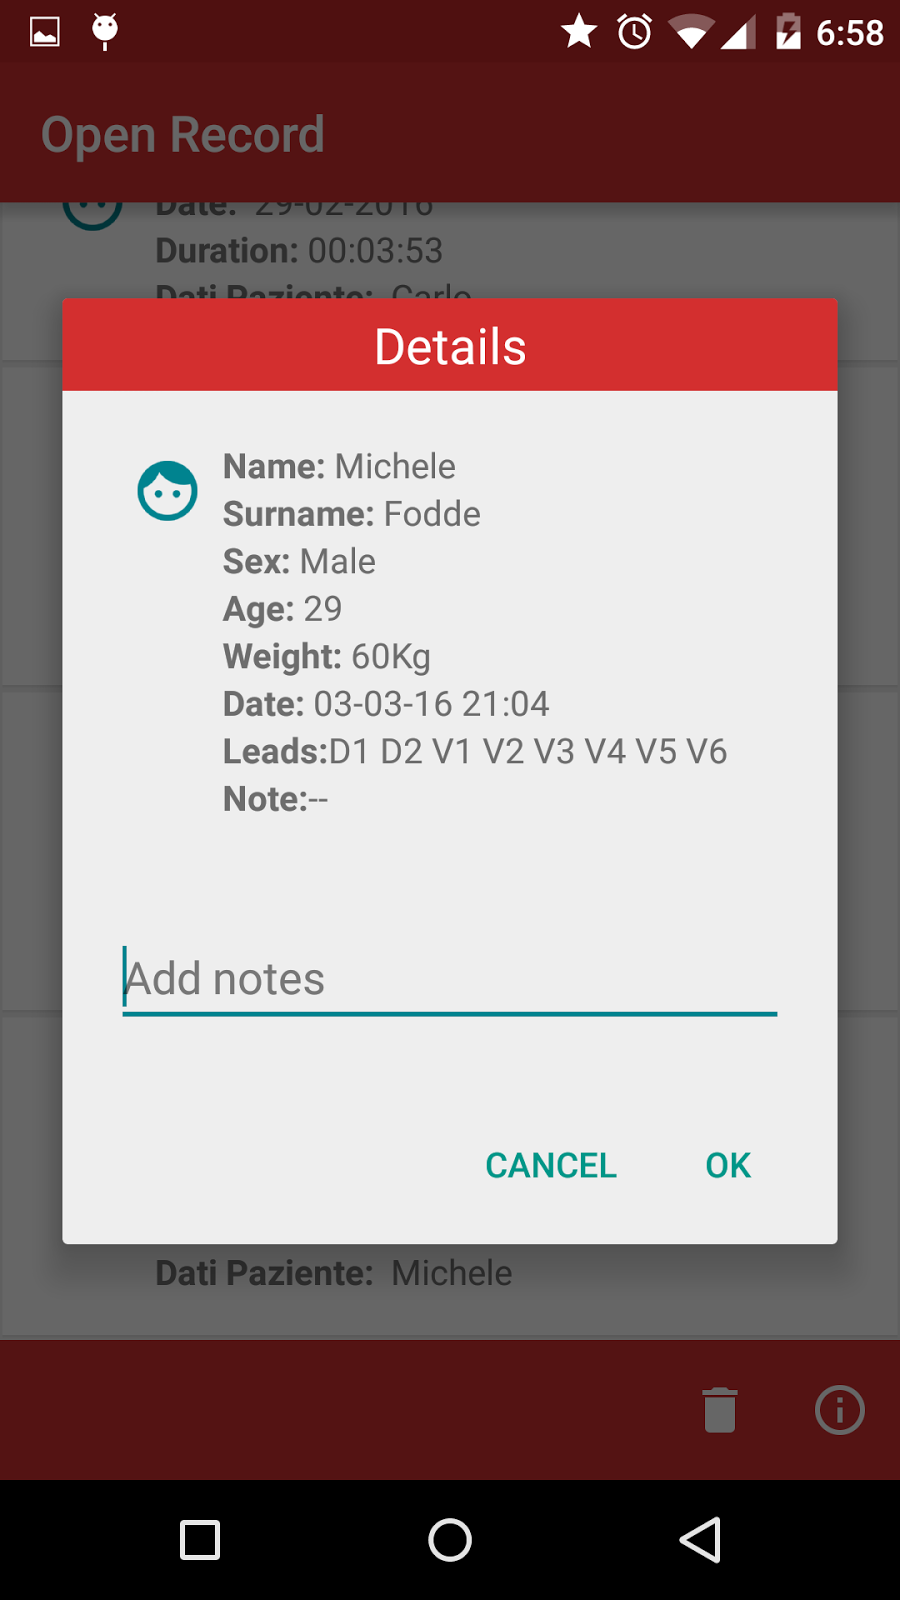
\includegraphics[width=0.3\linewidth]{figures/ch10/5.png}\label{fig10.5}}
	\qquad 
	\subfloat[An example of record opening and plotting. In the screen a MIT-BIH record format was opened.]{	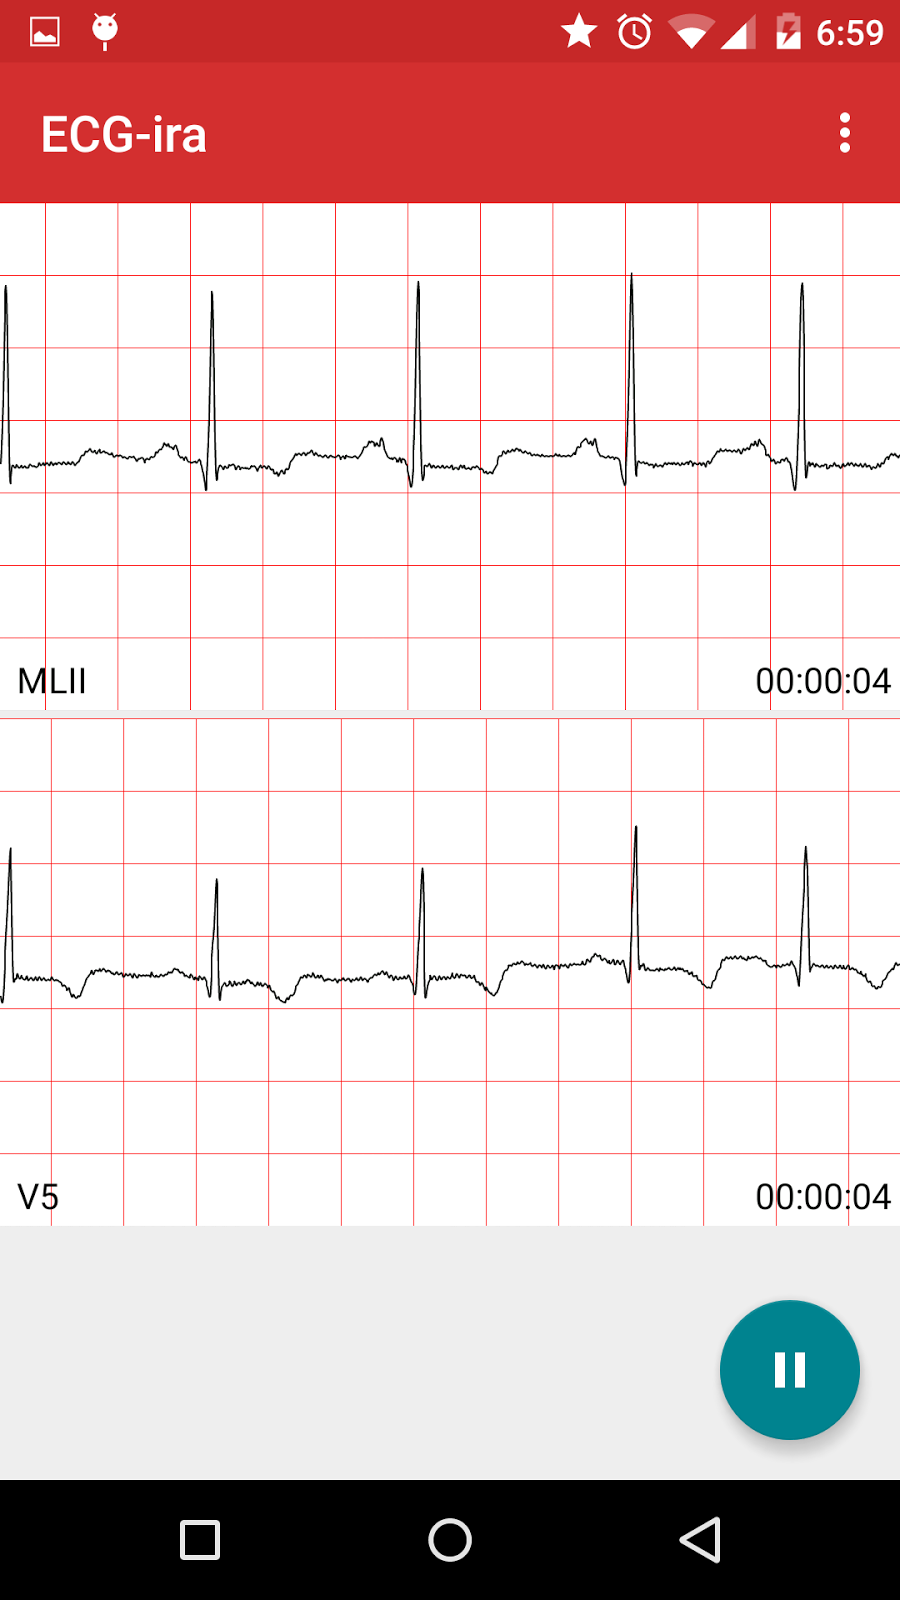
\includegraphics[width=0.3\linewidth]{figures/ch10/6.png}\label{fig10.6}}
	\caption{Two screens of the application representing the info dialog for a certain record and the visualization of that record}  
	\label{fig10.5ab}
\end{figure}
The ToolBar is show at the bottom, it gives the possibility to show more details about the record and the patient information. In the figure \ref{fig10.5} the user clicked on the “i” info button so the .hea file containing the user information are shown. Plus the user (in this case the doctor) can add personal notes to the specific record and the specific patient. The notes will be permanently stored within the .hea file.\\
The other option within the ToolBar is a delete record option in case the user decide to remove that specific record, assuming it was taken with too noises or it was just a test record.\\
By opening a record the application will fetch the .dat file and will plot its content over the ECG paper view (figure \ref{fig10.6}). It is possible to scroll the record strip just by touching and dragging the screen with a finger, otherwise it is possible to reproduce the record as it was recorded with the exact acquisition speed time by clicking on the green round button at the bottom right.\\
\begin{figure}[!htb]
	\centering
	\subfloat[Progress displaying during the analysis process over the record.]{	\includegraphics[width=0.3\linewidth]{figures/ch10/7.png}\label{fig10.7}}
	\qquad 
	\subfloat[Screen of the record plot with annotations results from an analysis over the first lead (MLII).]{	\includegraphics[width=0.3\linewidth]{figures/ch10/8.png}\label{fig10.8}}
	\caption{Two screens of the application representing the info dialog for a certain record and the visualization of that record}  
	\label{fig10.7ab}
\end{figure}
The top ToolBar option menu is used to trigger the analysis algorithm over the opened record. If the user triggers this command, due to the great amount of operations behind the analysis process we force the user to wait for the result till the process ends.\\
The result of an analysis is the plot of the annotation letters (N=normal, V=ventricular, A=atrial) related to each detected beats and its diagnosis. In the figure \ref{fig10.8} we can see four heart beats marked as Normal. The annotations covers all the record length and even if it is done on one lead only (D2 as default analysis signal), it is shown on all the other leads.\\
\begin{figure}
\centering
\includegraphics[width=0.3\linewidth]{figures/ch10/9.png}
	\caption{Screen of the three graphs generated after an analysis of the records. They are graphs summing up the complete record characteristics. Useful for a general overview of the patient record and health status.}  
	\label{fig10.9}
\end{figure}
Another result from the analysis is the generation of three different graphs (see figure \ref{fig10.9}), useful to support a better analysis over the heart overall behaviour as they sum up the total record “statistics”. They are:
\begin{itemize}
\item \textbf{Istogram} : on the X-axis we have an ordered values of the heart beats measures in bpm. On the Y-axis the occurrences of beats at that bpm value.
\item \textbf{Tacogram}: on the X-axis we have the number of heartbeats retrieved by the analysis. On the Y-axis the bpm values of each heart beats. 
\item \textbf{ST+/ST-}: this graph shows instead, for each heartbeat, the amount of area below the ST segment and the area above that segment. This is useful especially to detect some specific arrhythmias.
\end{itemize}
\begin{figure}[!htb]
	\centering
	\subfloat[First parameters option within the Custom Settings]{	\includegraphics[width=0.3\linewidth]{figures/ch10/10a.png}\label{fig10.10a}}
	\qquad 
	\subfloat[Second parameters option within the Custom Settings]{	\includegraphics[width=0.3\linewidth]{figures/ch10/10b.png}\label{fig10.10b}}
	\caption{The customization section of the application. A list of available settings parameters to tune the application behaviour.}  
	\label{fig10.10}
\end{figure}
About the customization setting for the application, we made a long setting screen with lots of customizable parameters (figure \ref{fig10.10}).\\
The first is related to the application of a baseline filter during the record visualization in order to reduce the baseline wandering effect. The second category of settings are related to the acquisition phase. It includes the acquisition format, the gain, the sample rate, quantization and the name of the acquisition device (for example it can be: ZEcg vers 2/3/4).\\
The third category is related to the drawing settings. These settings will affect only the graphical views such as the height of each strips, the way the strip is reproduces (by scrolling or by using the old style oscilloscope effect) and the preferred frame rate to be used.\\
The last category is to tune the default folder to store the new acquired records and from which open the records within the application (figure \ref{fig10.4}).

\subsection{Performance}
In this section we reported some performance results from different aspects such as Memory usage, CPU usage and response time during a run of the application performed on different devices with installed different Android OS and different hardwares. The tests were performed on the following devices dated respectibely on 2011 and on 2015:
\begin{itemize}
	\item Samsung Galaxy Note N7000
	\item OnePlus X
\end{itemize}
The table \ref{tab10.1} shows the specification details of these 2 smartphones.\\
\begin{table}[h!]
	\centering
\begin{tabularx}{\textwidth}{|X|X|X|}
	\hline
		\textbf{Model}  & OnePlus X & Samsung Galaxy N7000  \\ \hline
		\textbf{Brand}  & OnePlus & Samsung \\ \hline
		\textbf{Year}  & November 2015 & October 2011 \\ \hline
		\textbf{Display Type}  & AMOLED capacitive touchscreen, 16M colors & Super AMOLED capacitive touchscreen, 16M colors \\ \hline
		\textbf{Display Size}  & 5.0 inches & 5.3 inches \\ \hline
		\textbf{Resolution}  & 1080 x 1920 pixels (~441 ppi pixel density) &  800 x 1280 pixels (~285 ppi pixel density) \\ \hline
		\textbf{OS}  & Android OS, v5.1.1 (Lollipop) & Android OS, v4.1.2 (Jelly Bean) (upgraded from v2.3.5) \\ \hline
		\textbf{CPU}  & Quad-core 2.3 GHz & Dual-core 1.4 GHz Cortex-A9 \\ \hline
		\textbf{Memory(internal)}\vline  & 16 GB & 16 GB \\ \hline
		\textbf{RAM}  & 3 GB & 1 GB \\ \hline
		
	\end{tabularx}
	\caption{The two test devices specification details.}
	\label{tab10.1}
\end{table}
The results are not to be considered absolutely valid for all the above device families. The performance can be affected by many different factors that may not be related with the applications itself; hence the results may vary from a test to another. Since Android OS is in charge to manage the system memory and split the available resources between all the installed applications, having our application on foreground doesn’t necessary mean we can reserve all the power and memory resource for our business. Part of the system resources are allocated to run the Garbage Collector which itself has its own timing when cleaning and deallocating other application resources. Then all the applications having background tasks also need to be kept alive, for example notification services or messaging services.\\
It is not easy to measure the application performance in a clean absolute way, harder is to compare the results coming from different devices, that is why we will only report the results related to each devices and we will analyze how the application performs on each.
\subsection{Evaluation}
We evaluated the performance considering three application states:
\begin{itemize}
	\item \textbf{Idle state}: the application is open on a simple basic screen such as the home screen or the record list screen.
	\item \textbf{Plotting state}: the application is performing a plotting of a record
	\item \textbf{Analysis state}: the analysis algorithm is performed over the record
\end{itemize}
\subsubsection{Memory}
Before going in details about the memory usage result for the application performing on the different devices, there is some basics knowledge about the analysis tools used and the way to read them that the reader should be aware of.\\
Android Studio provides a Memory Monitor Tool allowing the user to track how his application performs in term of memory usage. Apart of a generic view of memory usage there is a more detailed view that let you observe how your app’s memory is divided between different types of RAM allocation.
The most important and relevant values to care of are: 
\begin{itemize}
	\item Private (Clean and Dirty) RAM: The memory being used by ONLY your process. This is the bulk of the RAM that the system can reclaim when your app’s process is destroyed. The most important is the private dirty RAM, which is the most expensive because it is used by only your process and its content exists only in RAM so it can’t be paged to storage. (Android does not use SWAP). All Dalvik and native heap allocations you make will be private dirty RAM; Dalvik and native allocations you share with the Zygote process are shared dirty RAM.
	\item Proportional Set Size (PSS): This is a measurement of your app’s RAM use that takes into account sharing pages across processes. Any RAM pages that are unique to your process directly contribute to its PSS value, while pages that are shared with other processes contribute to the PSS value only in proportion to the amount of sharing. For example, a page that is shared between two processes will contribute half of its size to the PSS of each process.
	\item Dalvik Heap: The RAM used by Dalvik allocations in your application.
	\item .so mmap and .dex mmap: The RAM used for mapped .so (native) and .dex (Dalvik or ART) code.
	\item .art mmap: Amount of RAM used by the heap image which is based off the preloaded classes which are commonly used by multiple apps. It does not count towards your app heap size.
	\item .Heap: The amount of heap memory for your application.
\end{itemize}
\begin{figure}[h!]
	\centering
	\includegraphics[width=0.6\linewidth]{figures/ch10/12.png}
	\caption{An example of detailed view of an application memory usage.}  
	\label{fig10.12}
\end{figure}
The memory tests were executed running the application on the same screens and opening and plotting always the same record. It was used the 100.dat from MIT/BIH format because it is the longest and biggest record.
\paragraph{Samsung Galaxy N7000}
This is the oldest device according to its release date. To make this device compatible with the minimum API requirement (API 16)  the device was upgraded to android Jelly Bean (API 16).\\
The hardware instead was the same from the manufacturer since its release on 2011. \\
During the test the device performed quite well. It never crashed due to memory leakage or Out of Memory Exception.\\
Let’s start observing the memory usage during the three application states:
\subparagraph{Idle state}
The memory usage looked constant over the time as expected.
\begin{figure}[h!]
	\centering
	\includegraphics[width=1\linewidth]{figures/ch10/13.png}
	\caption{Memory usage during application idle state. It is quite constant (due to user interaction it can slightly increase or decrease if no interaction at all for a while).}  
	\label{fig10.13}
\end{figure}
The memory usage graph above shows the actual memory stack allocated for the application and how many of that is used by the application.  As it can be seen on the top right the application is using 13.18 MB and 20.46 are still free. The total device  memory is not shown. In case the application hits the upper bound, let’s say it occupies the other  free 20.46 MB, then the OS will allocate more memory for the actual application by garbage collecting resources from other background applications or actually killing other low priority processes (all the processes not in foreground are considered with lower priority).
\newpage
Here are more detailed information about the memory usage and resources allocations during idle state:
\begin{figure}[ht]
	\centering	
	\includegraphics[width=0.6\linewidth]{figures/ch10/14.png}
	\caption{Details about memory usage and allocation over the different RAM section for the application EC-ira.}  
	\label{fig10.14}
\end{figure}
\subparagraph{Plotting state}
During a record plotting the memory usage increases since the drawing process itself consume memory by allocating new resources and by the resource manipulations and usage.\\
The waves in the memory usage graph (figure \ref{fig10.15} are due to the garbage collector calls which free unused resources. This is really an interesting  Garbage Collecting behaviour, because we can observe it collecting resources with a certain regularity rate (somehow very often).\\
The detailed information about memory usage divided by types of RAM used are shown in the figure \ref{fig10.16}.
\begin{figure}[!htb]
	\centering
	\subfloat[Memory usage during a record plotting. The waves are due to Garbage collector calls to free resources. The final resource usage in this phase is rather constant as well.]{	\includegraphics[width=1\linewidth]{figures/ch10/15.png}\label{fig10.15}}
	\\
	\subfloat[Memory usage by RAM types during a record plot.]{	\includegraphics[width=0.6\linewidth]{figures/ch10/16.png}\label{fig10.16}}
	\caption{Two memory usage views, relatively the realtime view with the application running and the per process memory view and allocation.}  
	\label{fig10.15ab}
\end{figure}

The Private Dirty Dalvik in increased from Idle state from 3108 kB to  5224 kB. The TOTAL Pss increased from 8376 kB in Idle state to 12343 kB during  a plot.
\newpage
\subparagraph{Analysis state}
This is the most interesting part of the memory usage results. We can clearly distinguish the application behaviour just by looking at the memory stack. The analysis is the more complex and intensive memory usage step.
\begin{figure}[h]
	\centering	
	\includegraphics[width=1\linewidth]{figures/ch10/17.png}
	\caption{Memory usage during an analysis launched over a record. The step is due to the record allocation in a memory buffer.}  
	\label{fig10.17}
\end{figure}
\newline At seconds 0m 28s  the user clicked on the analysis button. The peak on the memory usage graph is due to the creation of the buffer to store the entire record in order to perform the analysis algorithm on it. 
\begin{figure}[h!]
	\centering	
	\includegraphics[width=1\linewidth]{figures/ch10/18.png}
	\caption{ Memory usage at the exact time the algorithm performs the final steps by computing the ST+/St- areas (execution finish at 10m34s).}  
	\label{fig10.18}
\end{figure}
At 10m34s the analysis algorithms finish to perform. More resources are instantiated for computational purpose of the algorithms. As at 10m34s the algorithms terminate, all the resources can be freed and only results are returned.\\
As you can see in the memory usage graph, the OS kind of predicted or expected the application to require and allocate more resources, so it allocates more spaces for it even if the upper bound of 28.40 MB wasn’t reached. But as soon as the resources allocated were of no use anymore, it triggered the Garbage Collector to free them.\\
In figure \ref{fig10.19} is the detailed information about the overall memory usage which is divided by RAM types.
\begin{figure}[h]
	\centering	
	\includegraphics[width=0.6\linewidth]{figures/ch10/19.png}
	\caption{ Memory usage details by RAM types.}  
	\label{fig10.19}
\end{figure}
We can easily observe that the Private Dirty Dalvik became the triple with respect to its size during the plotting phase (5224 kB --> 15664 kB) and the TOTAL Pss doubled. This behaviour is due to the record copy into memory and all the data structures used to compute the analysis.\\
Much of the other field didn’t changed their values nor allocation size, for example the .so mmap was the same both in the plotting state both in the analysis state.\\
\\
As final result we can conclude that during the entire process and states of the application ECG-ira on the Samsung Galaxy N7000, the application performed fairly well consuming resources as it needed and releasing them as soon as possible. We observed also that the OS Garbage Collector overall behaviour was to trigger as often as possible as soon as the resources in no more used.
\paragraph{OnePlus X}
This device  is the most advanced one we tested the application on. With it’s 3GB RAM memory and its powerful quad-core processor we really  expect no issues, but let’s dig into the results.\\
For a better understand of some terms, you are invited to read the introduction of the Memory Chapter.
\subparagraph{Idle state}
The idle state is as well predictable,  the memory usage is stable.
\begin{figure}[h!]
	\centering	
	\includegraphics[width=1\linewidth]{figures/ch10/20.png}
	\caption{ Memory usage of ECG-ira in Idle state.}  
	\label{fig10.20}
\end{figure}
It is relevant to observe that the device consume much more memory (20.87 MB) with respect to the idle state values measured on the Samsung Galaxy N7000 (13.18 MB). This can be explained with the fact that firstly the two OS are firstly completely different and rely on different API. The OnePlus X device relies on the API 21 while the Samsung N7000 on API 16. Also the screen size and pixels density is not comparable since the OnePlus X doubles the old Samsung device.\\
Apart using more resources the final result is the same since the idle state doesn’t show any memory leakage. More information are provided in the figure \ref{fig10.21}.
\begin{figure}[h!]
	\centering	
	\includegraphics[width=0.6\linewidth]{figures/ch10/21.png}
	\caption{ Memory usage of ECG-ira in Idle state by RAM types.}  
	\label{fig10.21}
\end{figure}
An interesting data from the above table is that the Private Dirty Native Heap and the Private Dirty Dalvik Heap are really close to have the same value. This means that some views used inside the application makes use of the Graphical layer offered by OpenGL (it means they are hardware accelerated). Actually most of the Total Pss and Private Dirty allocations comes from the EGL mtrack, in other words it refers to the memory consumed by Graphics layer.
\subparagraph{Plotting state}
During the plotting phase we can observe a different Garbage Collector behaviour with respect to the one observed on the Samsung N7000.
\begin{figure}[!htb]
	\centering
	\subfloat[Memory usage during a record plotting. We can see that the step is due to a GC call.]{	\includegraphics[width=1\linewidth]{figures/ch10/22.png}\label{fig10.22}}
	\\
	\subfloat[Memory usage during a record plotting. We force two GC calls as they can be seen considering the the first big step and the second small one.]{	\includegraphics[width=1\linewidth]{figures/ch10/23.png}\label{fig10.23}}
	\caption{Two memory usage views during a normal app execution, on the second figure a GC is called before the memory reach the heap}  
	\label{fig22.15ab}
\end{figure}
In the figure \ref{fig10.23} we can see a system GC call triggered when the application reaches the upper bound of the memory heap allocated for the application process. The OS waits to trigger a GC call until the process fills and hit the memory heap. Lollipop GC policy is then completely different from the Jelly Bean (Samsung N7000). It allows application to fill the heap and only after that it triggers a GC and estimates the new heap size. For a test purpose We choose to trigger a GC call before the process can fill the heap. You can see in figure \ref{fig10.23} that the forced GC call cleared the heap (the first big step) and resized the heap according to the resource need. After that the heap keeps being filled with new allocations and also old allocations, but at 10m37s we triggered another forced GC call (second small step). We can now realize for real how many resources are really used during plotting phase and how many are just put in the GC queue. If we keep calling forced GC, probably we would achieve the same behaviour as the one observed on the Samsung N7000 (a series of memory waves).
\newpage
A detailed view of memory allocation by RAM types is shown below:
\begin{figure}[h!]
	\centering	
	\includegraphics[width=0.6\linewidth]{figures/ch10/24.png}
	\caption{ Memory usage details by RAM types.}  
	\label{fig10.24}
\end{figure}
As the plotting state requires more drawings and dynamic data usage (updates of data structure and views updates) there is an obvious increase of resources needs.
\subparagraph{Analysis state}
Considering how the GC behaves the analysis state is kind of predictable.
\begin{figure}[!htb]
	\centering
	\subfloat[Memory usage when a record analysis is called. The step in the memory usage graph is due to the buffer allocation for the record.]{	\includegraphics[width=1\linewidth]{figures/ch10/25.png}\label{fig10.25}}
	\\
	\subfloat[Memory usage when a record analysis is called. The step in the memory usage graph is due to the analysis algorithm running on the record.]{	\includegraphics[width=1\linewidth]{figures/ch10/26.png}\label{fig10.26}}
	\caption{Two memory usage views during the execution of the analysis algorithms, on the first figure \ref{fig10.25} the step sign the execution satrting point, in figure \ref{fig10.26} the step is due to the end of the execution}  
	\label{fig25.15ab}
\end{figure}
Instead of calling a GC after the buffer becomes useless as the analysis algorithm finishes, the OS instantiates more memory heap for the process as it needs and sets up a new and higher upper bound. The GC call will be triggered only when the new bound is reached. We already know that most of the allocated resources are to be garbage collected but since the limit of the heap size will not be hit no GC calls will be triggered. We can observe that all the resources used during  the analysis are kept in memory.
\begin{figure}[ht]
	\centering	
	\includegraphics[width=0.6\linewidth]{figures/ch10/27.png}
	\caption{Memory usage when a record analysis is called. The memory usage is divide by RAM types.}  
	\label{fig10.27}
\end{figure}
\newpage
Due to the creation of the copy record buffer the Dalvik Private Dirty is doubled (from 6512 kB in plotting state to 14268 kB in analysis state) and since we pause all the views the EGL mTrack is reduced (less views need memory).
\newline
The overall memory usage keeps being the same also for the OnePlus X device, even if on this device the GC behaviour is completely different, the resource used are limited and deallocated when there is no more need of them. Having  less GC calls improved the application performance since any GC call affects and keeps the CPU busy for while. Also the use of an additional graphical layer improves the application responsiveness and performance, but it also comes with a more intensive memory usage that not all devices can afford. In case of the OnePlus X hardware memory limitation is not a great deal with its 3GB RAM memory, nor the performance limitation is really a limit, but since the application has to be run on other devices as well, these principles should always be considered.
\subsubsection{CPU}
The CPU performance tests were done by executing the same actions on the same views. We decide to provide CPU usage during an application run on different devices. As in the memory tests we decide to track CPU usage with the application on the three different states:\\
Idle state, Plotting state and Analysis state. The CPU usage is reported into percentages and is related to the amount of CPU power used by the Kernel and by the User (in this case the User is the application process).
\paragraph{Samsung Galaxy N7000}
This device has a Dual-core 1.4 GHz Cortex-A9, performed fairly well even with its large screen 5.3 inches and its 800x1280 pixels (285 ppi pixel density).
\subparagraph{Idle state}
During Idle state, when the application is simply kept on foreground on a static screen, we can observe there are no cpu usage leakage.
\begin{figure}[ht!]
	\centering	
	\includegraphics[width=1\linewidth]{figures/ch10/28.png}
	\caption{Cpu usage during idle state, the application is on foreground on a static page.}  
	\label{fig10.28}
\end{figure}
The peaks in the figure 10.28 are due to the user’s interaction with the listview, otherwise in case of no interaction at all the graph is plain. At each peak the ListAdapter (in this case the RecycleViewAdapter) instantiates and so inflates the next item list represented by a record in the list so that the user can visualize it on the scrolling action.
\subparagraph{Plotting state}
During plotting state the CPU usage results to be quite constant. In the figure \ref{fig10.29}, we can observe that it never exceed 60\%.
\begin{figure}[ht!]
	\centering	
	\includegraphics[width=1\linewidth]{figures/ch10/29.png}
	\caption{Cpu usage when a record is plot on screen.}  
	\label{fig10.29}
\end{figure}
At minute 7m10s we selected the record 100.dat and opened it. The plotting screen keeps the cpu quite busy at a constant rate (between 40\% and 58\%) . This value doesn’t change and it is independent from the user’s interaction (not like the listView which requires cpu at each user’s interaction as scrolling). Also during the automatic scrolling of the ECG strip, the cpu usage keeps being the same. This can be explained by observing that this screen and all the views were completely customized and implemented by us. As the views on screen are plotting canvases and to get the animation features we are forced to use a second thread to manage the drawings. By this way the screen content is redrawn as often as it is possible according to the maximum frame rate set by the user but compatible the frame rate the thread can get.\\
As soon as the user closes the Plotting screen, the cpu usage dropped and resources are kept free.
\begin{figure}[h!]
	\centering	
	\includegraphics[width=1\linewidth]{figures/ch10/30.png}
	\caption{Cpu usage when we close a plotting screen and reopen it.}  
	\label{fig10.30}
\end{figure}
In figure 10.30 at minute 13m25s we closed the Activity with the ECG strip plot.  We can observe that the application released immediately the cpu resources as they are no more needed. Also all the drawing threads are killed and streams closed. But as at minute 13m35s we reopened another record, the resources are reallocated and the new views show ups. New drawing threads are instantiated and a new data stream is opened to read the new record data.
\subparagraph{Analysis state}
Interesting results comes from the Analysis state. As you can see in the figure 10.31, at minute 8m30s we launched an analysis command. The down peak is due to the drawing thread freezing as we stop all drawing for a while. If during the memory test we observed an increasing of memory allocation, here there is no significant changes into the cpu usage. We just pause the drawing thread and launch an AsyncTask to compute the analysis over the ECG record.
\begin{figure}[h!]
	\centering	
	\includegraphics[width=1\linewidth]{figures/ch10/31.png}
	\caption{CPU usage during analysis state. An analysis command is launched over an ECG record strip.}  
	\label{fig10.31}
\end{figure}
\paragraph{OnePlus X}
CPU usage on this device didn’t differ that much on the previous results on the Samsung N7000. The application achieved same performance and never exceeded 60\% of the CPU capabilities. The graph suggests that in the Quad-core the average CPU usage is also smaller than the one found on the Samsung N7000’s Dual-core.
\subparagraph{Idle state}
On idle state the cpu usage is reduced at minimum. Less than 2\% of CPU power usage is registered on static screen pages.
\begin{figure}[h!]
	\centering	
	\includegraphics[width=1\linewidth]{figures/ch10/32.png}
	\caption{CPU usage on idle pages(app open on static screen page)}  
	\label{fig10.32}
\end{figure}
\subparagraph{Plotting state}
During the plotting of a record the application CPU usage is constant in  a range between 25\% to 45\%.
\begin{figure}[h!]
	\centering	
	\includegraphics[width=1\linewidth]{figures/ch10/33.png}
	\caption{CPU usage during a record plotting)}  
	\label{fig10.33}
\end{figure}
The slope down is due to a change in activity view. The Record Activity is closed at minute 8m5s. The process (and all the threads)  in charge to draw the ECG signals is killed so also resources are released as well. At minute 8m15s another record is opened and new resources and threads  are allocated.\\
We can observe that the overall cpu usage on the OnePlus X device is on average less than the average cpu usage on the Samsung N7000, even if the application overall performance results to have the same behaviour.
\subparagraph{Analysis state}
During the analysis state the maximum cpu usage is not changed. It worth mentioning that even if there is no significant change in the \% of cpu usage, on the OnePlus X the execution time of analysis is much shorter.
\begin{figure}[h!]
	\centering	
	\includegraphics[width=1\linewidth]{figures/ch10/34.png}
	\caption{usage when the  analysis algorithm is launched over a record)}  
	\label{fig10.34}
\end{figure}
In the figure \ref{fig10.34} during a plotting state the analysis is launched at minute 3m30s (first white bar). The process terminates at minute 4m20s as shown by the second white bar.
\subsection{Response Time}
We performed a test about the response  time and the time spent by the processor to load the plotting page and the time spent on executing the analysis algorithm.\\
To have accurate measurements we put inside the application additional lines of code as checkpoints.\\
Android OS offers an utility class to measure execution time of methods that is the TimingLogger class.\\
As documented into the Android references guide the class is used as follows:
\begin{lstlisting}
	TimingLogger timings = new TimingLogger(TAG,"methodA");
	//do some work A
	timings.addSplit("work A");
	// do some work 
	timings.addSplit("work B");
	//do some work C
	timings.addSplit("work C");
	timings.dumpToLog();
\end{lstlisting}
After a class declaration we split the time between the methods we want to check the execution time.\
We used such a class to measure the longest operations within ECG-ira, that is when we load the record into memory and when we execute the analysis on the record.
\begin{lstlisting}
	/*A timingLogger implementation to measure the execution time of the two longest processes.*/
	@Override
	protected Boolean doInBackground(Void params) {
		TimingLogger timeLogger = new TimingLogger("it.polimi.anto.chai.ecg_ira.Activity.AsyncTask", "RECORD ANALYSIS");
		short[] result = parser.getSamplesForAnalysis(index);
		timeLogger.addSplit("sample extraction from file to memory");
		Analysis.execute(result, rate);
		timeLogger.addSplit("analysis execution");
		timeLogger.dumoToLog();
	}
\end{lstlisting}
The same code was executed on different devices and as expected the OnePlus X performed much better in term of execution time.\\
Below is reported the execution time in milliseconds for the sample extraction from the .dat file to the memory and the time spent to execute the analysis on the record.\\
\begin{table}[h]
\begin{tabularx}{\textwidth}{|X|X|X|}
	\hline
	\textbf{\#of executions} & \textbf{Memory load (ms)} &\textbf{Analysis execution (ms)}  \\ \hline
	run1 & 115 & 55038  \\ \hline
	run2 & 101 & 46429 \\ \hline
	run3 & 98 & 47775 \\ \hline
	run4 & 87 & 47910 \\ \hline
	run5 & 92 & 47087 \\ \hline
	average & 98.6 & 48847.8 \\ \hline
	
\end{tabularx}
\caption{Execution time for a record load in memory and its analysis on the OnePlus X device}
\label{tab10.2}
\end{table}
The memory load on the OnePlus X is extremely fast taking on average  about 0.1 second (98.6 milliseconds) on a record which lasts 30 minutes and dimension 1.9 MB. \\
The analysis method is the longest in term of execution time. On average on the OnePlus X it takes about 48 seconds to execute (48.847 milliseconds). The results are not precise as the execution time takes in consideration many other independent external factors. The overall time can be less than the average or even much higher due to the number of processes running on background. Five runs are  not exhaustive at all for a detailed performance analysis  but it gives a general view of the performance we can get during a normal usage of the phone.
\begin{table}
\begin{tabularx}{\textwidth}{|X|X|X|}
	 \hline
	\textbf{\#of executions} & \textbf{Memory load (ms)} &\textbf{Analysis execution (ms)}  \\ \hline
	run1 & 275 & 121483  \\ \hline
	run2 & 320 & 128352 \\ \hline
	run3 & 358 & 136027 \\ \hline
	run4 & 242 & 144923 \\ \hline
	run5 & 334 & 156327 \\ \hline
	average & 305.8 & 137422.4 \\ \hline

\end{tabularx}
	\caption{Execution time for a record load in memory and its analysis on the Samsung N7000 device}
	\label{tab10.3}
\end{table}
The execution time on the Samsung N7000 are three time slower on average  with a memory load time of 0.3 seconds and an Analysis execution time of 2.30 minutes.\\
We observed that during other tests the application overall behaviour with respect to memory usage and amount of CPU usage is regular and the application doesn’t show any kind of leakages nor crashes. The huge difference in the execution time is mostly due to the difference in the hardware and software strategy. The OnePlus X quad-core is obviously performing much faster than the Dual-core of the Samsung N7000. Also the availability of 3 GB of RAM can allow the OS  not to call the GC as often as the OS on the Samsung device which has limited 1GB RAM to be shared across all the applications.
% Chapter 11

\chapter{Conclusions}\label{Chapter11}

ECG-ira is a reliable application for mobile devices for the acquisition, visualization and analysis of electrocardiographic recordings. The application is designed to be flexible, customizable, and easy to extend to additional features. With the increasing trend of the healthcare business, ECG-ira is a good help both for non-professionals and for professionals in healthcare, enabling them to monitor and read ECG recordings at any time and everywhere. In its current state, ECG-ira is compliant with the ZEcg acquisition device, only: however, ECG-ira can be easily enhanced to cope with more devices by exploiting its highly customizable settings. ECG-ira can be connected to other open electrocardiographic recordings and file formats.

The application was designed mobile first, considering all the trade-off and limitations of mobile devices. We exploited the best performance and provided the best user experience according to the last UI design and development patterns, independently from which (compatible) device the application is executed on.

In the near future, mobile applications will become more and more widespread, and will also replace desktop applications, as people moved their habit from desktop PCs to smartphone devices. The increasing phenomenon of the IoT (Internet of Things) will bring smart objects connected all to each other and smart devices and mobile applications for healthcare are becoming of common use for every consumer. The use of devices to measure an athlete's performance has been quite common for some years in the professional environment: nowadays, these technologies are more and more affordable also to a wider arena of non professional athletes and sport practitioners in general.

As people became more and more familiar with mobile applications, ECG-ira is a complete solution for electrocardiographic recording acquisition, visualization and analysis. Due to its ease of use, taking an electrocardiographic recording does no longer require a professional healthcare expert (nurse of physician), and most people are already familiar with the smartphone devices.


\section{Future works}

ECG-ira represents a starting point to build up a complete software tool for the acquisition, visualization and analysis of electrocardiographic recordings. More ECG formats can be added, beyond those already implemented: ZEcg format (format ``0'' and format ``1'') and the MIT/BIH format (format 212). Among the possible formats to enhance the performances of the application, we mention here the format ``16'' as defined by the American Heart Association (and also used by the Poli/C\'a Granda ECG/VCG database) and the SCP standard~\cite{ref28}.

More analysis techniques can also be added, such as ischemia detection techniques. Those techniques are mainly devoted to detect insufficient flow of blood to the heart, which may lead to acute myocardial infarction (IMA).

More enhancements include the capability of remote transmission of the recordings to an external web server: this could be the starting point for a revolutionary way of home-monitoring for patients suffering from chronic heart diseases.


\backmatter
\newpage \thispagestyle{empty} \newpage 

%------------------------------------------------ Acknowledgements

% Page without header
\newpage \thispagestyle{empty} \newpage 
\chapter{Acknowledgement}
\setlength{\parskip}{0.8em}
\begin{flushright}
\textit{
	To my parents, mother Stella and father Gregorio who are always the fixed stars in my sky.\\
	To my brother Dung who is in my blood.\\
	To Dora who is in my deeper heart.\\
	To all my best friends who may be physically far away but I know they will answer to any my calls.
	To all the ones who never believed on me.\\
	Thanks to all of them I am the man I wished to be.\\
	The future is a step ahead and thank to my beloved supporters I am not scared to go further\dots
}\\
\textbf{Chai}
\end{flushright}

\textit{
	To my family and all my friends.\\
	To the destiny.	To God\dots
}\\
\textbf{Antonello}

\setlength{\parskip}{0em}

\bibliography{Include/Bibliography}

%\include{Appendix}

\end{document}
